\documentclass[5p]{elsarticle}

\usepackage{lineno,hyperref}

%%%%%%%%%%%%%%%%%%%%%%%%%%%%%%%%%%%%%%%%%%%%%%%%%%%%%%%%%%
%% Packages and custom commands added by Authors %%%%%%%%%
%%%%%%%%%%%%%%%%%%%%%%%%%%%%%%%%%%%%%%%%%%%%%%%%%%%%%%%%%%
\usepackage{todonotes}
\usepackage{xifthen}
\usepackage{amsmath}
\usepackage{mathtools}
\usepackage{breqn}
\usepackage{siunitx}
\usepackage[ruled,vlined]{algorithm2e}

\renewcommand{\vec}[1]{\mathbf{#1}}

\def\block(#1,#2)#3{\multicolumn{#2}{c}{\multirow{#1}{*}{$ #3 $}}}

\newcommand{\norm}[2][]{%
\ifthenelse{\equal{#1}{}}{\left|\left| #2 \right|\right|}{\left|\left| #2 \right|\right|_{#1}}}
\newcommand{\pardiff}[1]{\frac{\partial}{\partial #1}}

\DeclareSIUnit\pts{points}

\renewcommand\floatpagefraction{1}
\renewcommand\topfraction{1}
\renewcommand\bottomfraction{1}
\renewcommand\textfraction{0}
%%%%%%%%%%%%%%%%%%%%%%%%%%%%%%%%%%%%%%%%%%%%%%%%%%%%%%%%%%

\modulolinenumbers[5]

\journal{IOJPRS}

%%%%%%%%%%%%%%%%%%%%%%%
%% Elsevier bibliography styles
%%%%%%%%%%%%%%%%%%%%%%%
%% To change the style, put a % in front of the second line of the current style and
%% remove the % from the second line of the style you would like to use.
%%%%%%%%%%%%%%%%%%%%%%%

%% Numberedss
%\bibliographystyle{model1-num-names}

%% Numbered without titlesbb
%\bibliographystyle{model1a-num-names}

%% Harvard
%\bibliographystyle{model2-names.bst}\biboptions{authoryear}

%% Vancouver numbered
%\usepackage{numcompress}\bibliographystyle{model3-num-names}

%% Vancouver name/year
%\usepackage{numcompress}\bibliographystyle{model4-names}\biboptions{authoryear}

%% APA style
%\bibliographystyle{model5-names}\biboptions{authoryear}

%% AMA style
%\usepackage{numcompress}\bibliographystyle{model6-num-names}

%% `Elsevier LaTeX' style
\bibliographystyle{elsarticle-num}
%%%%%%%%%%%%%%%%%%%%%%%

\begin{document}

\begin{frontmatter}

\title{Towards Spherical Robots For Mobile Mapping In Human Made Environments\tnoteref{mytitlenote}}
\tnotetext[mytitlenote]{To abide the \href{https://www.go-fair.org/fair-principles/}{FAIR-Principles} of science, all data and code used to produce the results are given in this our repository (\url{https://github.com/fallow24/SphereTDP}).}

%% Group authors per affiliation:
\author{Fabian Arzberger and Anton Bredenbeck, Jasper Zevering, Dorit Borrmann, Andreas Nüchter}
\address{Informatics VII: Robotics and Telematics,
Julius-Maximilians-University Würzburg, Germany\\
%One contact suffices
e-mail: dorit.borrmann@uni-wuerzburg.de}

%% or include affiliations in footnotes:
%\author[mymainaddress,mysecondaryaddress]{Elsevier Inc}
%\ead[url]{www.elsevier.com}

%\author[mysecondaryaddress]{Global Customer Service\corref{mycorrespondingauthor}}
%\cortext[mycorrespondingauthor]{Corresponding author}
%\ead{support@elsevier.com}

%\address[mymainaddress]{1600 John F Kennedy Boulevard, Philadelphia}
%\address[mysecondaryaddress]{360 Park Avenue South, New York}

\begin{abstract}
Spherical robots are a format that has not been thoroughly explored for the application of mobile mapping. 
In contrast to other designes, it provides some unique advantages. 
Among those is a protective spherical shell that protects internal sensors and actuators from possible harsh environments, as well as an inherent rotation for locomotion that enables measurements in all directions.
Mobile mapping always requires a high-precise pose knowledge to obtain consistent and correct environment maps. 
This is typically done by a combination of external reference sensors such as Global Navigation Satellite System (GNSS) measurements and inertial measurements or by post processing the data and registering the different measurements to each other. 
In indoor environments, the GNSS reference is not an option.
Hence many mobile mapping applications turn to the second option.
An advantage of indoor environments is that human-made environments usually have a certain structure, such as parallel and perpendicular planes.
We propose a registration procedure that exploits this structure by minimizing the distance of measured points to a corresponding plane. 
Further, we evaluate the procedure on a simulated dataset of an ideal corridor and on an experimentally acquired dataset with different motion profiles. 
We show that we nearly reproduce the ground truth for the simulated dataset and improve the average point-to-point distance to a reference scan in the experimental dataset.
The presented algorithms are required to work completely autonomously.
\end{abstract}

\begin{keyword}
\texttt{Mobile Mapping}\sep \texttt{SLAM}\sep \texttt{Spherical Robot}
\MSC[2021] 00-01\sep  99-00
\end{keyword}

\end{frontmatter}

\linenumbers

%!TEX root = ../main.tex
\section{Introduction}

Today's robots for mobile mapping come in all shapes and sizes.
The state of the art for urban environments are laser scanners mounted to cars.
Smaller robotic systems are particularly used when cars no longer have access.
Examples for this are human operated systems such as Zebedee~\cite{Bosse2012-zebedee}, a Hokuyo scanner on a spring, VILMA~\cite{JPRS2016}, a rolling FARO scanner, RADLER~\cite{Borrmann2020-RADLER}, a 2D laser scanner mounted to a unicycle, or a backpack mounted ``personal laser scanning system'' as in~\cite{LauterbackEtAl2015-Backpack}.
Recently more and more autonomous systems gained maturity.
A stunning example is Boston Dynamics' quadruped ``Spot'' that autonomously navigates and maps human environments~\cite{SpotRobot}.
Also the mobile mapping approaches implemented on the ANYmal platform such as~\cite{Fankhauser2018-ANYmal} were very successful.
Of all these formats, one hasn't been explored thoroughly in the scientific community: The spherical mobile mapping robot.
Yet this provides some very promising advantages over the other formats.
For one, the locomotion of a spherical robot inherently results in a rotation.
That way a sensor fixed inside the spherical structure will cover the entire environment, given the required locomotion without the need for additional actuators for the sensors.
This requires a solution for the spherical simultaneous localization and mapping (SLAM) problem given the six degrees of freedom of the robot.
Secondly a spherical shell, that encloses all sensors protects these from possible hazardous environments.
For example, any dust that deteriorates sensors or actuators when settling at sensitive locations is stopped by a shell.
This is be particularly useful for unknown and dangerous environments.
E.g., for space applications this is also proposed in the DAEDALUS study~\cite{RossiMaurelliUnnithanetal.2021}, a spherical robot that is to be lowered into a lunar cave and create a 3D map of the environment. The authors choose this format as the present moon regolith is known to damage instruments and other components.

This paper proposes to use such a spherical robot for mobile mapping man made environments.
In such environments one advantage are architectural shapes following standard conventions arising from tradition or utility, i.e., there are many flat surfaces such as walls, floors etc. that are sensed.
Exploiting this fact yields more opportunities for registration as point-to-plane correspondences can be used.
The proposed registration method minimizes the distances of each point to its corresponding plane as objective function.
The method is evaluated on a simulated dataset as well as on experimentally acquired datasets.

%!TEX root = ../main.tex
\section{State Of The Art}

\subsection{Spherical SLAM}

While there exist camera-based approaches~\cite{9233654}, to the best of our knowledge, SLAM with spherical robots and laser scanners was not done before.
However, laser-based SLAM algorithms for motions in six degrees of freedom (DoF) have been thoroughly studied.
For outdoor environments~\cite{JFR2006} provides a first baseline.
Adding a heuristic for closed-loop detection and a global relaxation Borrmann et al. yield highly precise maps of the scanned environment~\cite{RAS2007}.
Zhang et al. propose a real-time solution to the SLAM problem in~\cite{Zhang2014}.
They achieve the performance at a lower computational load by dividing the SLAM algorithm into two different algorithms: one performing odometry at a high frequency but low fidelity and another running at a lower frequency performing fine matching and registration of the point clouds.
More recently Dröschel et al. also propose an online method using a novel combination of a hierarchical graph structure with local multi-resolution maps to overcome problems due to sparse scans~\cite{Droeschel2018}.

Since these approaches are based on point-to-point correspondences, they require a rather high point density to achieve precise registration.
For low-cost LiDARs, this implies slow motion and long integration time.
Further, none of the approaches exploit the structure inherent to human-made environments, hence missing out on possible advantages.

\subsection{Point Cloud Registration Using Plane Based Correspondences}

The de-facto standard for many SLAM algorithms is the Iterative-Closest-Point (ICP) algorithm~\cite{Besl1992} that employs point-to-point correspondences using closest points, as the name suggests. 
To overcome the requirements on point-density imposed by the point-to-point correspondences instead other correspondences are used. 
In human-made environments, planes are abundantly available and hence provide an attractive base for correspondences.

Pathak et al.~\cite{Pathak:2010} propose to reduce the complexity of the registration by using correspondences between planar patches instead of points.
They demonstrate the effectiveness of their approach even with noisy data in cluttered environments.
However, their approach is designed for data acquired in stop-scan-go fashion and not for mobile mapping applications.
As they use a region growing procedure with randomized initialization for detecting planar patches the distortions in the data introduced by pose uncertainties are likely to effect the shape of the planar patches and lead to faulty correspondences.

Förster et al. use the planarity of human-made environment successfully in~\cite{Foerstner2017}.
They register point clouds using plane-to-plane correspondences and include uncertainty measures for the detected planes and the estimated motion.
Thereby, they propose a costly exact algorithm and cheaper approximations that yield high-quality maps.
Favre et al.~\cite{favre2021} use point-to-plane correspondences after preprocessing the point clouds using plane-to-plane correspondences to register two scans with each other successfully.

Both approaches use plane-to-plane correspondences to pre-register the scans.
However, for pre-registration the classical point-to-point registration is also very effective. 
One advantage that point-to-point correspondences have over plane-to-plane correspondences is that they do not require a long stop in each pose.
For plane-to-plane correspondences, this is necessary to gather enough data to measure planes in each scan robustly.
The resulting scan procedure is stop-scan-and-go.
In particular, for the application of a spherical robot this standstill in each pose cannot be guaranteed or even approximated, making continuous-time approaches using point-to-plane correspondences the method of choice.

In the following, we propose this combination of point-to-point based pre-registration followed by a point-to-plane based optimization. 

%!TEX root = ../main.tex
\section{Registration Algorithm}

This section describes the presented algorithm.
We first pre-register all individual scans to align them in one global coordinate system.
Then, planes are extracted from this global scan model.
The key to improving map quality is to find a model for each individual scan, where each point is correctly identified to belong to one of the globally extracted planes.
Then, each scan is optimized by finding a 6D pose-transformation that minimizes the distance of each correspondence.
Note that all of this takes place on a reduced version of the scan, i.e. an octree based reduction where each voxel is only allowed to have a certain amount of points.
This ensures a homogenous point density, which is favourable for the error function.
It also decreases runtime, while preserving the planar features of the environment. 
 
Consider a line scan as the smallest chunk of range data we obtain from the scanner device driver.
In the case of a SICK LMS1xx it is a line, and in case of a Livox scanner it has a flower shape.
More details are provided in the following sections.
We start with transforming each line scan into the project coordinate system, which is defined by the pose of the first acquired line scan.
%
For map improvement, the individual scans need to be registered to another. 
We propose an algorithm that consists of multiple steps outlined in algorithm~\ref{algo:registration-algorithm}. 
Based on ideas described in~\cite{Borrmann2010} we first pre-register the scans and then further improve the overall map by exploiting the fact that human-made environments often consist of planes. 
We then find the planes in the pre-registered point cloud and then optimize the poses associated with the scans to minimize the distance of all points to their respective planes. 

\begin{algorithm}
    \SetAlgoLined
    \KwResult{A corrected map and 6D path.}
    1. Pre-register the scans\;
    2. Extract planes from the registered map globally\;
    3. Further improve map by solving the optimization that minimizes the distance of all points to their respective planes\;
    \caption{Registration algorithm for man-made environments}
    \label{algo:registration-algorithm}
\end{algorithm}

\subsection{Pre-Registration}

For the plane extraction the linescans need to be transformed into the project coordinate system.
Various pre-registration methods are suitable for this.
The most simple method is to use the data from an intertial measurement unit for a coarse alignment.
Alternative solutions combine multiple linescans into a metascan and perform registration methods known from terrestrial laser scanning \todo{add source here} or use a small number of iterations of continuous-time SLAM approaches such as the one presented in~\cite{REMSEN2013}.
This yields maps that can be used for plane registration and hence a point-to-plane correspondences based registration.

\subsection{Plane Extraction}

After having done the pre-registration, the scans are aligned well enough to make statements about the potential planes in the environment.
We extract planes only once from the global scan model, or a portion of that global scan model.
The first few line scans, e.g. the first half of the global model, is sufficient for plane extration.
This is because within the initial movements of the robot system, pose error has not accumulated for very long, resulting in a less dense, yet less distorted representation of the environment.
For mobile robots this yields a quite consistent strategy for global plane extraction, since all the subsequent scans (where pose error keeps accumulating) get matched with the initial planar representation.
However, especially for large datasets, it is necessary to update the global plane model multiple times while establishing point to plane correspondences.  
Currently, this is not done, and is one of the primary objectives for future works.

To find the planes in the environment, a Randomized Hough transform (RHT) with an accumulator ball as described in~\cite{3DRESEARCH2011} is used as this method prefers dominant planes such as the building structure over smaller planar surfaces.
The RHT is combined with a region growing approach, similar plane merging, and a flatness filter that is based on principal component analysis (PCA).
Once a plane is identified, we calculate the convex hull of that plane, representing the extent in all directions. 
This way, large planar structures such as walls or the ceiling get identified.
Note that smaller, non-perpendicular planes such as doors or cupboards potentially get identified, too, if they pass the PCA filter.

In the next subsection, the Hesse-normal form of the plane is required.
For an ideal plane the orthogonal distance from the origin $\rho_{\mathcal{P}_k}$ is computed via $\vec{n}_{\mathcal{P}_k}\cdot\vec{p}_i$, where $\vec{p}_i = \begin{bmatrix}x_i&y_i&z_i\end{bmatrix}^T$ is an arbitrary point on the plane and $\vec{n}_{\mathcal{P}_k} = \begin{bmatrix}n_{\mathcal{P}_k}^x&n_{\mathcal{P}_k}^y&n_{\mathcal{P}_k}^z\end{bmatrix}^T$ is the normal vector of that plane.
To find this point, we use the convex hull, as it is defined by the points that lie on the plane with the furthest distance to one another.
We choose the center point of the convex hull of the plane as $\vec{a}_{\rho_k}$.

\subsection{Point-to-Plane Correspondences}\label{sec:point-to-plane-correspondences}


There are many ways of solving the segmentation problem of assigning each point to a plane. They are often based on the RANSAC method \cite{Honti2018}, \cite{Gaspers2011} but also deep learning approaches \cite{Engelmann2018} have been successful.
The quality of the preregistration directly influences the quality of the plane detection and therefore the quality of the final registration result.
We assume small enough errors in pre-registration to allow for plane detection.
We employ two distance models to represent the distance from a point to a plane, and combine them with a local planar clustering (LPC) approach to establish point-to-plane correspondences.

\subsubsection{Distance Models}

\begin{figure*}
	\centering
	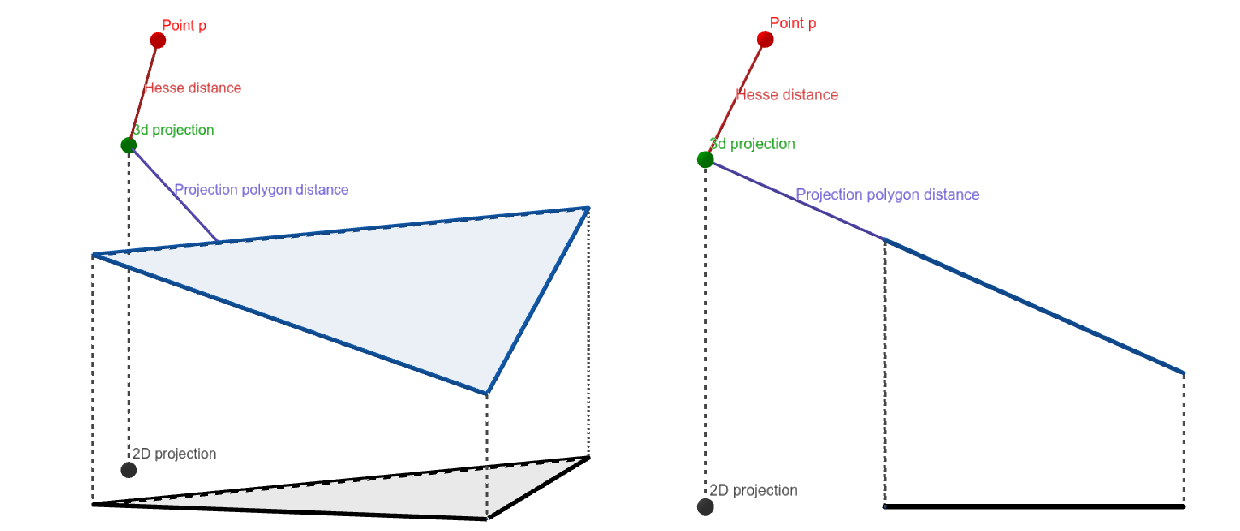
\includegraphics[width=\textwidth]{images/project}
	\caption{Illustration of the Hesse- and polygon projection distance. The point p (red) gets projected onto the infinitely extending global plane. Both the point projection (green) and the global planes convex hull (blue) get projected into 2D space (grey). The Hesse distance, i.e. the shortest distance to the infinitely extending plane (red), is shown as well as the minimum distance from the 2D point projection to the polygon (purple).}
	\label{fig:proj}
\end{figure*}

The Hesse-normal form describes the distance from the $i$-th transformed point $T(\vec{p}_i)$ to infinitely extending, $k$-th plane in 3D vector space
\begin{equation}\label{eq:hesse}
	D_{h}^{i,k} = \vec{n}_{\mathcal{P}_k} \cdot \left[ T(\vec{p}_i) - \vec{a}_{\mathcal{P}_k} \right] ,
\end{equation}
with normal $\vec{n}_{\mathcal{P}_k}$ and supporting point $\vec{a}_{\mathcal{P}_k}$ of the $k$-th plane.
The distance $D_{h}^{i,k}$ of the $i$-th point to the $k$-th plane reflects the length of the line segment, constructed from the $i$-th point to its projection on the $k$-th plane.
Therefore, by definition the line segment is parallel to the normal vector of the plane.
Thus, the $i$-th points projection $\widetilde{T}(\vec{p}_i)$ onto the $k$-th plane, which is required later, is easily calculated by shifting the point against normal direction:
\begin{equation}\label{eq:projection}
	\widetilde{T}(\vec{p}_i) = T(\vec{p}_i) - D_{h}^{i,k} \vec{n}_{\mathcal{P}_k}
\end{equation}

The simplicity of the Hesse distance is at contrast with its inability to take the extent of the plane into account.
Therefore, a second distance model is introduced: the polygon projection distance (PPD).
The convex hull represents the extend of a plane by forming a polygon with the outer most points that are assigned to a given plane. 
It is able to represent the expansion of the plane in all directions, and thus is utilized as a distance model.
To find the PPD, first a corresponding point gets projected onto the infinitely extending plane representation given by the Hesse form, i.e. $\widetilde{T}(\vec{p}_k)$ is found from eq.~\eqref{eq:projection} (green point in~\ref{fig:proj}).
Then, the 3D polygon, i.e. the points that make up the convex hull, as well as the corresponding 3D point projection, are projected again into a 2D vector space, using the maximal component of the normal vector of the plane.
E.g. in figure~\ref{fig:proj}, the blue planes normal vector has its mayor component in z-direction (upwards), thus the projection polygon distance is calculated in the xy-plane.
Using the maximum of the absolute magnitude of the normal vector ensures that the most sensible 2D projection is used for every direction.
Sunday et al.~\cite{pga} presents an optimal algorithm to check whether the point projection lies inside the polygon in 2D. 
If the point is inside the polygon, its PPD is set to zero.
If, however, the point is outside the polygon, the shortest distance to the polygon is calculated by looking at the minimum distance of the $i$-th point to each line segment, making up the convex hull of the $k$-th plane in 3D.
Let the polygon $P_k$ be made up of line segments $s_{m, j}$.
The line segment $s_{m, j}$ consists of the points $p_m$ and $p_j$.
The line segment is parameterized by
\begin{equation}
\label{eq:line}
	s_{m, j}(t) = p_m + t \cdot \left( p_j - p_m \right) ,  
\end{equation}
where $t \in \left[ 0, 1 \right]$. 
We set up a distance function, which measures the distance from the query point $p_i$ to an arbitrary point on the line segment.
\begin{equation}
	\label{eq:dist}
	d_{m, j}(t) = \lVert s_{m, j}(t) - p_i \rVert 
\end{equation} 
It is now possible to find the shortest distance to the line segment by finding the argument of the function that minimizes this distance.
Therefore, we set
\begin{equation}
	\pardiff{t} d_{m, j}(t)^2 \overset{!}{=} 0 ,
\end{equation}  
resulting in 
\begin{equation}
	t_0 = \frac{\left( p_j - p_m \right) \cdot \left( p_i - p_m \right)}{\left( p_j - p_m \right)^2} .
\end{equation}
Note the possibility of $t_0 \notin \left[ 0, 1 \right]$. 
In that case, the projection of the point $p_i$ onto the line given by eq.~\ref{eq:line} is not between $p_j$ and $p_m$. 
Instead, its projection onto the line falls outside of the segment.
By constraining $t_0$ we get 
\begin{equation}
\label{eq:minmax}
	\hat t = \min \left( \max \left( t_0, 0\right) , 1 \right) ,
\end{equation}
which is the argument that gives the shortest distance to the line segment, when inserted to eq. \ref{eq:dist}.
We find the PPD from the point $p_i$ to the polygon $P_k$ by calculating the minimum shortest distance over all line segments that make up the polygon.  

\subsubsection{Local Planar Clustering}

The presented algorithm employs LPC on each individual line scan.
The idea is to find planar features utilizing an optimized approximate k nearest neighbour (AKNN) search for normal calculation as in~\cite{aknnbbs}.
Thus, normals are calculated for every point in the respective line scan.
Then, the local normal model is combined with a region growing approach.
The region growing is implemented by storing the k-nearest neighbors in a queue, which represents the iteration order of the clustering algorithm.
A region grows if one of these neighbors has a distance shorter then a treshold $d_{growth}$ and additionally has a similar normal.
The angle between two normalized vectors is
\begin{equation}
\label{eq:smallestalpha}
	\alpha(\vec{n}_1, \vec{n}_2) = \arccos(\vec{n}_1 \cdot \vec{n}_2) \; .
\end{equation}
However, the \textit{smallest} angle between two \textit{normal} vectors is 
\begin{equation}
\label{eq:alphahat}
\hat \alpha(\vec{n}_1, \vec{n}_2) = 
\begin{cases}
	2\pi - \alpha(\vec{n}_1, \vec{n}_2) & \text{if  } \alpha(\vec{n}_1, \vec{n}_2) > \frac{3}{2} \pi \\
	\alpha(\vec{n}_1, \vec{n}_2) - \pi & \text{if  } \alpha(\vec{n}_1, \vec{n}_2) > \pi \\
	\pi - \alpha(\vec{n}_1, \vec{n}_2) & \text{if  } \alpha(\vec{n}_1, \vec{n}_2) > \frac{\pi}{2} 
\end{cases}
\; ,
\end{equation}
because the opposing normals $-\vec{n}_1$ and $-\vec{n}_2$ always have to be considered, since they correspond to the same plane.
We say that two normals are similar if the angle $\hat \alpha$ from eq. \ref{eq:alphahat} is smaller than a threshold $\epsilon_{\alpha}$. 

Planar areas like walls are therefore connected in one large cluster, while non-feature parts, i.e. non-planar or detached parts of the scan will have their own, smaller cluster.
You are then left with a rather easy task: filtering the clusters.
The filtering has two parts.
First, to combine clusters that are similar, i.e. have a short distance ($d_{growth}$) to each other and similar mean normals.
Second, to filter out all clusters that contain non-feature points.
Since all the non-feature points belong to small clusters, the presented algorihtm does this by putting a minimum threshold $N_{c,min}$ on the cluster size.
Figure \ref{fig:clustering} shows this concept on a real world dataset.
It was obtained by a floating sphere on a desk in an office environment, as described later in section \ref{sec:experimentalSetup}.

\begin{figure*}
	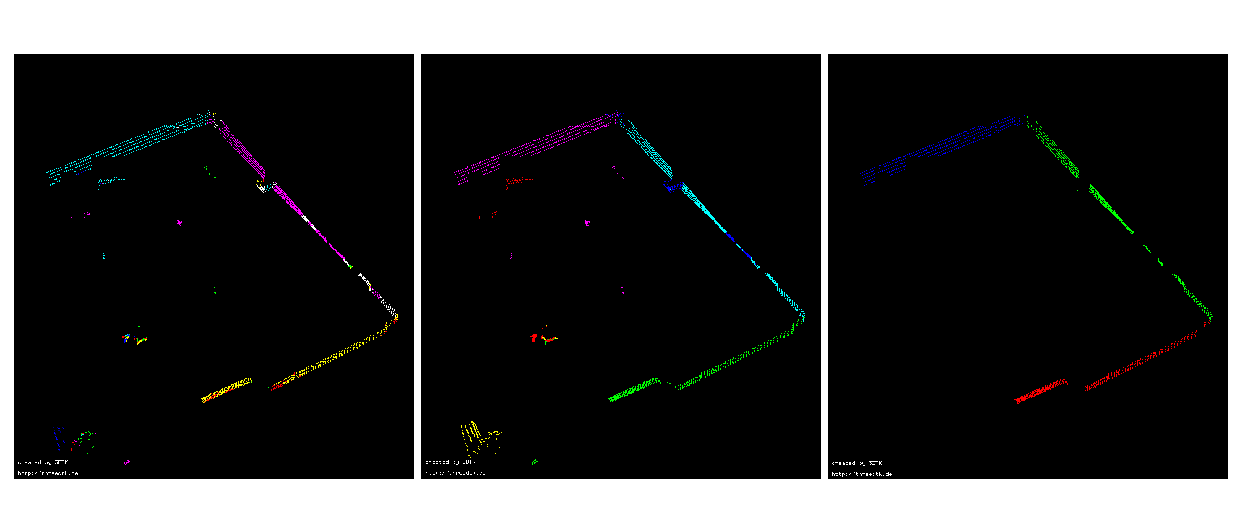
\includegraphics[width=\linewidth]{images/clustering}
	\caption{(Left) Point normals using the AKNN method with $K = 20$. (Middle) Result of the region growing, before applying the second filter. (Right) Resulting clusters after applying the second filter, using $N_{c,min} = 300$. }
	\label{fig:clustering}
\end{figure*}

Point-to-Plane correspondences are now established.
The distance models (Hesse + PPD) are utilized to check wether a cluster overlaps with any of the global planes, i.e. any point in the cluster has a Hesse distance smaller than some threshold $\epsilon_H$ and a PPD smaller than some additional threshold $\epsilon_P$, to the global plane.
For each overlap, we find the smallest angle between the corresponding cluster normal and the global plane normal, according to eq. \ref{eq:alphahat}.
Finally, a correspondence is established between all points in the cluster and the global plane, if the minimum angle between their normals is smaller than $\epsilon_\alpha$. 

\subsection{Optimization}

Assuming we now know the Hesse-normal form of all planes and all assigned points to these planes, we register the points to have a minimal distance to their respective planes.
The transformation $T(\vec{p}_i)$ of each point $\vec{p}_i$ with respect to a 6 DoF motion is described in homogeneous coordinates using the roll-pitch-yaw ($\varphi-\vartheta-\psi$) Tait-Brian angles as in~\cite{diebel2006representing}. Transforming the result back from homogeneous coordinates and using $C_a$ and $S_a$ to denote the cosine and sine of the angle in the subscript, and $t_a$ denoting the translation along the axis in the subscript yields:
\begin{align}
	T(\vec{p}_i)  =
    \resizebox{0.35\textwidth}{!}{$\begin{bmatrix}
        x_i C_\vartheta C_\psi - y_iC_\vartheta S_\psi + z_i S_\vartheta + t_x\\
        x_i (C_\varphi S_\psi + C_\psi S_\varphi S_\vartheta) + y_i(C_\varphi C_\psi - S_\varphi S_\vartheta S_\psi) - z_i C_\vartheta S_\varphi + t_y\\
        x_i(S_\varphi S_\psi - C_\varphi C_\psi S_\vartheta) + y_i(C_\psi S_\varphi + C_\varphi S_\vartheta S_\psi) + z_i C_\varphi C_\vartheta + t_z
    \end{bmatrix}$}
\end{align}
From this we define the function $D(\varphi,\vartheta,\psi,t_x,t_y,t_z, \vec{p}_i)$ that computes the distance of a point $\vec{p}_i$ to its corresponding plane $\mathcal{P}_k$.
Omitting the arguments of the function for simplicity:
\begin{align}
\begin{aligned}
    D &= T(\vec{p}_i) \cdot \vec{n}_{\mathcal{P}_k} \\
      &= n_{\mathcal{P}_k}^x (x_i C_\vartheta C_\psi - y_iC_\vartheta S_\psi + z_i S_\vartheta + t_x)\\
       &+ n_{\mathcal{P}_k}^y(x_i (C_\varphi S_\psi + C_\psi S_\varphi S_\vartheta)\\
       &\qquad+ y_i(C_\varphi C_\psi - S_\varphi S_\vartheta S_\psi) - z_i C_\vartheta S_\varphi + t_y)\\
       &+ n_{\mathcal{P}_k}^z (x_i(S_\varphi S_\psi - C_\varphi C_\psi S_\vartheta)\\
       &\qquad+ y_i(C_\psi S_\varphi + C_\varphi S_\vartheta S_\psi) + z_i C_\varphi C_\vartheta + t_z)\\
       &- \rho_{\mathcal{P}_k}
\end{aligned}
\end{align}

This distance function is what we want to minimize for all points and their respective planes.
Hence the error function $E$ is chosen as the square of the L2-norm of the distance:
\begin{align}
	E = \sum_{\forall \mathcal{P}_k}\sum_{\vec{p}_i \in \mathcal{P}_k} \norm[2]{D(\varphi,\vartheta,\psi,t_x,t_y,t_z, \vec{p}_i)}^2
\end{align}
Its gradient follows then immediately:
\begin{align}
	&\nabla E =  \sum_{\forall \mathcal{P}_k}\sum_{\vec{p}_i \in \mathcal{P}_k} \resizebox{0.28\textwidth}{!}{$\begin{bmatrix}\pardiff{\varphi} E&\pardiff{\vartheta} E&\pardiff{\psi} E&\pardiff{t_x} E&\pardiff{t_y} E&\pardiff{t_z} E\end{bmatrix}^T$}\\
    &\Rightarrow\nabla E = \resizebox{0.35\textwidth}{!}{$\sum_{\forall \mathcal{P}_k} \sum_{\vec{p}_i\in \mathcal{P}_k}2D(\vec{\Pi}, \vec{p}_i)\begin{bmatrix}\nabla E_\varphi &\nabla E_\vartheta & \nabla E_\psi & n_{\mathcal{P}_k}^x&n_{\mathcal{P}_k}^y&n_{\mathcal{P}_k}^z\end{bmatrix}^T$}
\end{align}
Where
\begin{align}
    &\begin{alignedat}{3}
        \nabla E_\varphi = &n_{\mathcal{P}_k}^y&&(x_i[-S_\varphi S_\psi+C_\varphi C_\psi S_\vartheta] \\&&&+y_i[-S_\varphi C_\psi -C_\varphi S_\vartheta S\psi] \\&&&- z_i C_\varphi C_\vartheta)\\
        &+ n_{\mathcal{P}_k}^z&&(x_i[C_\varphi S_\psi+C_\varphi C_\psi S_\vartheta] \\&&&+y_i[C_\varphi C_\psi -S_\varphi S_\vartheta S\psi] \\&&&- z_i S_\varphi C_\vartheta)
    \end{alignedat} \\
    &\begin{alignedat}{3}
        \nabla E_\vartheta = & n_{\mathcal{P}_k}^x(-x_iS_\vartheta C_\psi + y_i S_\vartheta S_\psi + z_iC_\vartheta) \\
        &+ n_{\mathcal{P}_k}^y(x_iC_\psi S_\varphi C_\vartheta - y_iS_\varphi C_\vartheta S_\psi + z_i S_\vartheta S_\varphi)  \\
        &+ n_{\mathcal{P}_i}^z(-x_iC_\varphi C_\psi C_\vartheta + y_iC_\varphi C_\vartheta S_\psi - z_i C_\varphi S_\vartheta)
    \end{alignedat}\\
    &\begin{alignedat}{3}
       \nabla E_\psi =& n_{\mathcal{P}_k}^x&&\left(-x_iC_\vartheta S_\psi - y_iC_\vartheta C_\psi\right) \\
       &+ n_{\mathcal{P}_k}^y&&(x_i[C_\varphi C_\psi - S_\varphi S_\vartheta S_\psi] \\
       &&&+ y_i[-C_\varphi S_\psi - S_\varphi S_\theta C_\psi]) \\
       &+ n_{\mathcal{P}_k}^z&&(x_i[S_\varphi C_\psi + C_\varphi S_\psi S_\theta] \\
       &&&+ y_i[-S_\psi S_ \varphi + C_\varphi S_\vartheta C_\psi]) 
    \end{alignedat}
\end{align}
and $\vec{\Pi}=\begin{bmatrix}\varphi & \vartheta & \psi & t_x & t_y & t_z\end{bmatrix}^T$.

As the gradient is well-defined we minimize the error function with any gradient based method. 
The commonly used, well-known stochastic gradient descent (SDG) algorithm computes 
\begin{align}
    \vec{\Pi}_{k+1} = \vec{\Pi}_{k} - \alpha \nabla E
\end{align}
where $\alpha$ is the learning rate.
To accelerate convergence and to improve the found solution further modifications are made.

Since we have vastly different effects on the error function by each dimension, the first consideration for improving the SDG is the following:
Typically, changes in orientation, i.e., the first three elements of the gradient vector $\pardiff{\varphi}E$, $\pardiff{\vartheta}E$, and $\pardiff{\psi}E$, have much more impact on the error function than a change in position.
This is intuitively explained since translating the scan makes the error grow linearly for all points.
However, when rotating the scan, points with a larger distance to the robot are moved drastically, leading to a higher sensibility on the error function.
For this reason, the $\alpha$ applied on orientation has to be much smaller than the $\alpha$ applied on the position.
It becomes obvious that $\alpha$ needs to be extended into vector form, $\boldsymbol\alpha$, therefore weighting each dimension differently.

Another consideration to speed up SDG is to adaptively recalculate $\boldsymbol\alpha$ for each iteration. 
We employ and modify ADADELTA as a technique to do so, which is described in detail in~\cite{zeiler2012adadelta}.
The main idea is the following:
It extends the SDG algorithm by two terms.
First, an exponentially decaying average of past gradients $\vec{G}_k$, which is recursively defined as
\begin{align}
    \vec{G}_{k+1} = \zeta \vec{G}_{k} + (1 - \zeta) {\nabla E}^2
\end{align}
and second, an exponentially decaying average of past changes $\vec{X}_k$, which is defined as
\begin{align}
    \vec{X}_{k+1} = \zeta \vec{X}_{k} + (1 - \zeta) {\boldsymbol\alpha \nabla E}^2
\end{align}
where $\zeta \leq 1$ is a decay constant, typically close to $1$.
The root mean squared (RMS) of these quantities are
\begin{align}
    RMS[\vec{G}]_{k} = \sqrt{\vec{G}_{k} + \epsilon_{num}}
\end{align}
and 
\begin{align}
    RMS[\vec{X}]_{k} = \sqrt{\vec{X}_{k} + \epsilon_{num}}
\end{align}
where $\epsilon_{num} > 0$ is a very small constant, typically close to $0$ (Note: this is a different threshold as the one used in section~\ref{sec:point-to-plane-correspondences}).
It will prevent dividing by zero in the recalculation of $\boldsymbol\alpha$, which is as follows:
\begin{align}
    \boldsymbol\alpha_{k} = \frac{RMS[X]_{k-1}}{RMS[G]_{k}}
    \label{eq:adadeltaalphaupdate}
\end{align} 
For our particular application, ADADELTA behaves a little too aggressively.
Despite giving a good measure on how to adapt $\boldsymbol\alpha$, the algorithm sometimes overshoots, and does not converge.
Therefore, we employ another scaling factor, typically not found in ADADELTA, extending eq.~\eqref{eq:adadeltaalphaupdate} to:
\begin{align}
    \boldsymbol\alpha_{k} = \boldsymbol\alpha_0 \cdot \frac{RMS[X]_{k-1}}{RMS[G]_{k}}
    \label{eq:adafinalized}
\end{align} 
where $\boldsymbol\alpha_0 $ holds the scaling factors for each dimension.

Finally, the SDG model is improved using eq.~\eqref{eq:adafinalized} and extends to 
\begin{align}
    \vec{\Pi}_{k+1} = \vec{\Pi}_{k} - \boldsymbol\alpha_0  \frac{RMS[X]_{k-1}}{RMS[G]_{k}} \cdot \nabla E
\end{align}
Using this algorithm once after finding correspondences from points to planes leads to convergence to a local minimum, which is often not an optimal solution.
Even if we increase the number of iterations dramatically, no better solution than the local minimum is found.
That is unless you consider updating the correspondence model after $i$ iterations of gradient descent.
Re-assigning point-to-plane correspondences this way $k$ times, with a large enough $k$, leads to an optimal solution after maximum $n = k\cdot i$ iterations of gradient descent.

\subsection{Further Optimizations of the Algorithm}

The algorithm was extended by two further optimizations, which are helpful in different scenarios.

Firstly, we introduce the possibility to choose a lock on some dimensions from being optimized by setting the corresponding $\alpha_i$ to zero.
Although 6D optimization generally works, reducing the optimization space is particularly useful if the source of error in the system is known and a model exists.
That way, e.g., as we expect a spherical robot to move on a plane the position along the axis perpendicular to the plane is constant and should not be used for optimization.\todo{@Fabi clarify in experiments which locks were active.} 

Secondly, we employ a continuous iteration, where the scans are processed sequentially. 
This is especially useful for mobile systems, where pose errors accumulate due to increasing tracking uncertainties.
The assumption is that the error in one scan is also present in the following scan, plus some unknown new error.
We eliminate the error from scan $m$ which is also present in scan $m+1$ by applying the pose change from scan $m$, $\vec{\Pi}_{n,m} - \vec{\Pi}_{0,m}$ after $n$ gradient descent iterations, to scan $m+1$, before restarting gradient descent.

To quantify the quality of the proposed registration method, it is tested on simulated as well as on real world data. 

%!TEX root = ../main.tex
\section{Simulation}

For the simulated data we implemented a noisy world-robot-sensor model.  
We are simulating a LIVOX-Mid100~\cite{LivoxMid40-100} laser scanner with customizable noise level on the range measurements inside a robot with different motion capabilities, subject to noise in its pose estimation. This yields scan results similar to the ones obtained in the real world.

\subsection{Range Noise Model}

Most real laser scanners are subjected to range measurement noise that is proportional to the measured range. 
Therefore the simulated sensors are as well. 
To achieve this we sample a noise percentage $n_P$ from some normal distribution $\mathcal{N}(\mu,\sigma^2)$. 
The resulting range $r$ given the true range $r_t$ is then
\begin{align}
	r = r_t(1+n_P)
\end{align}
For each measurement ray the noise percentage is sampled independently. 

\subsection{Pose Estimation Noise Model} 

For the pose measurement one cannot simply add white noise to the current pose estimate as this does not capture the integration error which is common among inertial measurement units (IMU). 
Therefore we assume a disturbance torque about the two axes that lie in the ground plane. 
This is equivalent to a case, where a slightly shifted ground plane or a unbalanced locomotion system of the robot is present.  

Accordingly, a spherical robot that is assumed to be translating exactly along one axis by rotation exactly about one other axis at an angular velocity $\omega$  experiences random disturbance torques at each time instant that accelerate the sphere's rotation about the respective axes. 
This additional motion is determined by integrating the disturbance torques which are sampled from some normal distribution $n_\phi, n_\psi \in \mathcal{N}(\mu,\sigma^2)$ each.  
The pose update in the discrete simulation is therefore given by: 
\begin{align}
	\begin{bmatrix}\varphi\\\vartheta\\\psi\\x\\y\\z\end{bmatrix}_{k+1} = 
	\begin{bmatrix}\varphi\\\vartheta\\\psi\\x\\y\\z\end{bmatrix}_{k} 
	+ \begin{bmatrix}1\\0\\0\\R\\0\\0\end{bmatrix}\omega \Delta t  + \Delta t \underbrace{\sum_{i = 0}^k \begin{bmatrix}n_\varphi[i] \Delta t\\0\\n_\psi[i]\Delta t\\0\\0\\0\end{bmatrix}}_{\substack{\text{Difference in}\\\text{angular velocity}}}
\end{align}

Assuming intended locomotion along the $z$-axis and unintended locomotion along the $x$-axis where $R$ is the sphere radius.
No movement upwards is possible since the robot moves on a flat ground, hence the entry is zero.

\subsection{Simulated Datasets}

Figure~\ref{fig:simulatedDatasets} shows a noise free trajectory through a simulated environment as well as a trajectory with noisy sensors.
In the noise-free case, the trajectory slightly bends in the direction of disturbance torque sideways while also varying in velocity in the intended direction of travel.
In the noisy case the ideal straight trajectory is assumed, hence the planes enclosing the room are sensed multiple times. 
In particular we see that the trajectory of the robot leads through one of the sensed planes. 
Also, the further the sensed points are the noisier they appear, which is consistent with the larger influence of the pose error at higher distances.  

\begin{figure*}
	\centering
	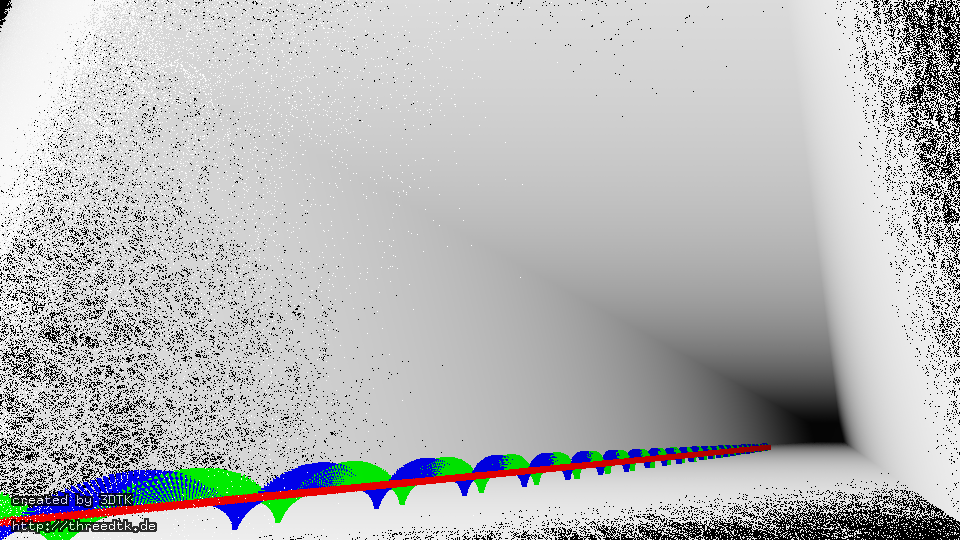
\includegraphics[width=0.51\textwidth]{images/perfect_bottom}\hfill
	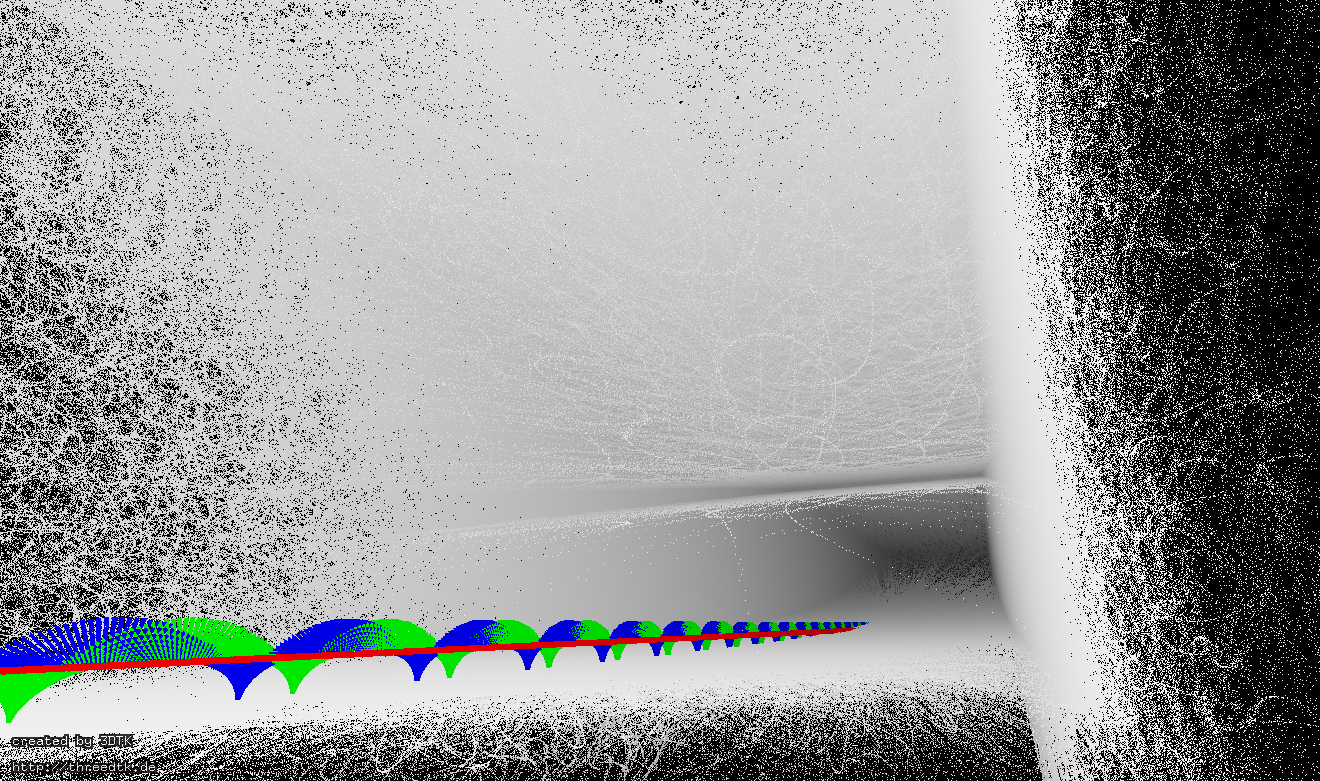
\includegraphics[width=0.48\textwidth]{images/noisy_pose_and_range_bottom}\\
	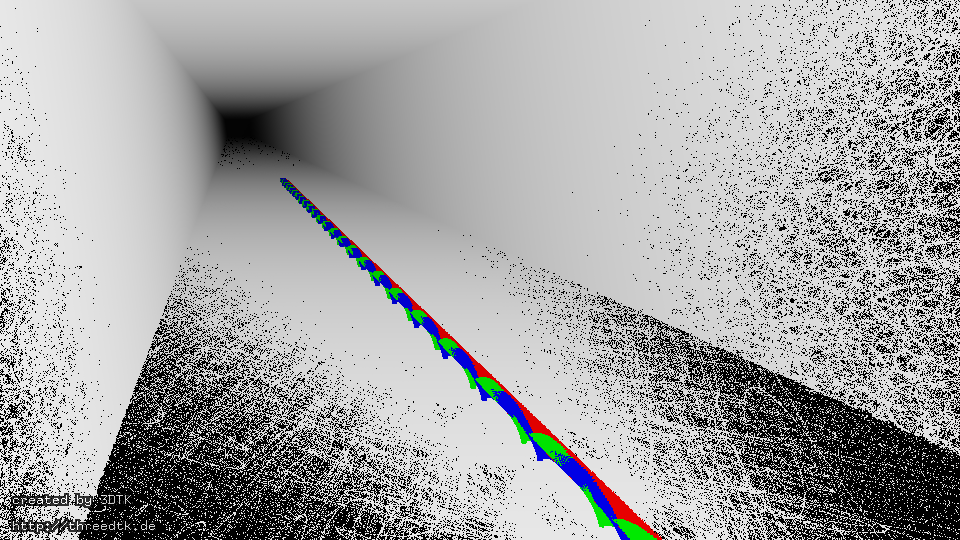
\includegraphics[width=0.51\textwidth]{images/perfect_top}\hfill
	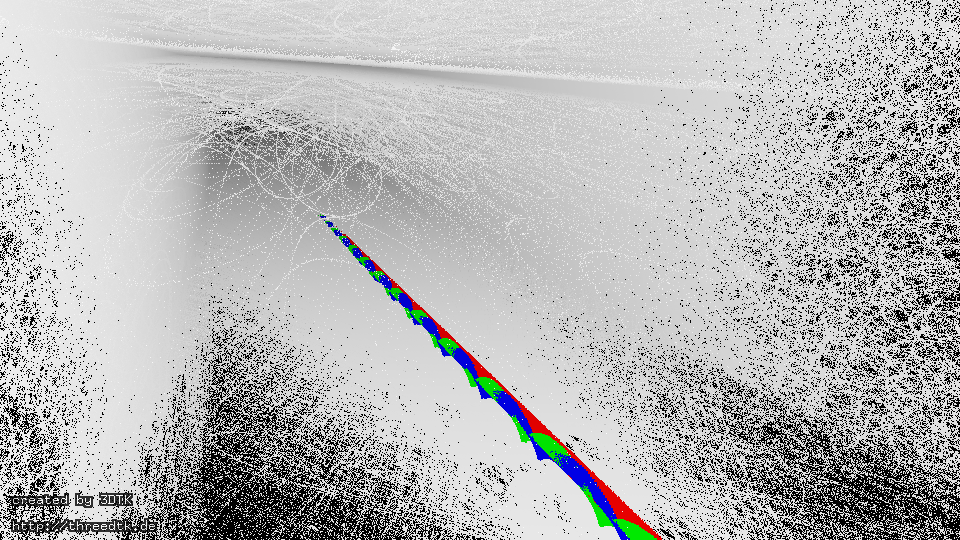
\includegraphics[width=0.48\textwidth]{images/noisy_pose_and_range_top}\\
	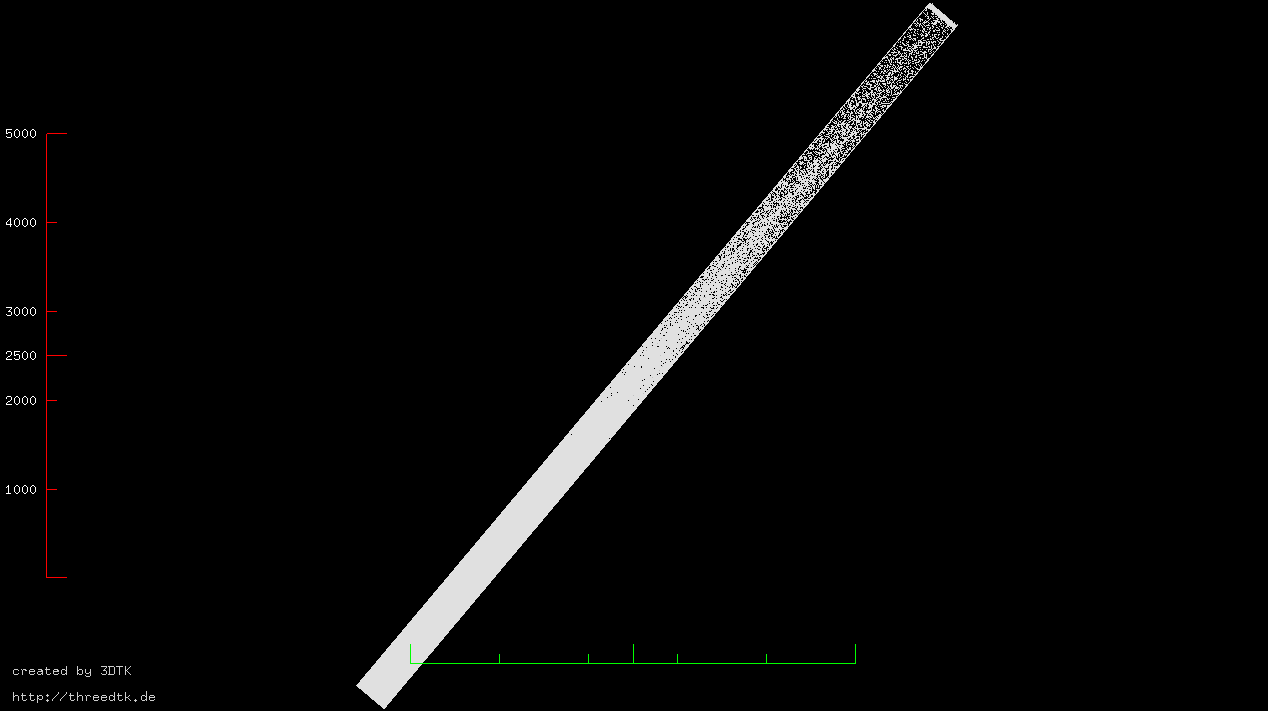
\includegraphics[width=0.51\textwidth]{images/perfect_top_view}\hfill
	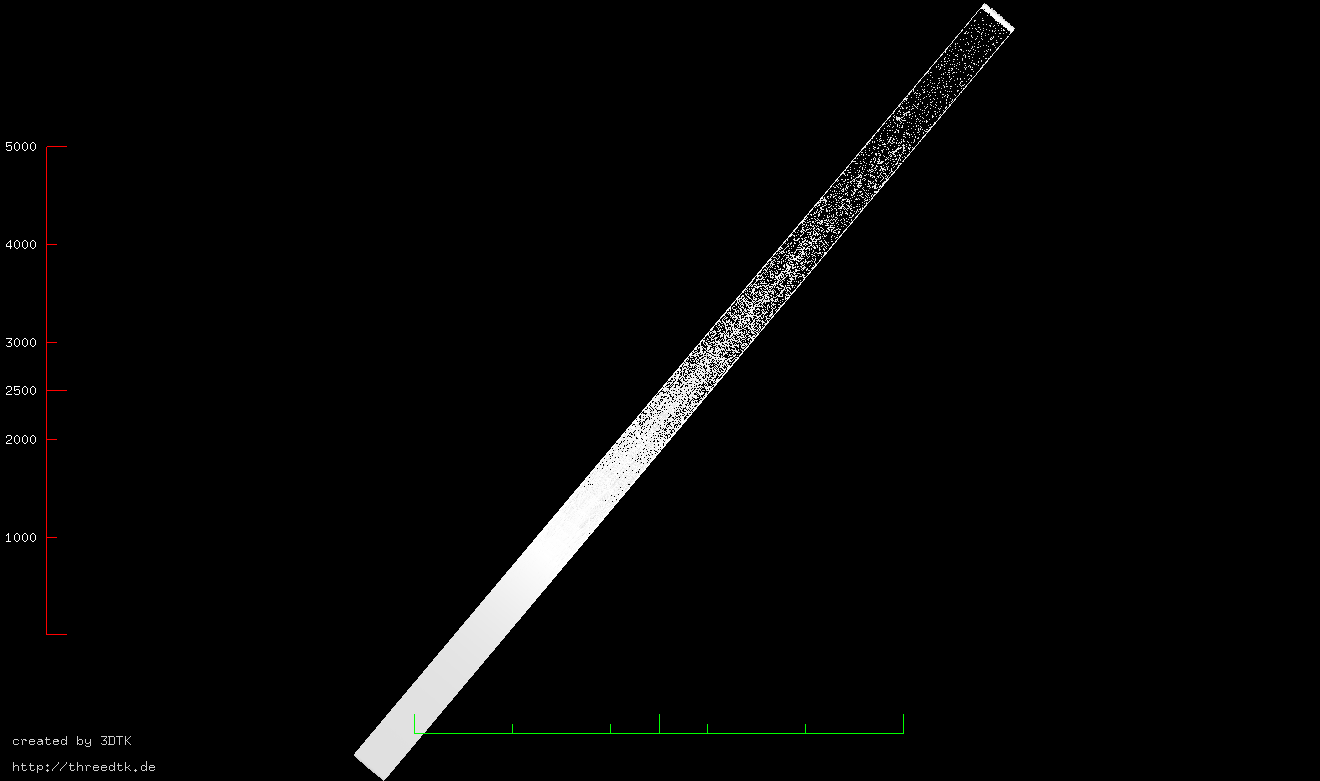
\includegraphics[width=0.48\textwidth]{images/noisy_pose_and_range_top_view}\\\vspace{0.5cm}
	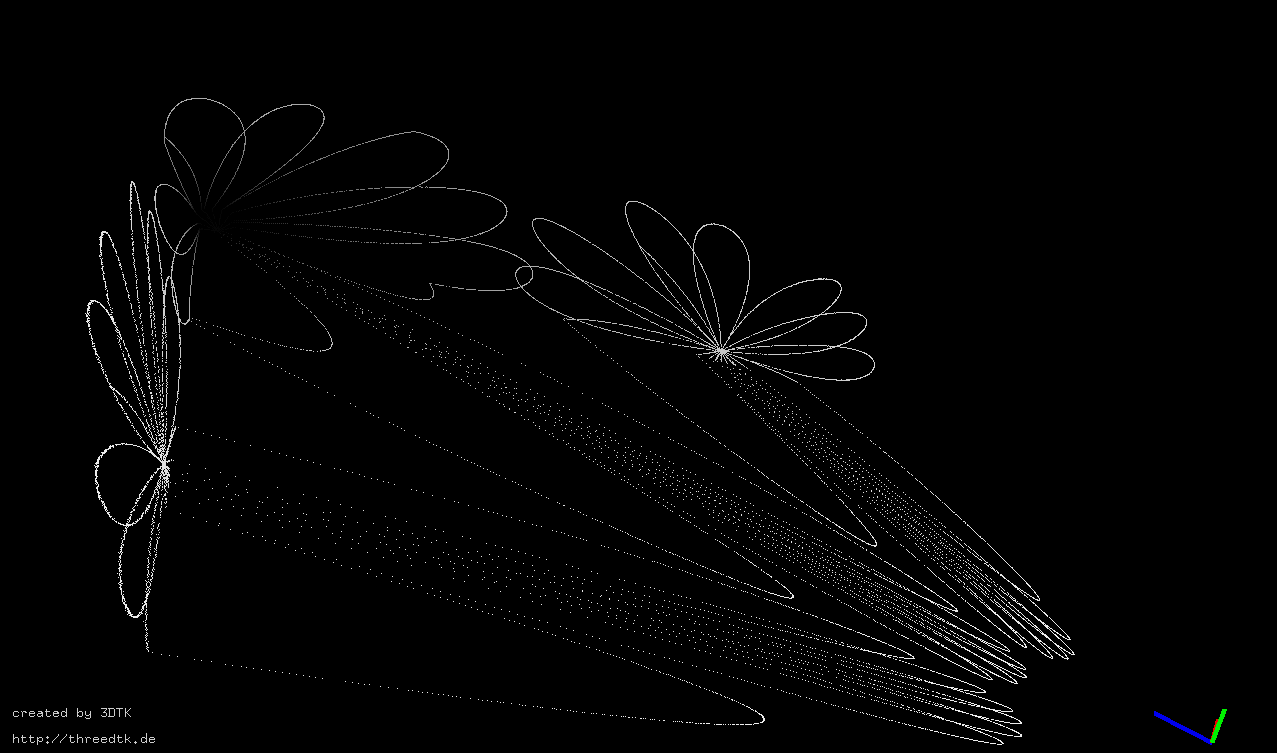
\includegraphics[width=0.25\textwidth]{images/sim_frame_00.png}\hfill
	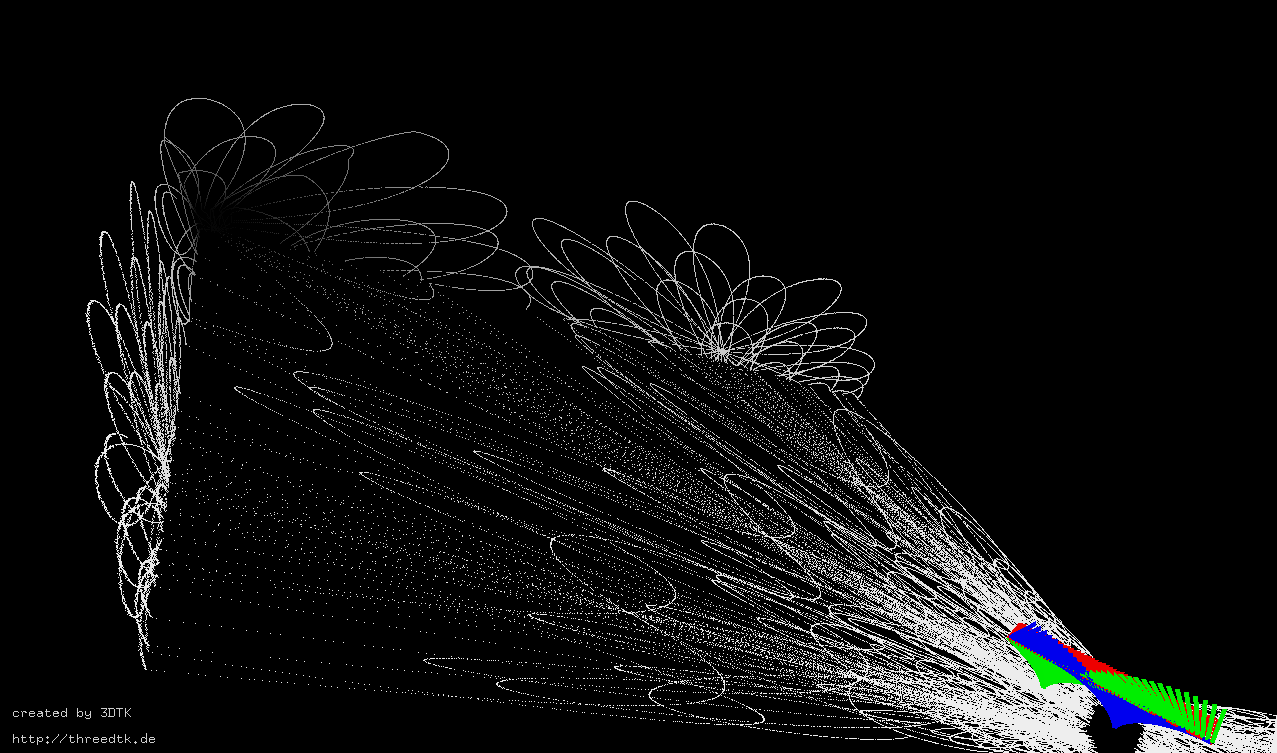
\includegraphics[width=0.25\textwidth]{images/sim_frame_02.png}\hfill
	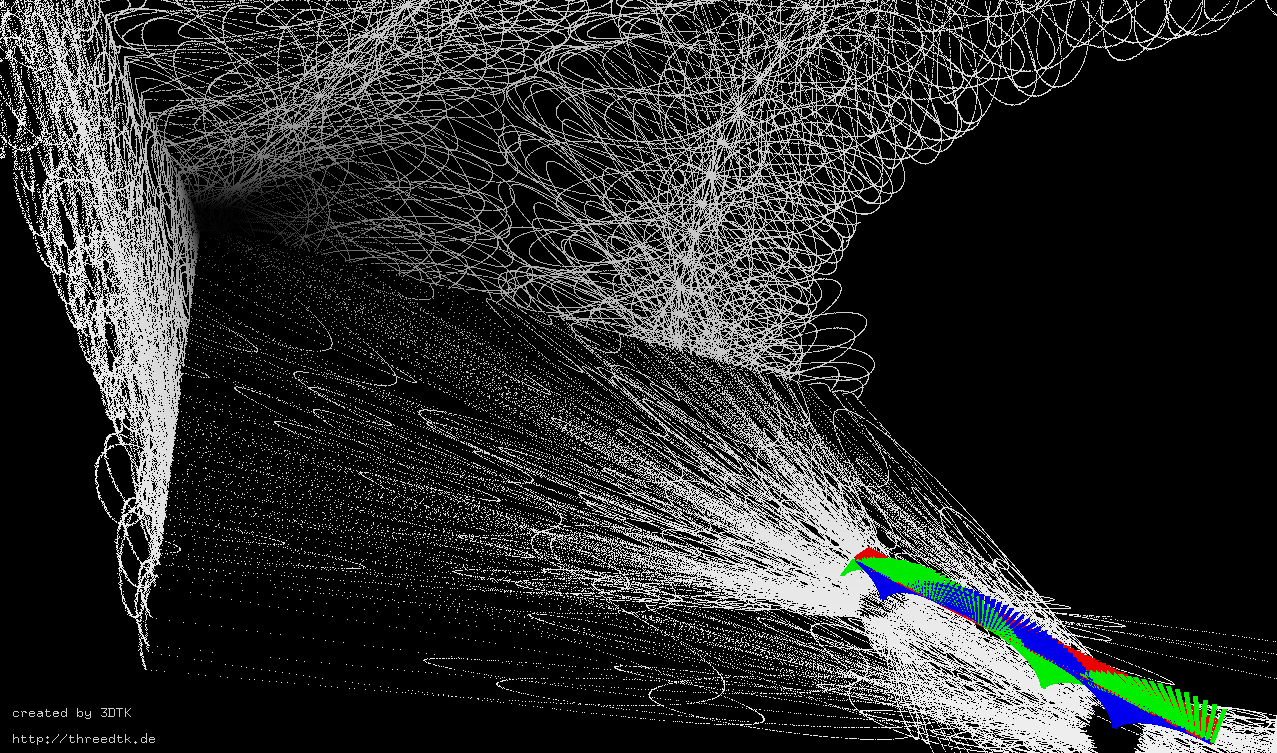
\includegraphics[width=0.25\textwidth]{images/sim_frame_06.png}\hfill
	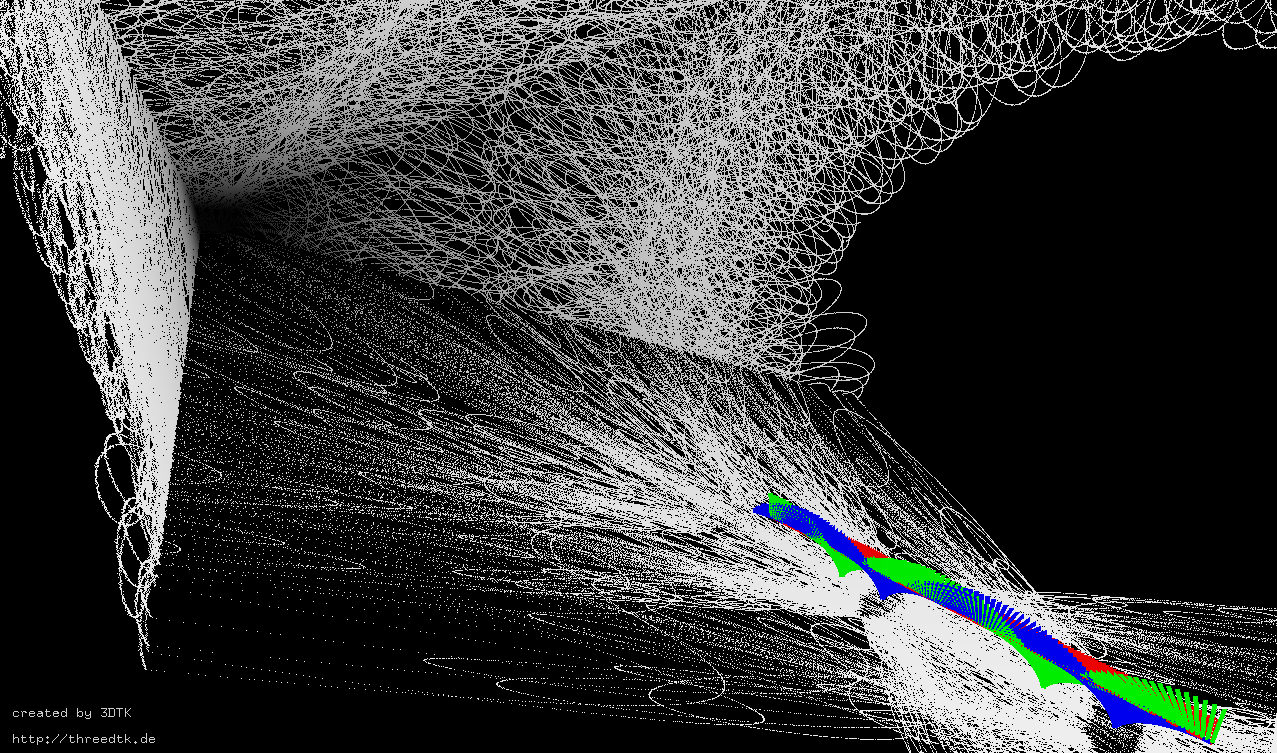
\includegraphics[width=0.25\textwidth]{images/sim_frame_08.png}
	\caption{Two simulated datasets of a long hallway of size $\SI{4}{\meter}\times\SI{3}{\meter}\times\SI{100}{\meter}$. Ideal noise free (left), noisy pose ($\mathcal{N}_\varphi = \mathcal{N}_\psi(\mu = 0.0001, \sigma= 0.00001)$) and noisy range measurements ($\mathcal{N}_r(\mu = 0, \sigma = 0.001)$) (right). Below: Initial sequence of the simulation of the ideal dataset showing the simulated motion of the robot.}
	\label{fig:simulatedDatasets}
\end{figure*}

%!TEX root = ../main.tex
\section{Experimental Setup}\label{sec:experimentalSetup}

We also tested out algorithm on a real-world dataset that adheres to different motion profiles and laser scanners type with different scanning patterns than the simulated data.  

The dataset is collected by a line scanner, in particular a SICK LMS141 industrial scanner, inside a sphere of a diameter of \SI{20}{\centi\meter} that lies on a floating desk, which is air-pressurized, such that the sphere is hovering.
On this floating desk, the sphere can rotate freely about all axis while being fixed in position. 
Hence, in this experiment the optimization space can be reduced to a rotation.
Further, without the motion, the 2D laser cannot obtain a 3D model from the environment, thus requiring registration. 
The sphere is equipped with a low-cost IMU, i.e., a PhidgetSpatial Precision 3/3/3, to estimate the orientation. 

Figure~\ref{fig:float-sat-sphere} shows the experimental setup. TThe left column of figure~\ref{fig:cylon-corrected} shows the pre-registered resulting point cloud . 
We see that the point cloud is rather noisy, and in particular, the walls are sensed multiple times, hence appearing very blurry. 

\begin{figure}
	\centering
	\begin{minipage}[c]{0.45\textwidth}
		\centering
		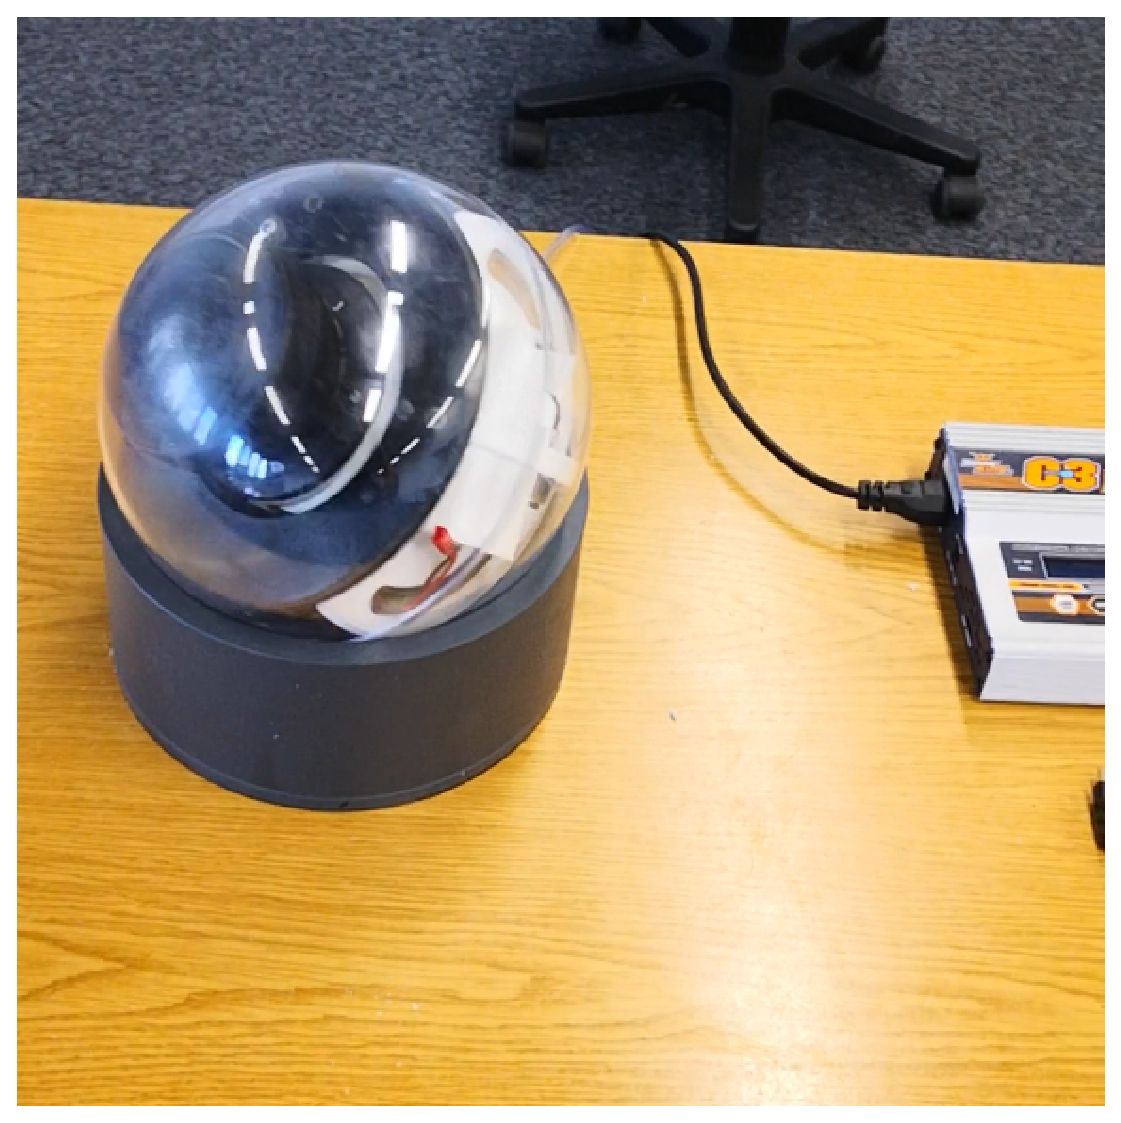
\includegraphics[width=0.33\textwidth, height=0.33\textwidth]{./images/sphere-frame-1.eps}\hfill
		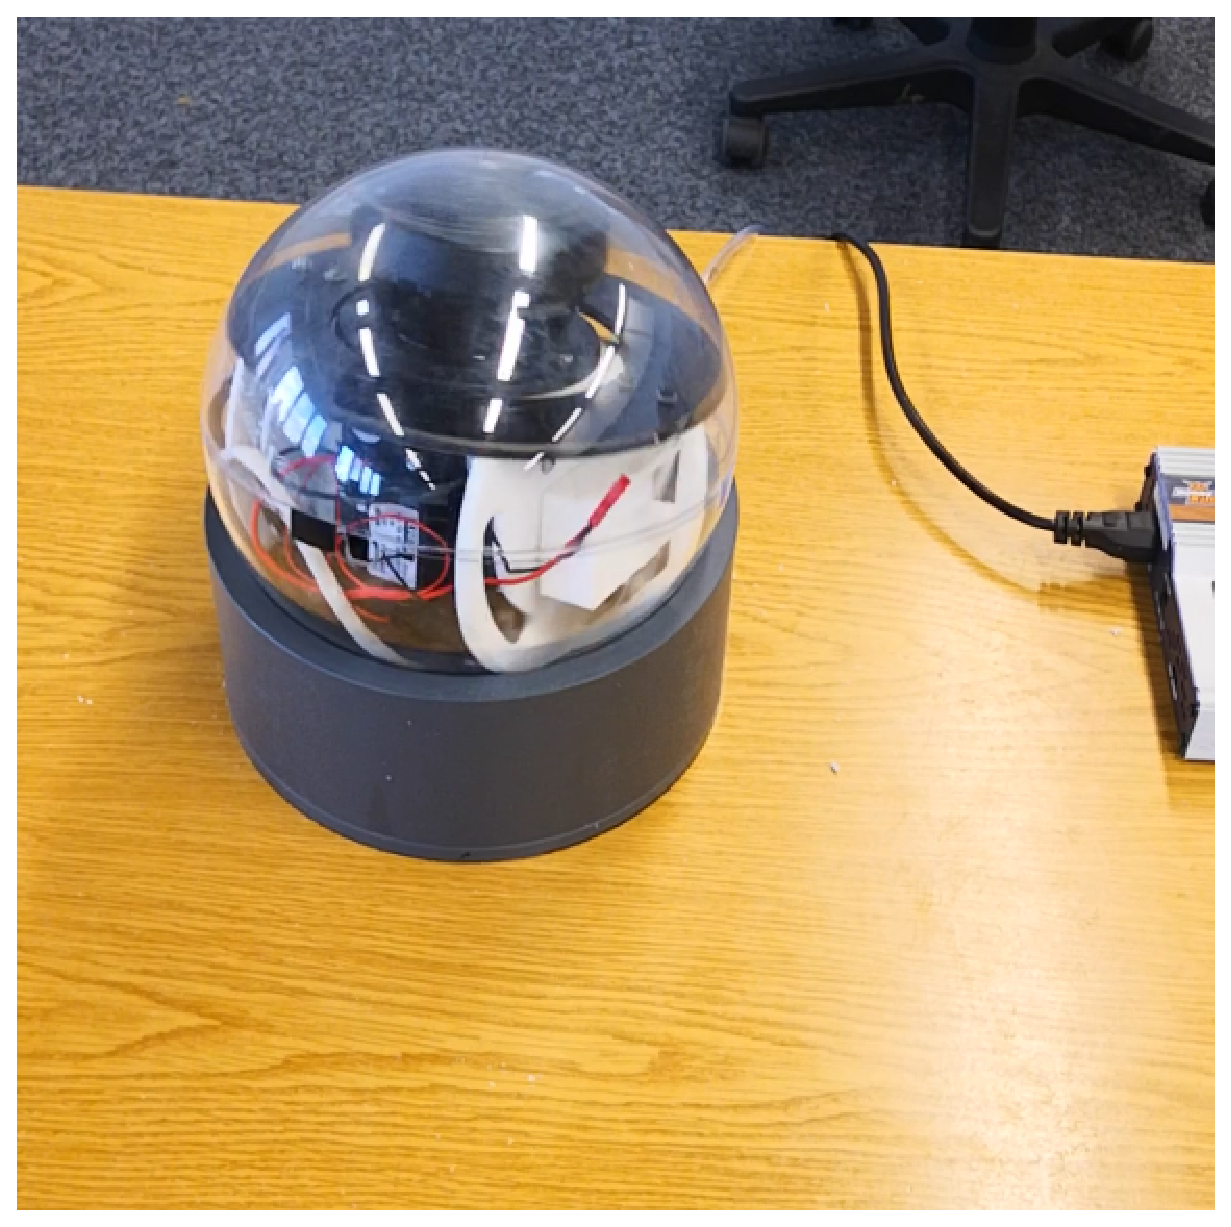
\includegraphics[width=0.33\textwidth, height=0.33\textwidth]{./images/sphere-frame-2.eps}\hfill
		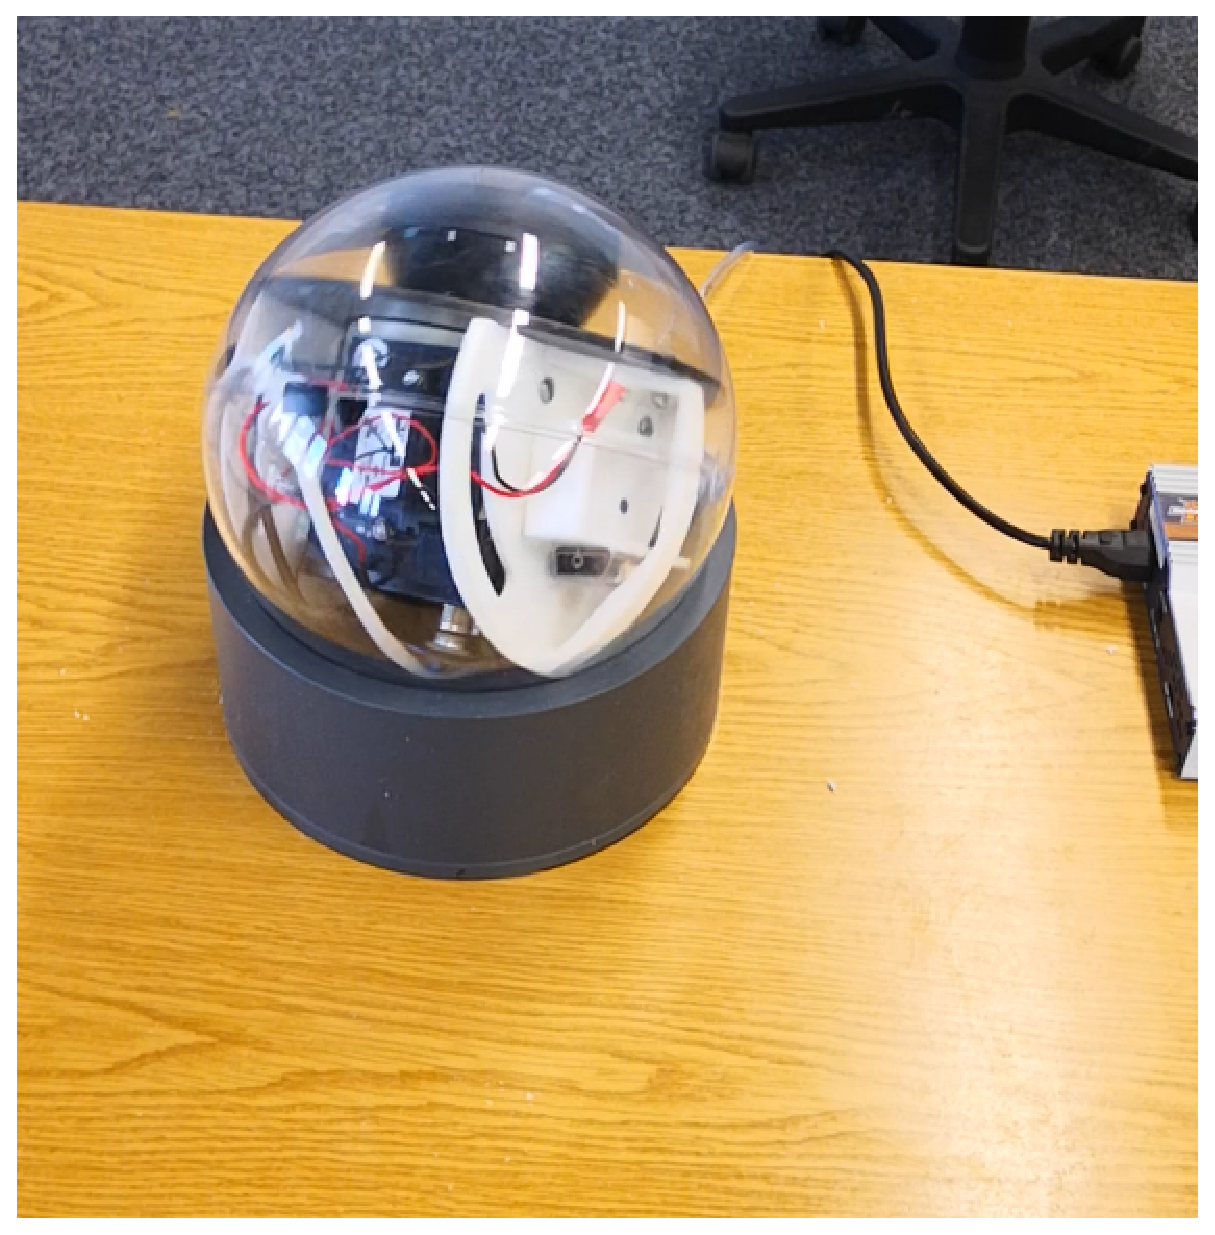
\includegraphics[width=0.33\textwidth, height=0.33\textwidth]{./images/sphere-frame-3.eps}\\
		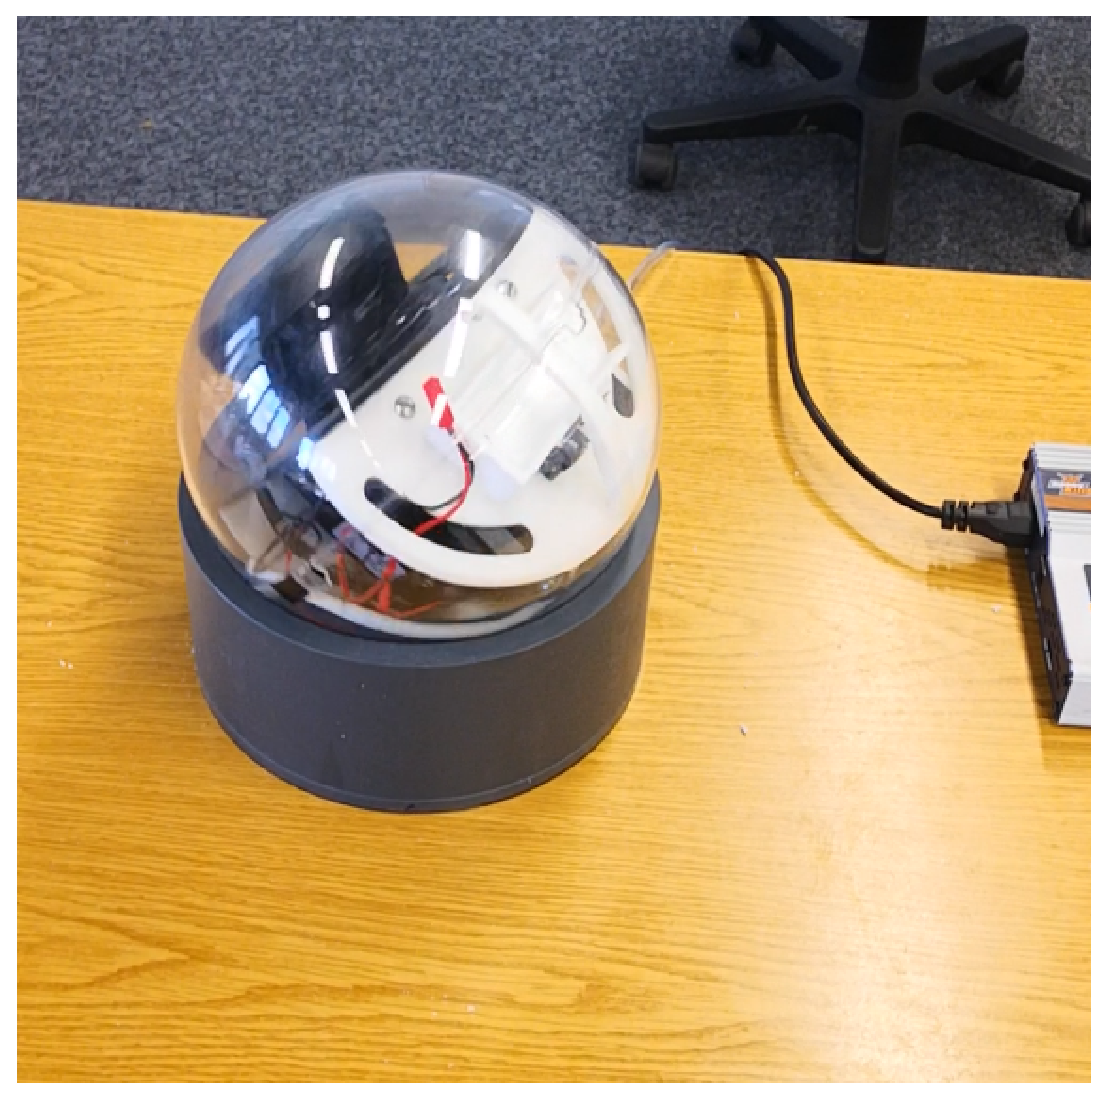
\includegraphics[width=0.33\textwidth, height=0.33\textwidth]{./images/sphere-frame-4.eps}\hfill
		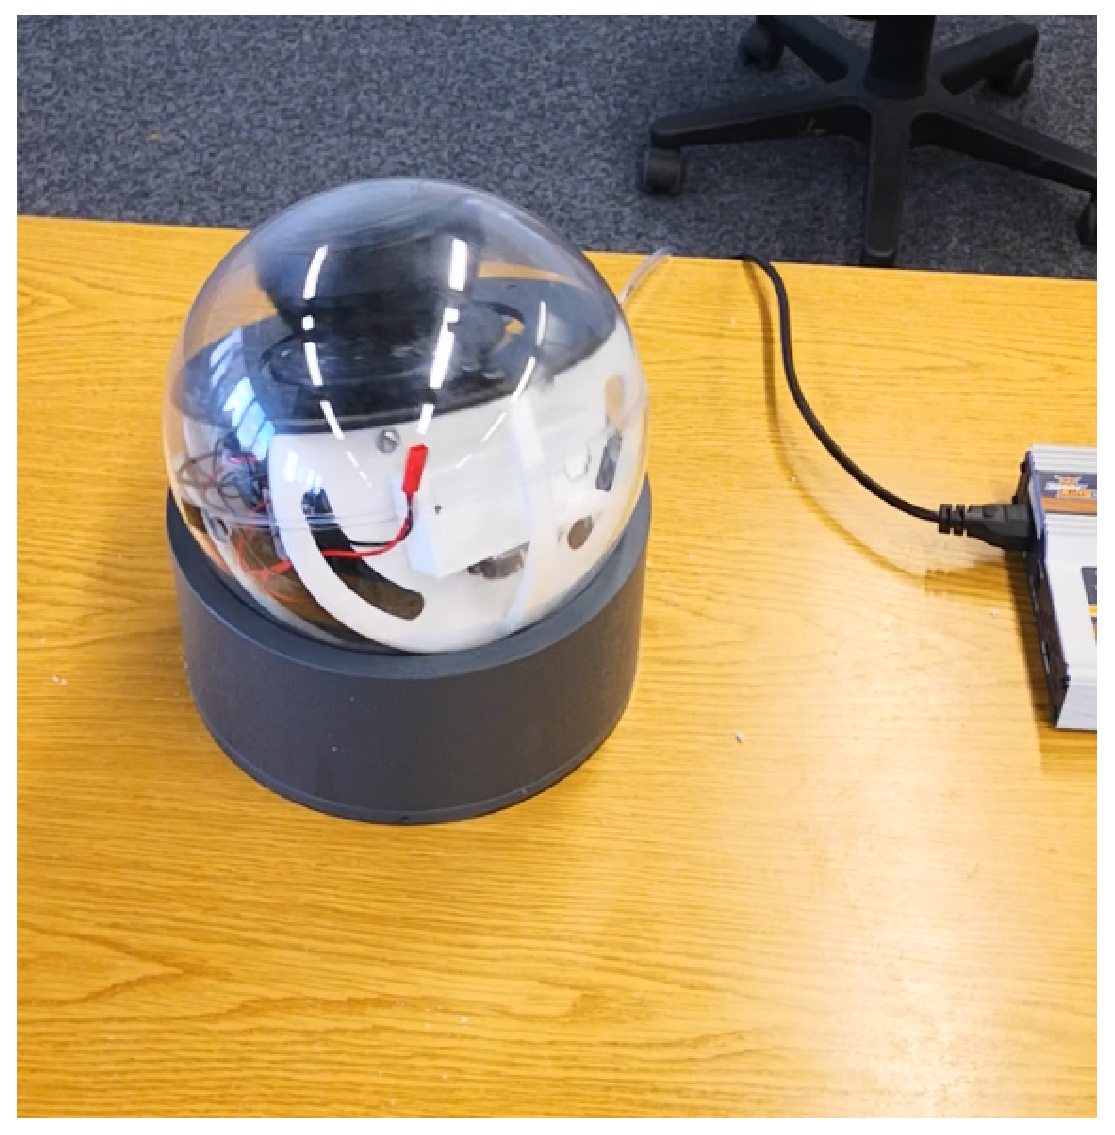
\includegraphics[width=0.33\textwidth, height=0.33\textwidth]{./images/sphere-frame-5.eps}\hfill
		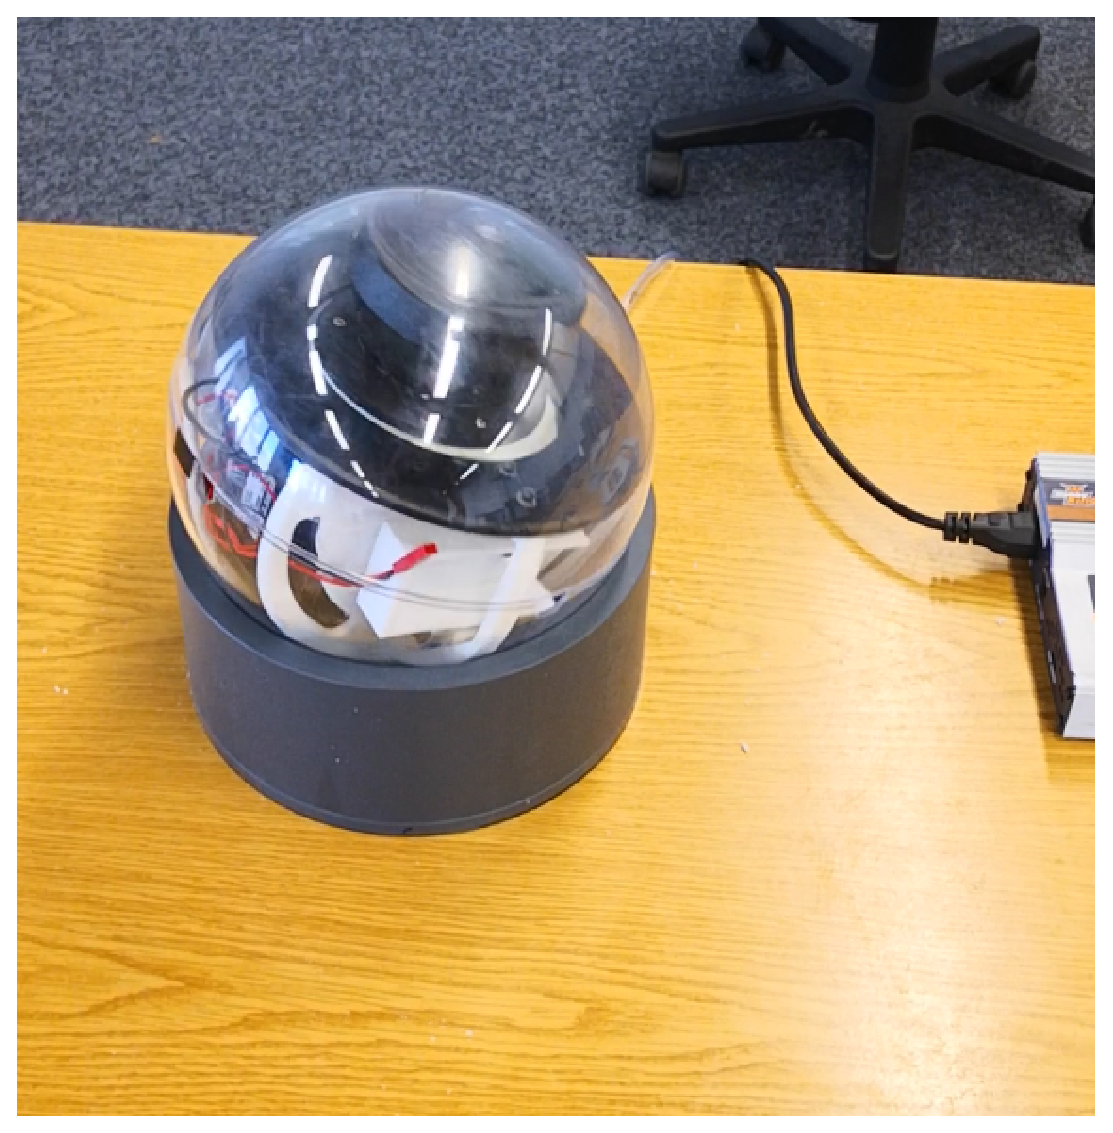
\includegraphics[width=0.33\textwidth, height=0.33\textwidth]{./images/sphere-frame-6.eps}\hfill
	\end{minipage}\\
	\vspace{0.1cm}
	\begin{minipage}[c]{0.45\textwidth}
		\centering
		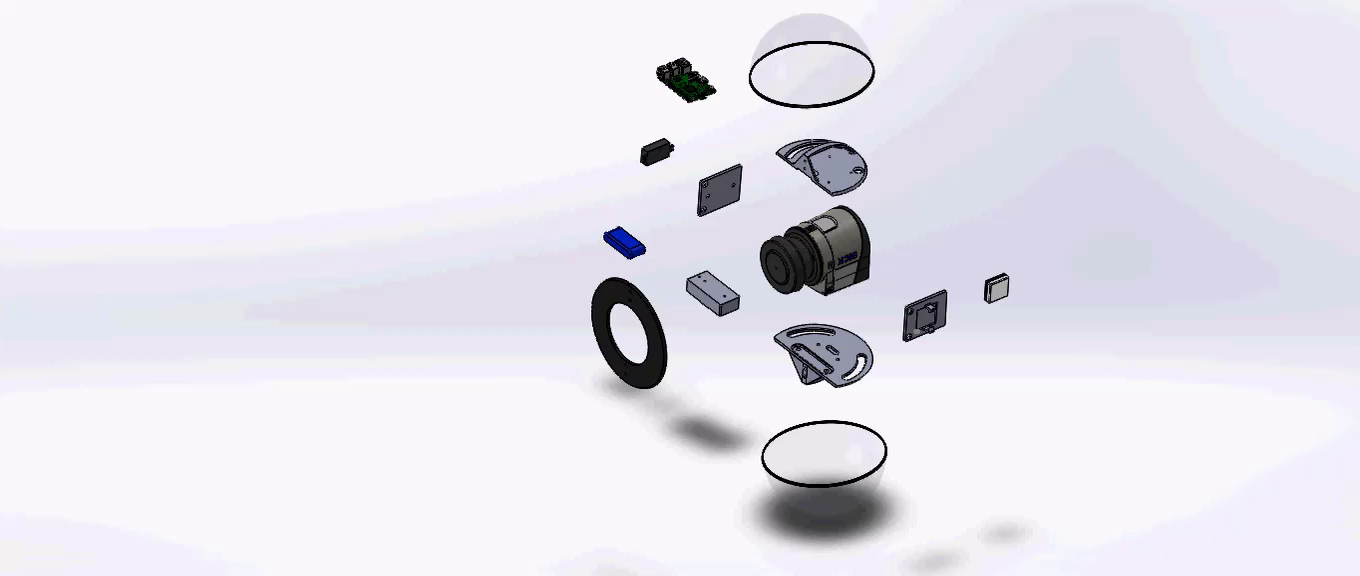
\includegraphics[width=0.49\textwidth, trim={20cm 0 10cm 0}, clip]{./images/cylon-exploded}\hfill
		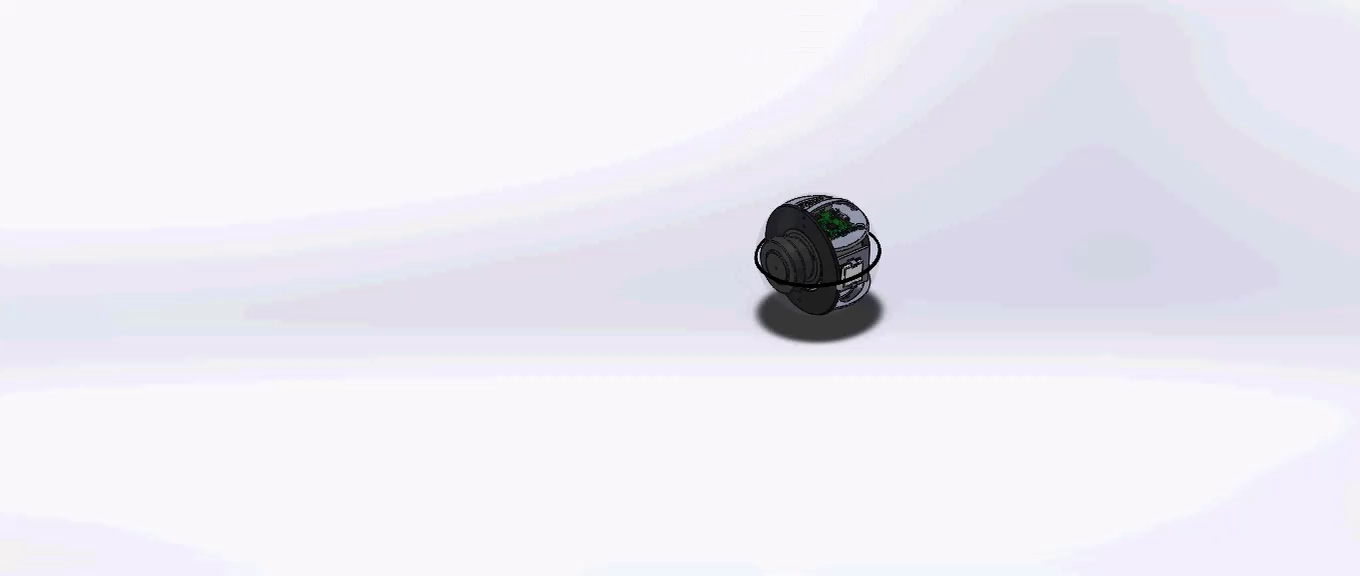
\includegraphics[width=0.49\textwidth, trim={20cm 0 10cm 0}, clip]{./images/cylon-setup}\hfill
	\end{minipage}
	\caption{Data acquisition using floating sphere. Top: A sequence of orientations the sphere assumes during data acquisition. Bottom: Hardware setup of the sphere.} 
	\label{fig:float-sat-sphere}
\end{figure}

\iffalse % This is commented out because we couldn't produce results
	\subsection{RADLER}

	The second dataset is recorded using the RADLER system as described in~\cite{Borrmann2020-RADLER}.
	While not a spherical robot, this system shows many similarities with respect to its motion with a spherical robot.
	The system was manually steered along with a squared set of hallways that loop back to the initial starting point inside the old mathematics building at the University of Würzburg (denoted ``The Circle'' in~\cite{Borrmann2020-RADLER}).

	Figure~\ref{fig:radler-mathe} shows the system setup as well as the resulting point cloud.
	We see that with continuing measurement time, the drift increases, and the hallways are senses multiple times with a clear offset to each other. 

	\begin{figure*}
		\centering
		\begin{minipage}[c]{\textwidth}
			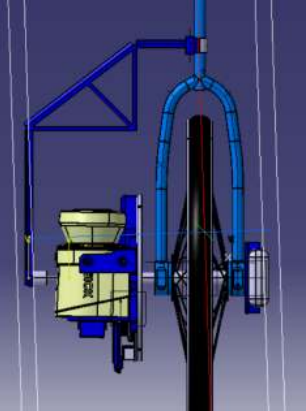
\includegraphics[width=0.2925\textwidth]{./images/radler_setup}\hfill
			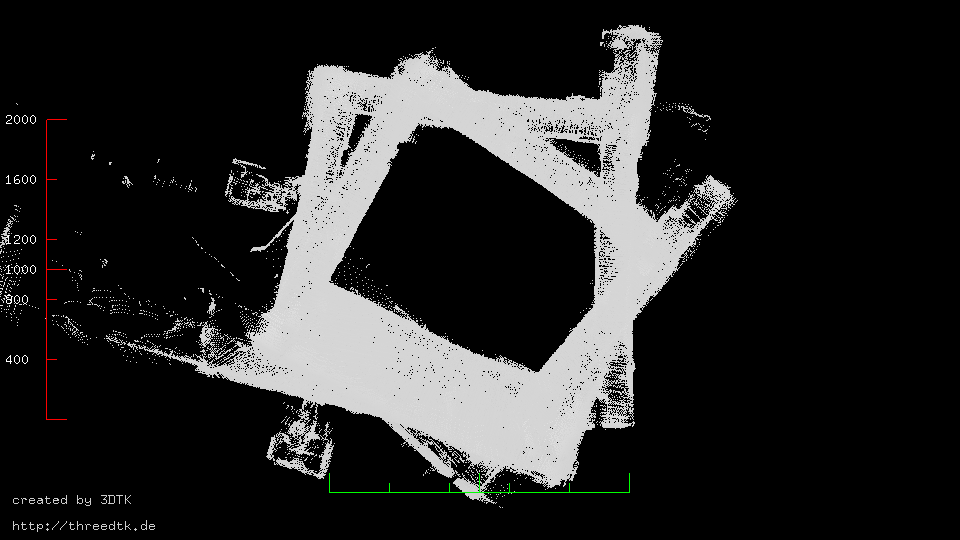
\includegraphics[width=0.7\textwidth]{./images/mathe_top_view}
		\end{minipage}
		\caption{Data acquisition using the RADLER system. Left: System setup (courtesy of Borrmann~\cite{Borrmann2020-RADLER}). Right: Unprocessed resulting point cloud.}
		\label{fig:radler-mathe}
	\end{figure*}

	\subsection{Descend Sphere REMOVE THIS SECTION}

	This was recorded using a LIVOX-Mid 100 laser scanner mounted inside a transparent shell. 
	The robot contained three Phidget 3/3/3 Spatial IMUs and was attached to a \SI{50}{\meter} tether cable that was rolled on a spool which in turn was connected to an angular encoder. 
	From these sensors, we obtained orientation information as well as height information. 
	The setup was then brought into a high indoor building (\href{https://www.sfs-w.de/feuerwehrschule/virtueller-rundgang.html}{Firefighter School in Würzburg}) where the system was manually descended from a balcony scanning the building interior.
	The robot covered a distance of approximately \SI{22}{\meter} in about \SI{402}{\second}.
	Additionally, the building was scanned using a terrestrial laser scanner to provide a reference.
	The measurements were then rigidly corrected before applying our plane-based correction. 
	Figure~\ref{fig:experimental-setup} shows the acquired 3D point clouds and the experimental setup. 

	\begin{figure}
		\centering
		\begin{minipage}[c]{0.25\textwidth}
			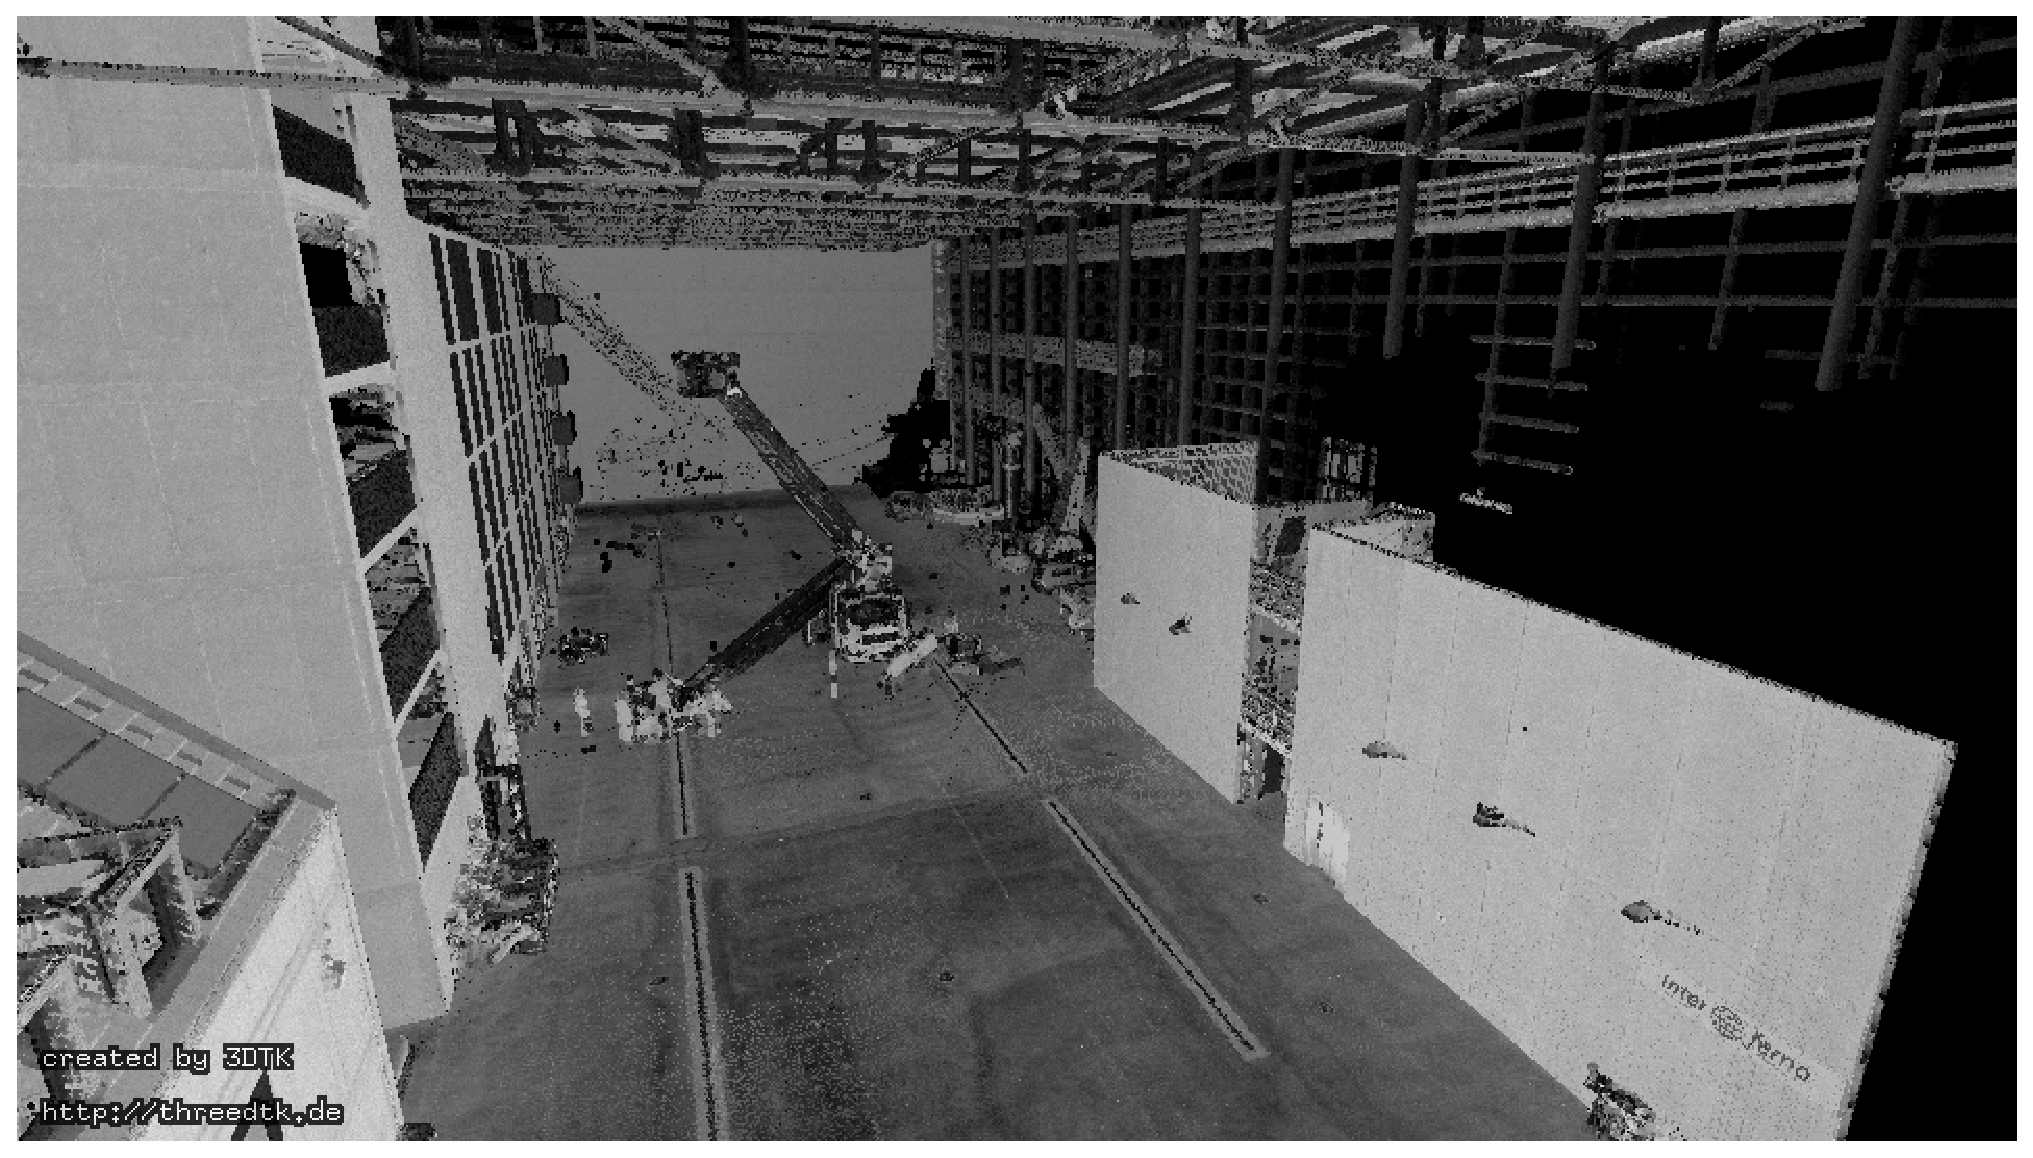
\includegraphics[width=\textwidth]{images/scan-riegl-fire}\\
			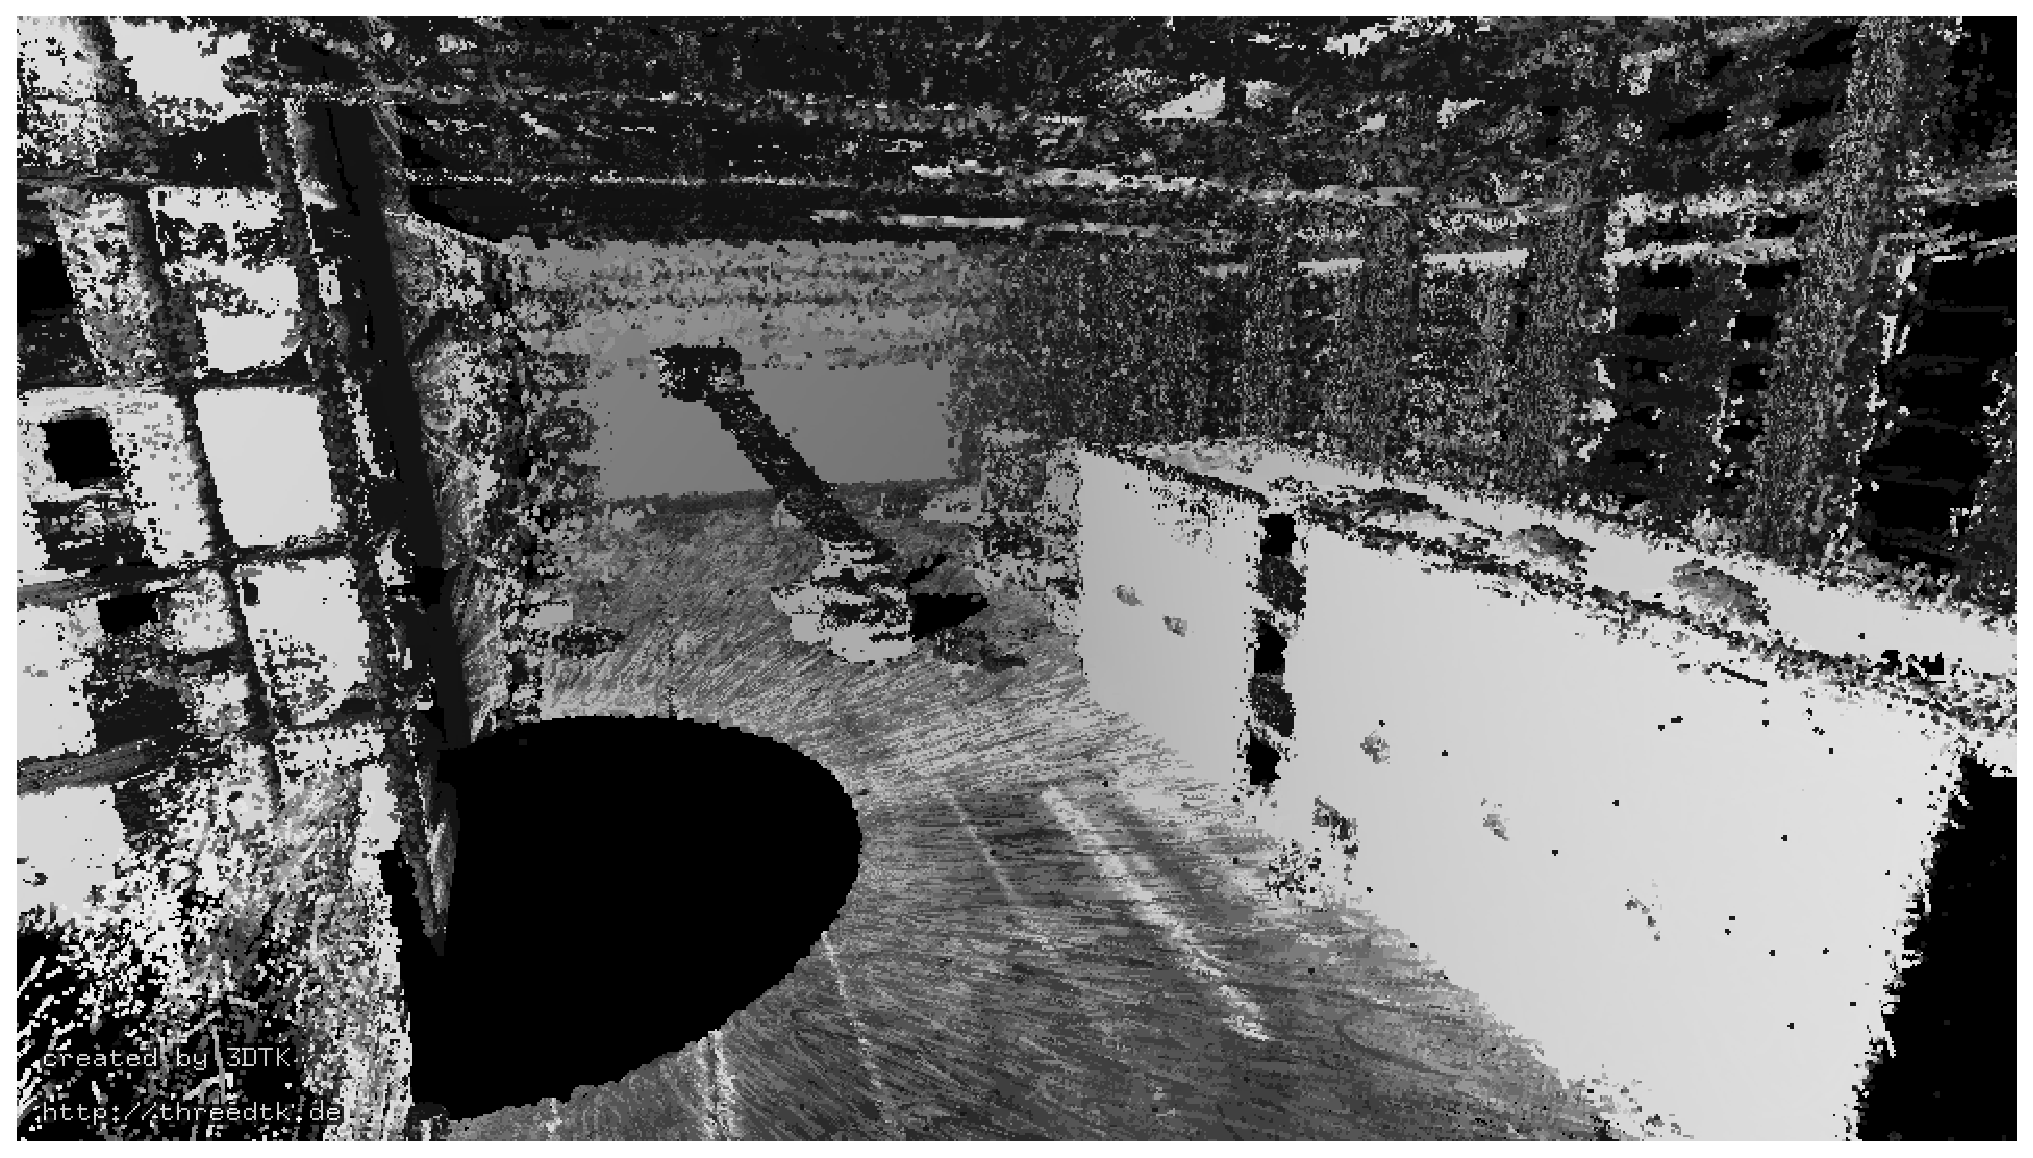
\includegraphics[width=\textwidth]{images/scan-sphere-fire}
	  	\end{minipage}\hfill
	  	\begin{minipage}[c]{0.2075\textwidth}
	  		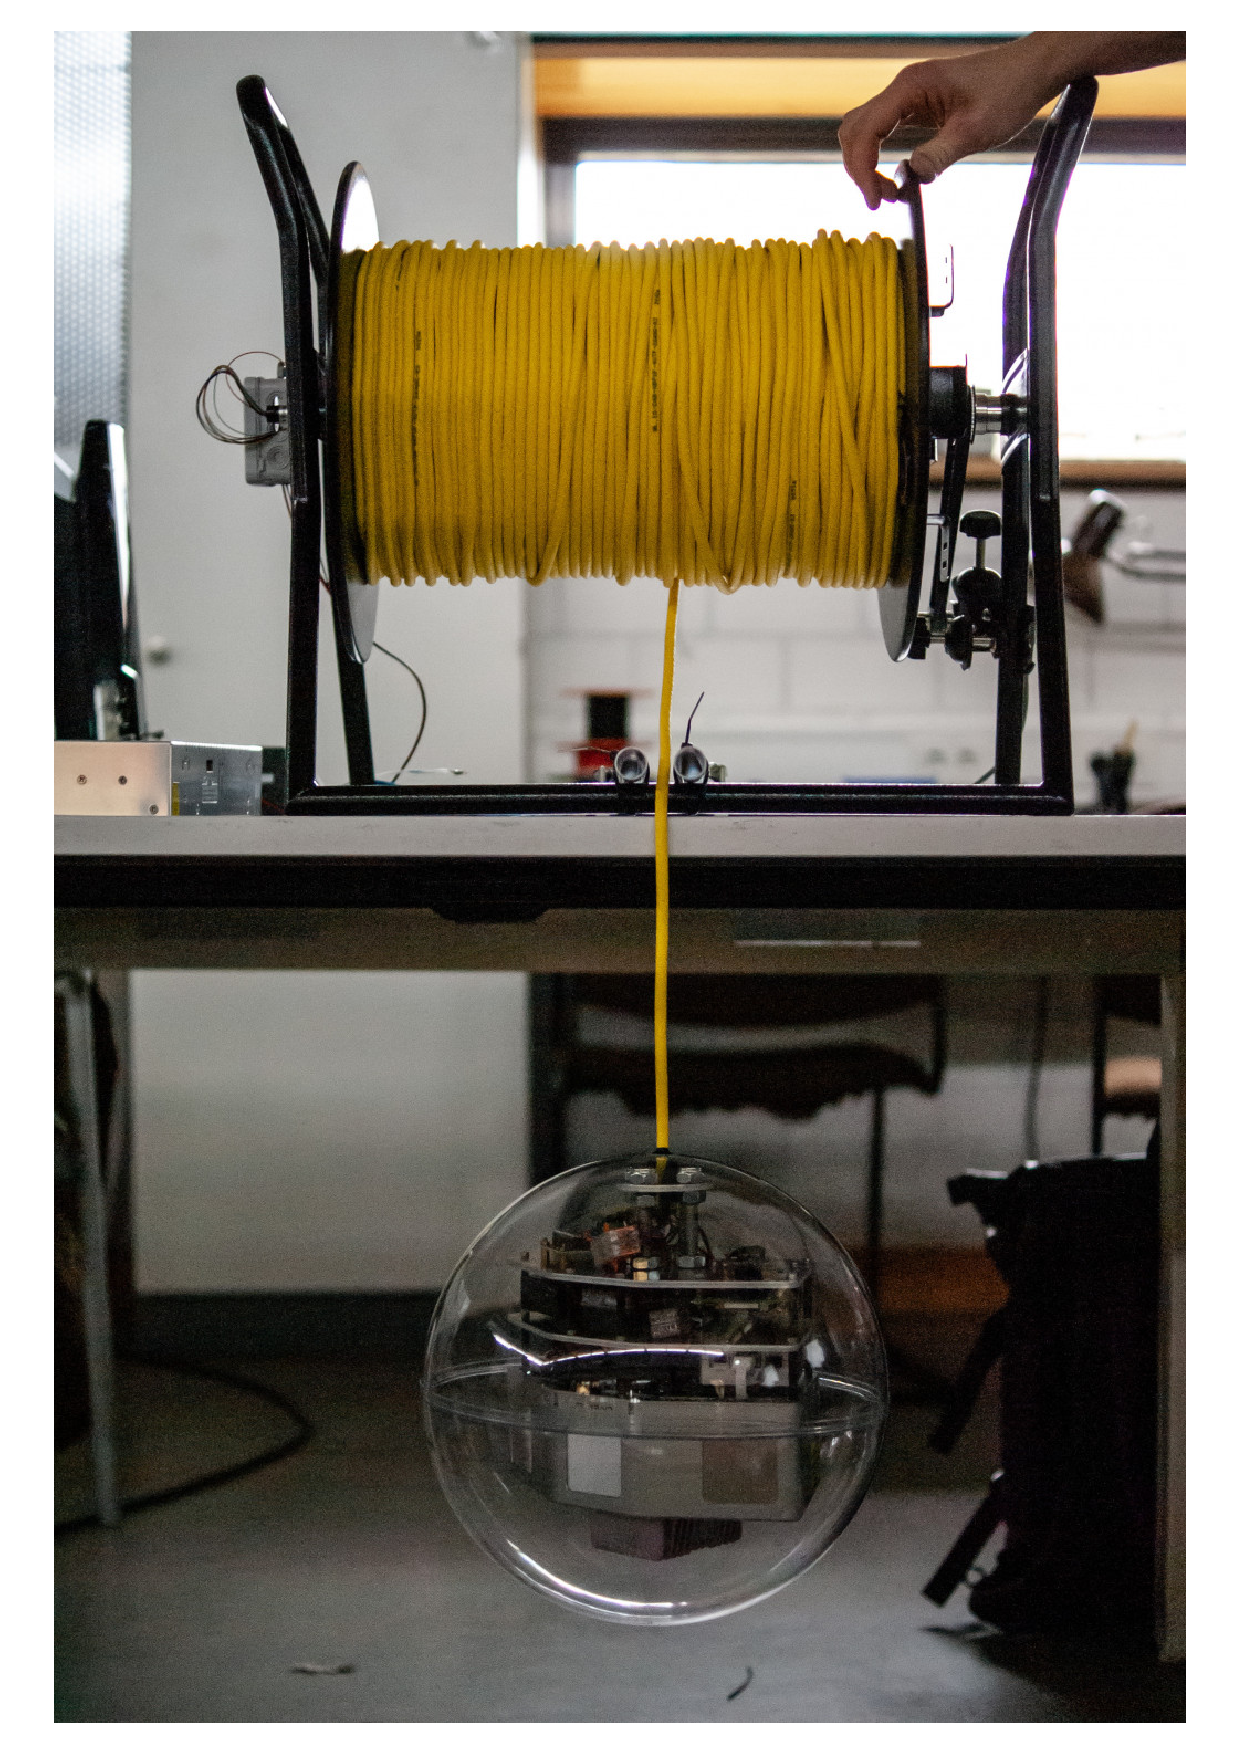
\includegraphics[width=\textwidth]{./images/lidarsetup}
	  	\end{minipage}
		\caption{Reference 3D point cloud acquired with a RIEGL 3D terrestrial laser scanner (top left). The 3D point cloud acquired by the test sphere after the rigid registration (bottom left) and a picture of the test setup (right).}
		\label{fig:experimental-setup}
	\end{figure}
\fi



%!TEX root = ../main.tex
\section{Results}

\subsection{Simulated Results}

The plane-based registration is applied to the simulated dataset with noisy pose and range measurements (cf. Figure~\ref{fig:simulatedDatasets}) without further processing.
Assuming this represents a coarsely pre-registered 3D point cloud, the distances to the ground truth were evaluated before and after the plane-based registration. 
Figure~\ref{fig:simulatedEvaluation} shows the different point-to-point distances. 

\begin{figure*}
 	\centering
 	\begin{minipage}[c]{0.495\textwidth}
 		\centering
		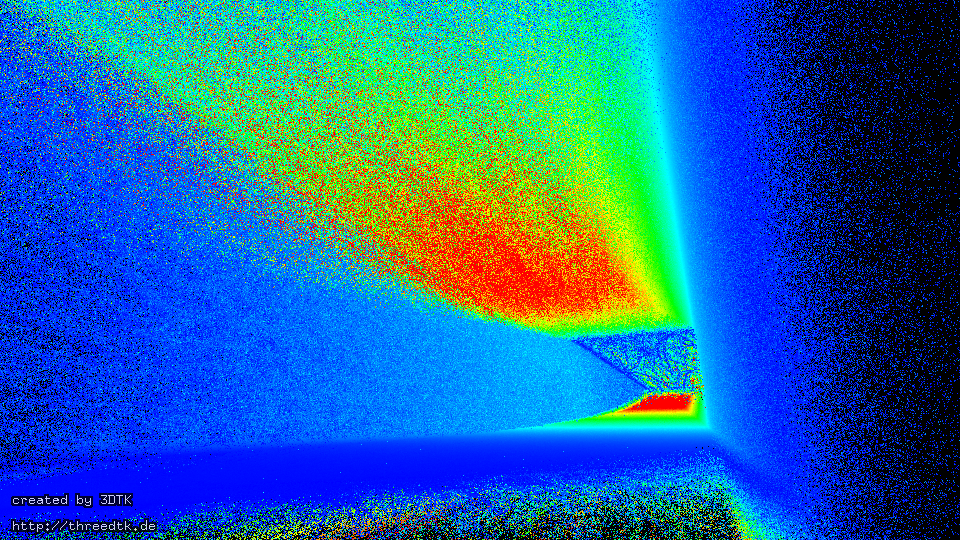
\includegraphics[width=\textwidth]{./images/uncorr_bottom_pose}\\
		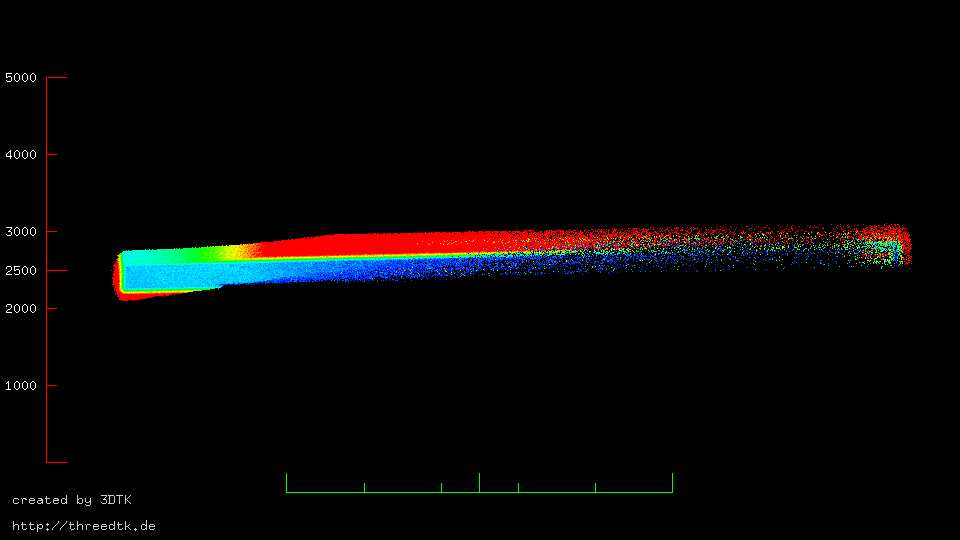
\includegraphics[width=\textwidth]{./images/uncorr_side_view}\\
  		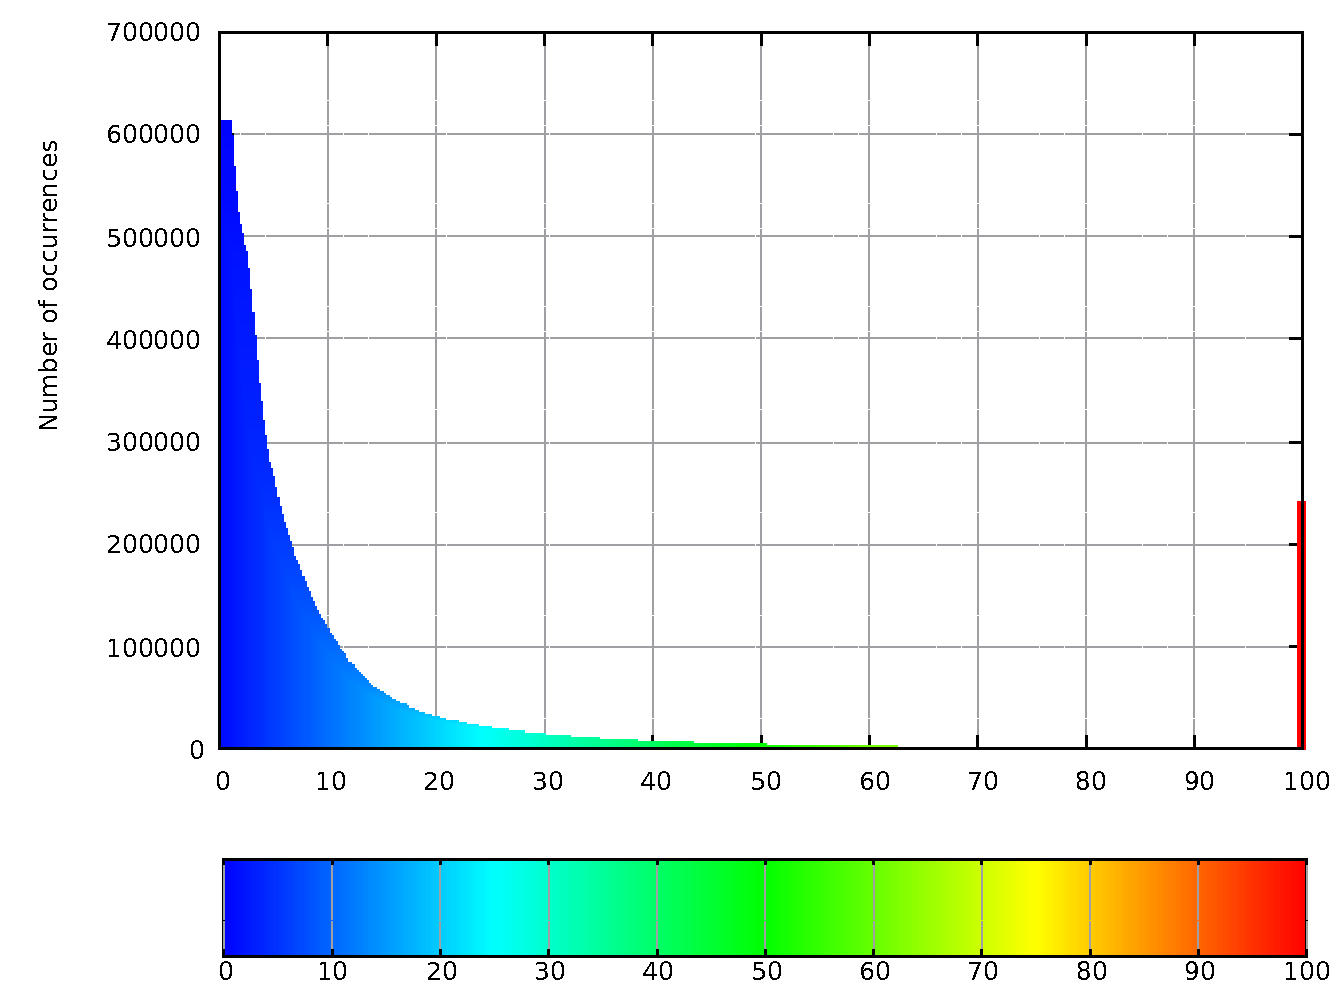
\includegraphics[width=\textwidth]{./images/uncorr_hist}
  	\end{minipage}\hfill
  	\begin{minipage}[c]{0.495\textwidth}
  		\centering
		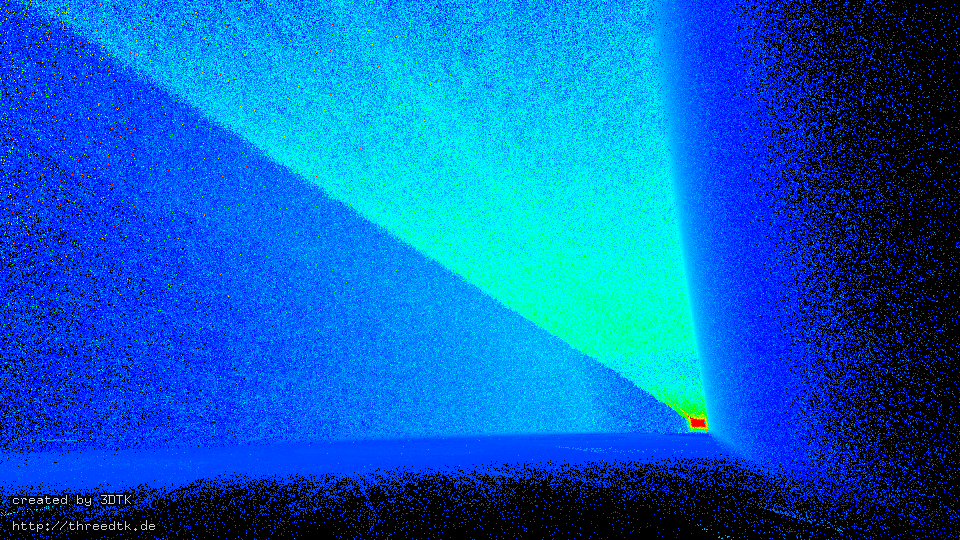
\includegraphics[width=\textwidth]{./images/corr_bottom_pose}\\
		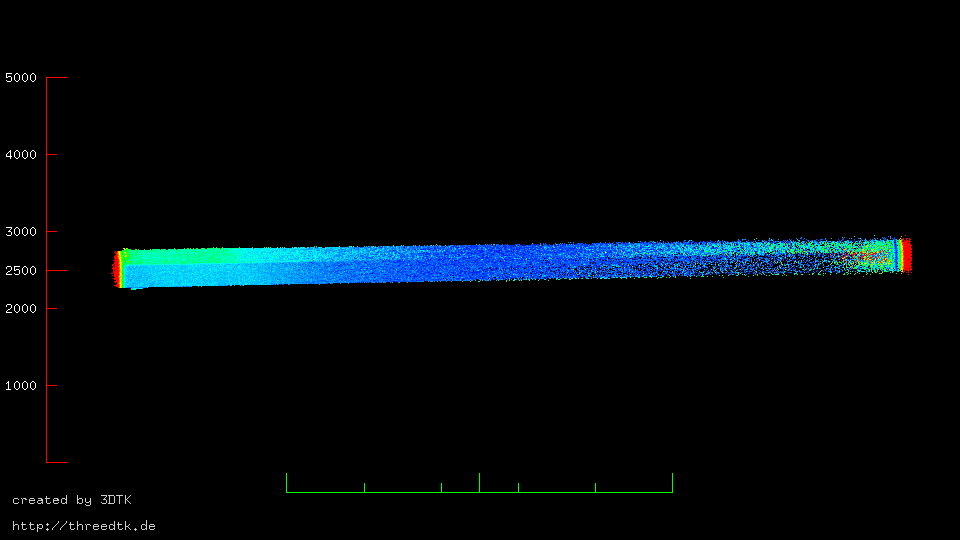
\includegraphics[width=\textwidth]{./images/corr_side_view}\\
  		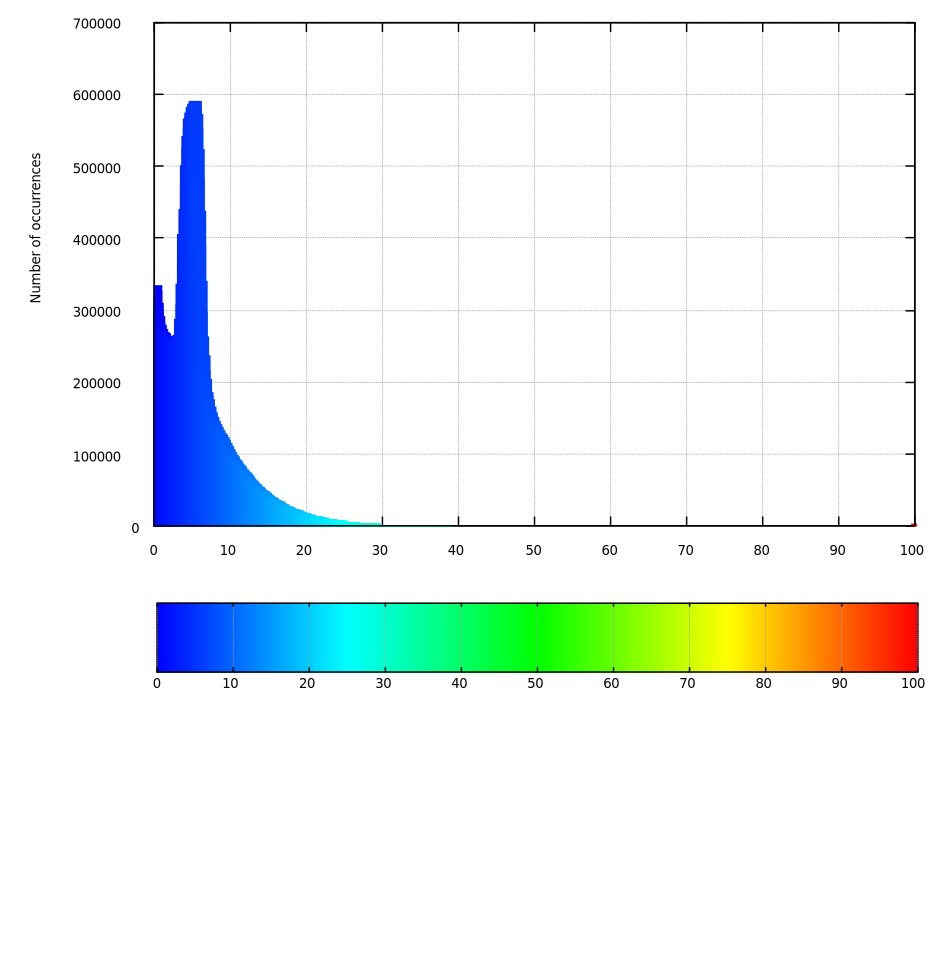
\includegraphics[width=\textwidth]{./images/corr_hist}
  	\end{minipage} 	
 	\caption{Evaluation of point distances before (left) and after (right) the plane-based registration on a simulated dataset. Lateral images always have the same orientation. A maximal distance of \SI{30}{m} is set, such that all points that display a higher distance value are excluded from the analysis. Both point-clouds were reduced before evaluating point-to-point distances to the ground-truth. Further, the color-space maps all values with a distance greater than \SI{1}{m} to the same color. The top two columns show a heat map of distances, while the bottom shows the corresponding histogram. The color mapping is equivalent in both. An animation of the matching process is given at \url{https://youtu.be/7igQdEeCsYk}.} 
 	\label{fig:simulatedEvaluation}
\end{figure*} 

Before the registration, the corridor is only represented acceptably in the front part. 
The further into the corridor, i.e., the longer the robot accumulates errors, the more imprecise the data becomes. 
Finally, we see that many points exceed the threshold of \SI{1}{\meter} and thus being mapped to the same color value.
After registration, we see that, qualitatively, the ideal corridor was nearly restored from the noisy data. 
In particular a very large portion of points (90\%) have distances of less than \SI{35.9}{\centi\meter}.
Table~\ref{tab:percentiles} shows the comparison of further percentiles of both datasets. 

\begin{table}
	\centering
	\begin{tabular}{@{}lccc@{}}\hline
		& P90 & P95 & P98 \\ \hline\hline
		Uncorrected & \SI{372.1}{\centi\meter} &  \SI{553.4}{\centi\meter} &  \SI{827.9}{\centi\meter} \\%& \SI{9.7}{\centi\meter}\\
		Corrected & \SI{35.9}{\centi\meter} &  \SI{64.1}{\centi\meter} &  \SI{122.8}{\centi\meter} \\\hline%& \SI{6.3}{\centi\meter}\\ \hline
	\end{tabular}
	\caption{Comparison of point-distances in the uncorrected and corrected simulated dataset.}
	\label{tab:percentiles}
\end{table}

Further, the square and straight shape of the corridor is restored well, and especially the large amount of points with an errors of greater than \SI{1}{m} is removed. 
Any such errors tend to occur at the back and the front of the corridor where the measured range is the largest hence has the largest contribution of the range error. 

\subsection{Floating Sphere Results}

Figure~\ref{fig:cylon-corrected} shows the results obtained before and after employing the plane based registration on the dataset acquired by the floating sphere.
The pre-registration is obtained by determining the orientation of the sphere via Madgwick filtered~\cite{madgwick2010efficient} IMU measurements.
To increase the number of possible point-to-plane correspondences we combine twenty temporally successive scans into one meta-scan, which is then globally registered. 
We always use the scan at the median index as a reference coordinate system.
This does not only speed up convergence due to the proportional effect on the error function but also decreases the risk of transforming a single line scan incorrectly.
Transformations like these happen in particular for a small collection of points as outliers have more influence.

\begin{figure*}
	\centering
	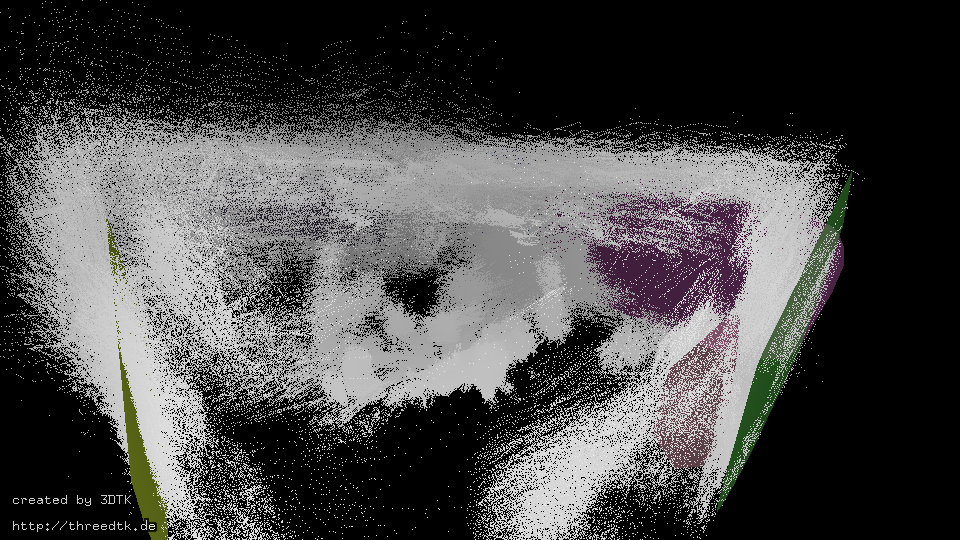
\includegraphics[width=0.495\textwidth]{./images/cylon_uncorr_corner}\hfill
	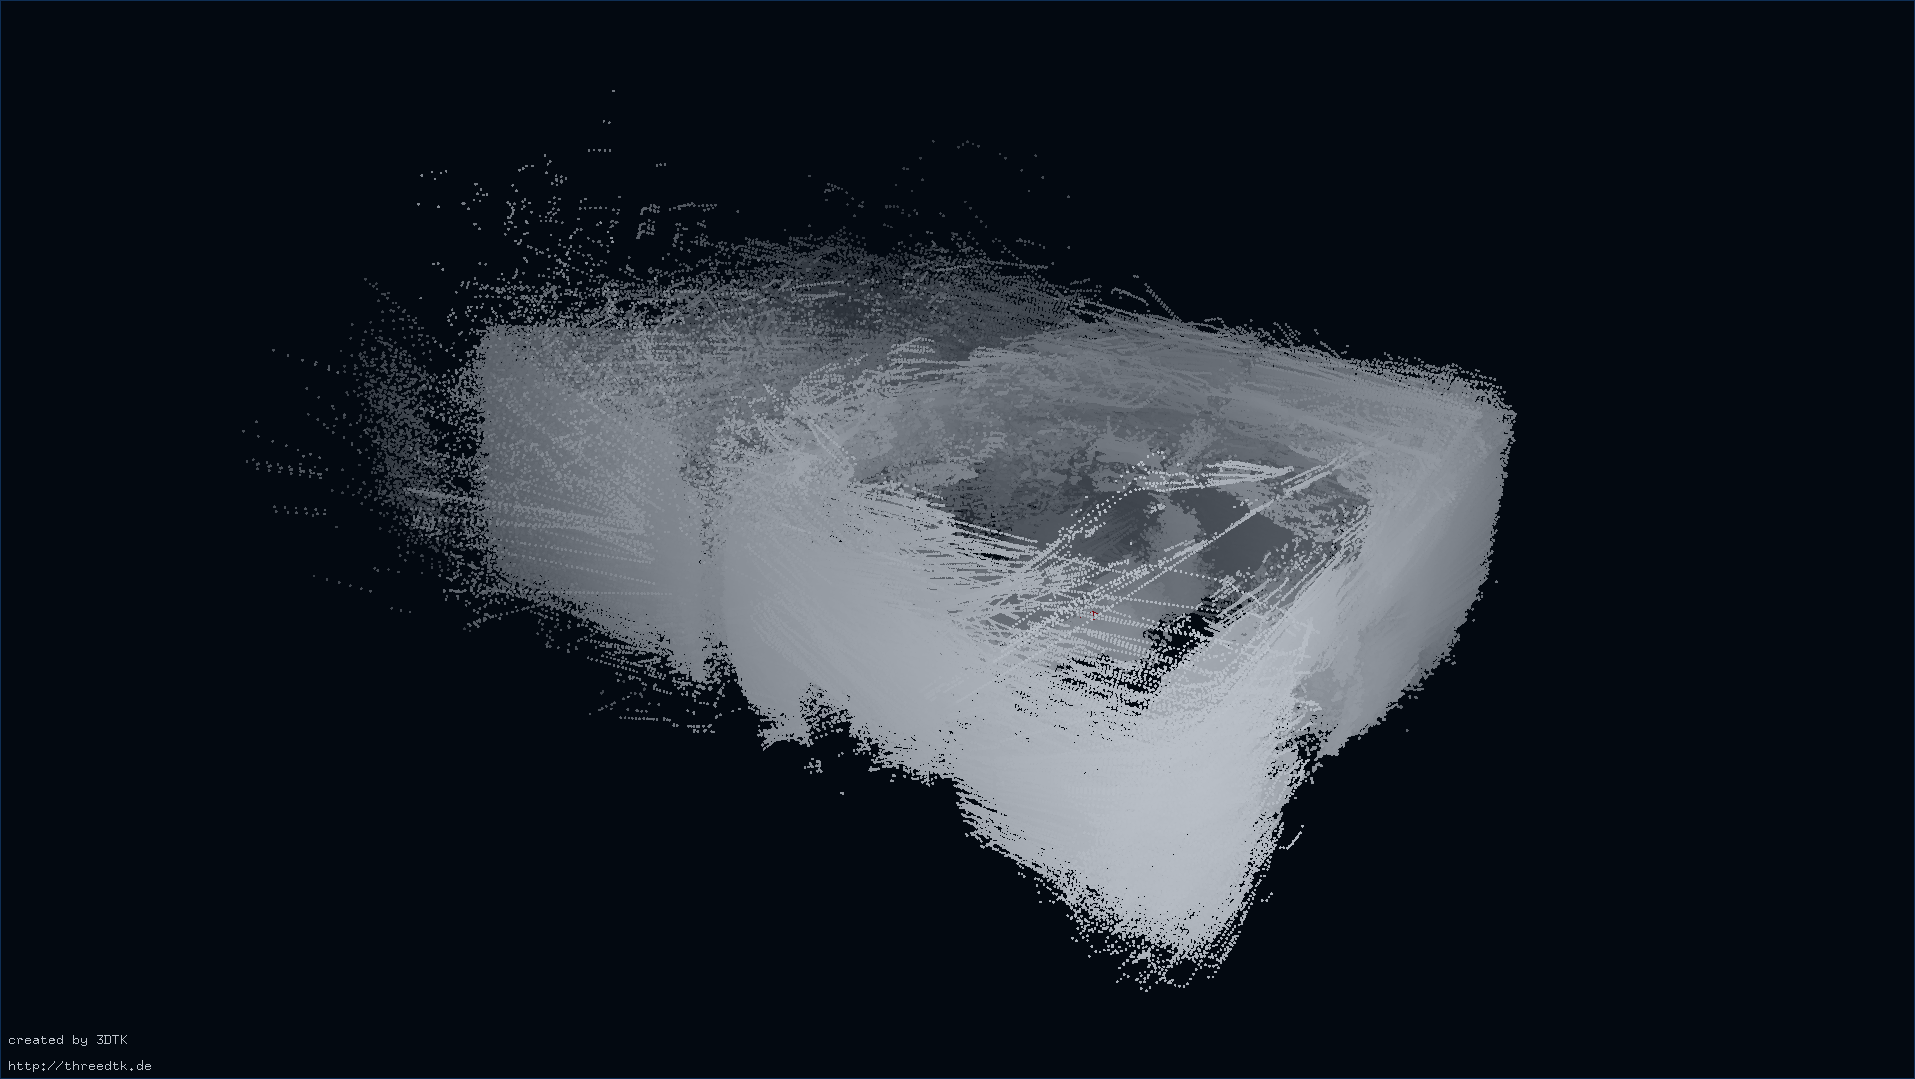
\includegraphics[width=0.495\textwidth]{./images/cylon_corr_corner}\\
	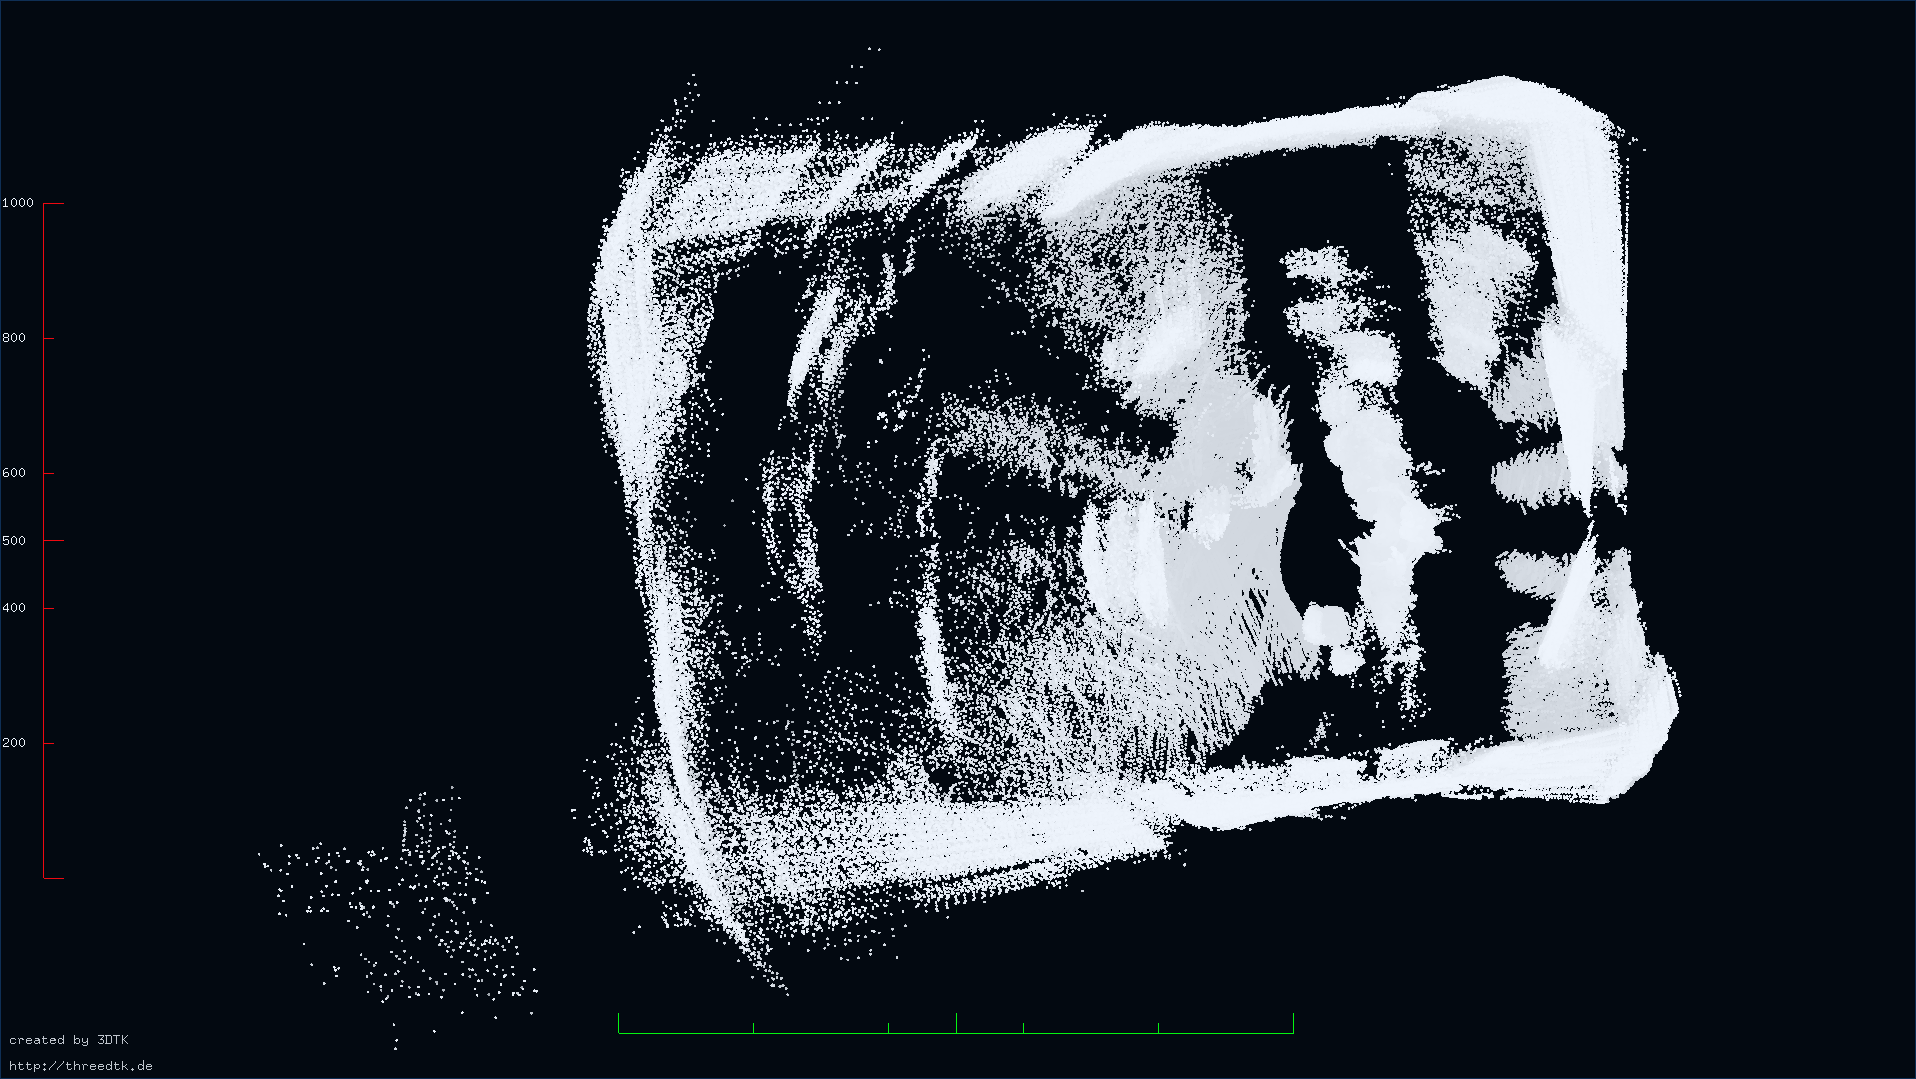
\includegraphics[width=0.495\textwidth]{./images/cylon_uncorr_top}\hfill
	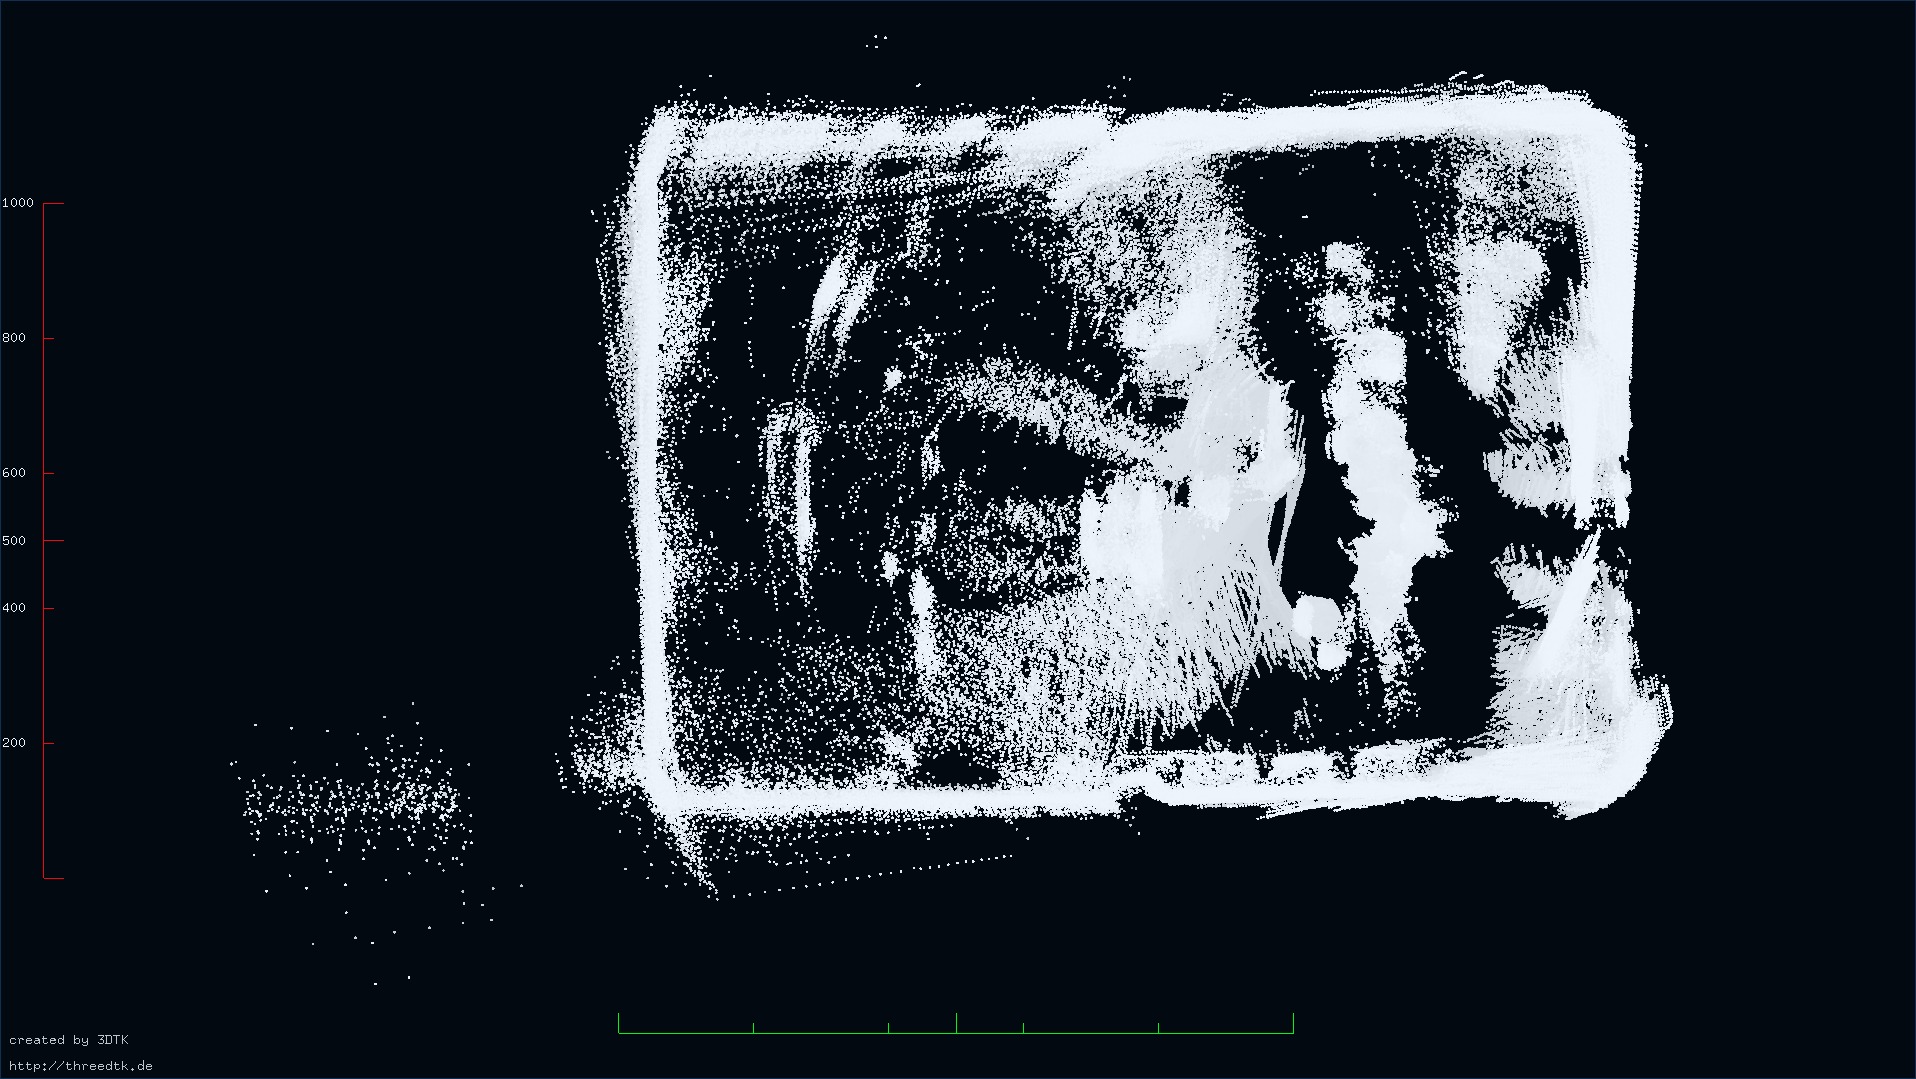
\includegraphics[width=0.495\textwidth]{./images/cylon_corr_top}
	\caption{The point cloud acquired by the floating sphere before (left) and after (right) applying the plane based registration. View from the interior (top) and a birds-eye view (bottom). Parameters used for optimization: $\epsilon_H = 50$, $\epsilon_P = 200$, $\epsilon_\alpha = \frac{\pi}{4}$, $K = 20$ for AKNN, $d_{growth} = 50$, $N_{c_min} = 200$, $\alpha_0 = [0.01, 0.01, 0.01, 0, 0, 0]^\tau$, $i = 8$, $k = 100$. An animation of the registration process is given at \url{https://youtu.be/Qa2Qi8z0KEk} .}
	\label{fig:cylon-corrected}
\end{figure*}
After the registration, the walls of the room are significantly more prominent in the point cloud. 
In particular, the noise in the top left corner of the top view (cf. figure~\ref{fig:cylon-corrected}) has been visibly reduced.
Further, the deviation of points around the walls is notably smaller as the points are moved on the plane.

\subsection{Rolling Sphere Results}

Figure~\ref{fig:jasperhome} shows the results obtained before and after employing the presented algorithm on the dataset, acquired by the prototype in figure~\ref{fig:prototype}.
We again combine twenty temporally successive scans into one meta-scan, using the scan at the median index as a reference coordinate system, which is then globally registered.
We used the first seven of these meta-scans, corresponding to the first full rotation of the spher, to extract global planes.
All subsequent meta-scans are then matched against the initial global plane model.
We use both optimizations from section \ref{ssec:furtheropts}, introducing a global up/down lock for gradient descent and applying sequential iteration to eliminate accumulating pose error.


\begin{figure*}
        \centering
        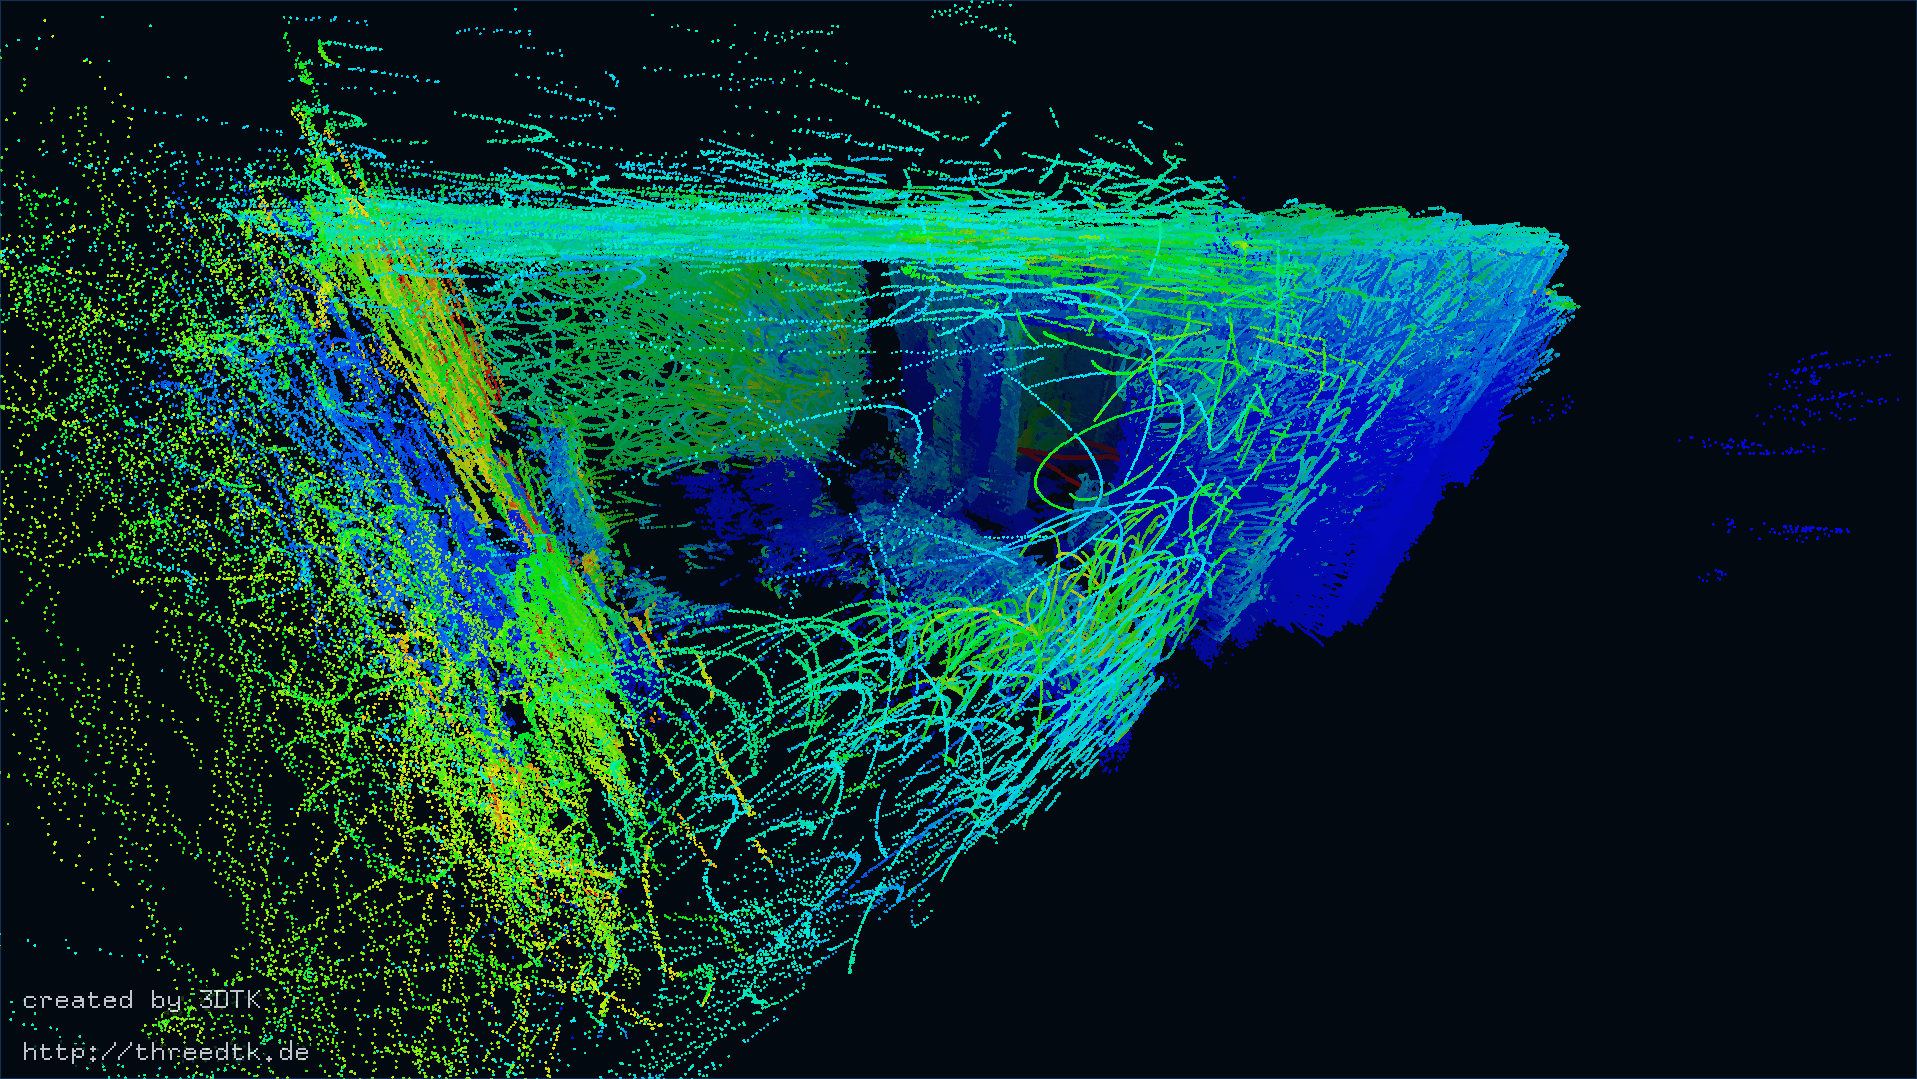
\includegraphics[width=0.495\textwidth]{./images/jasper_uncorr_corner}\hfill
        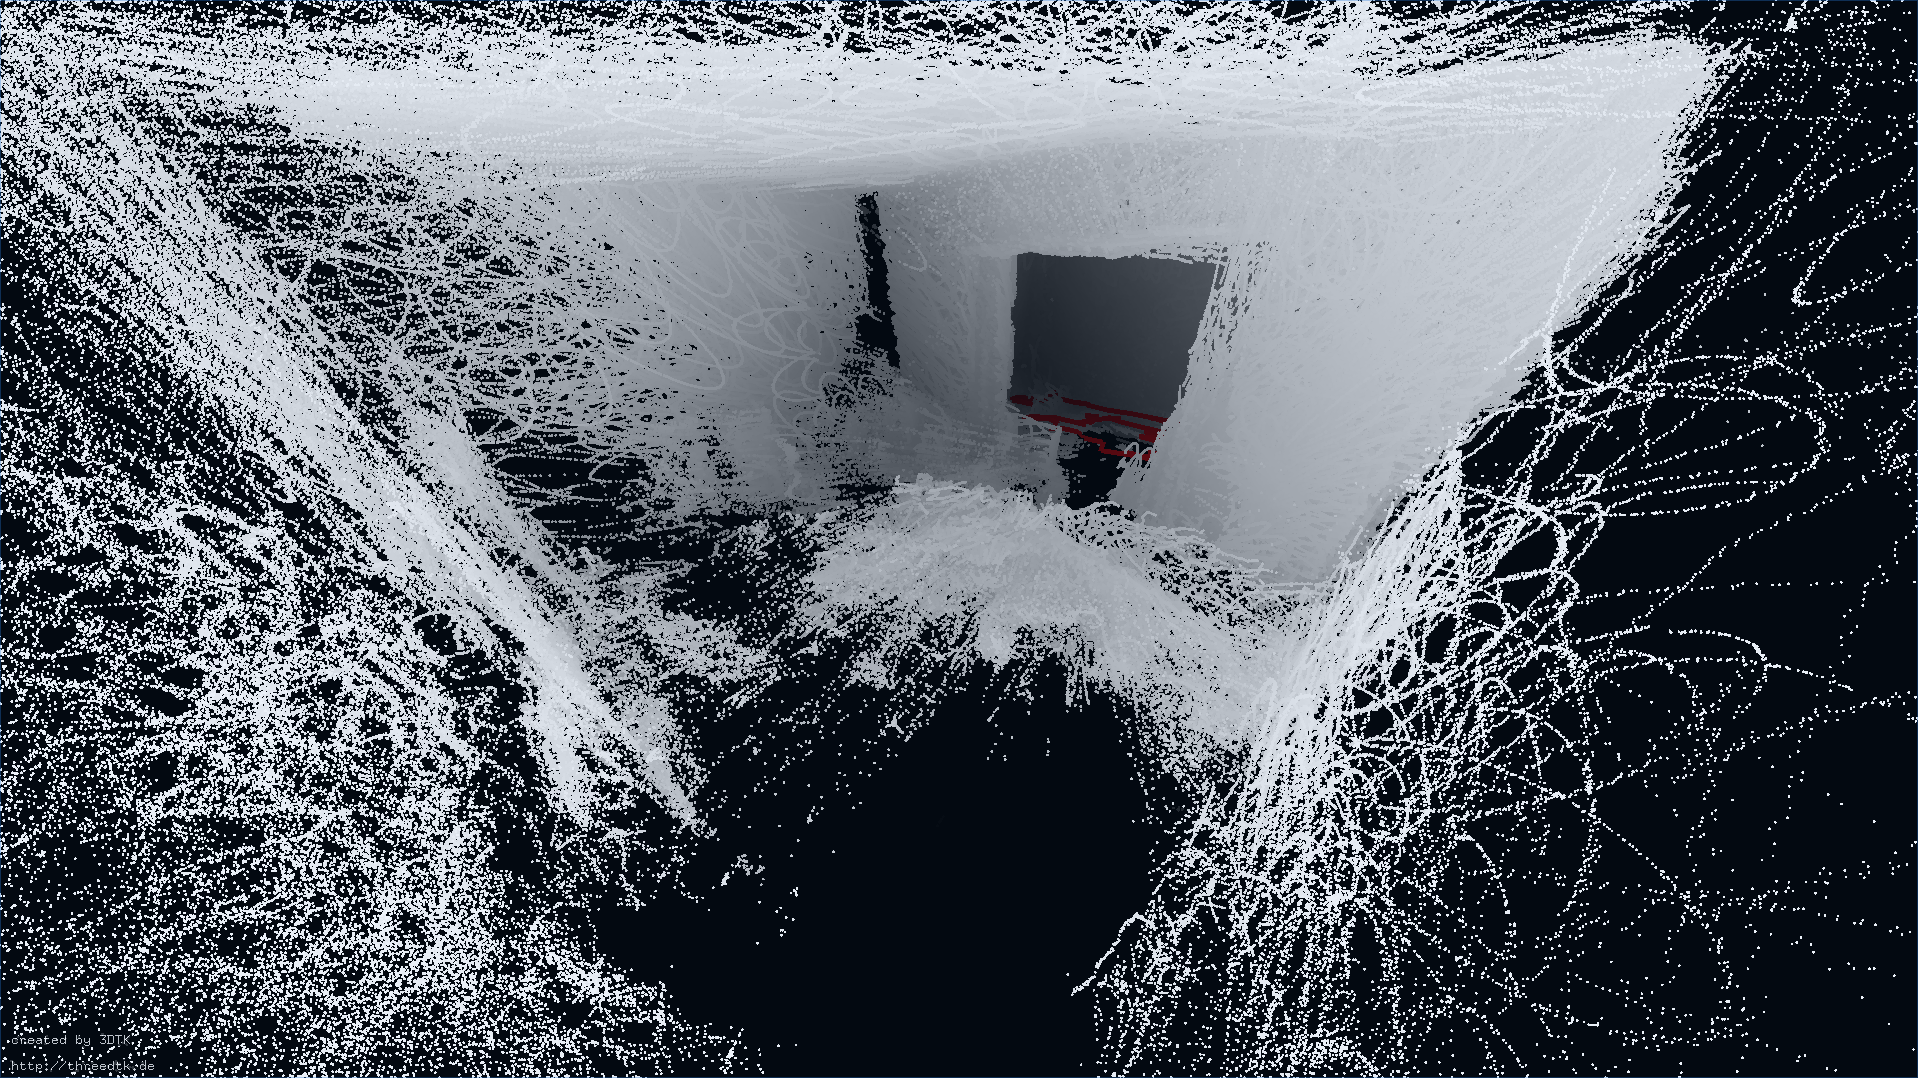
\includegraphics[width=0.495\textwidth]{./images/jasper_corr_corner}\\
	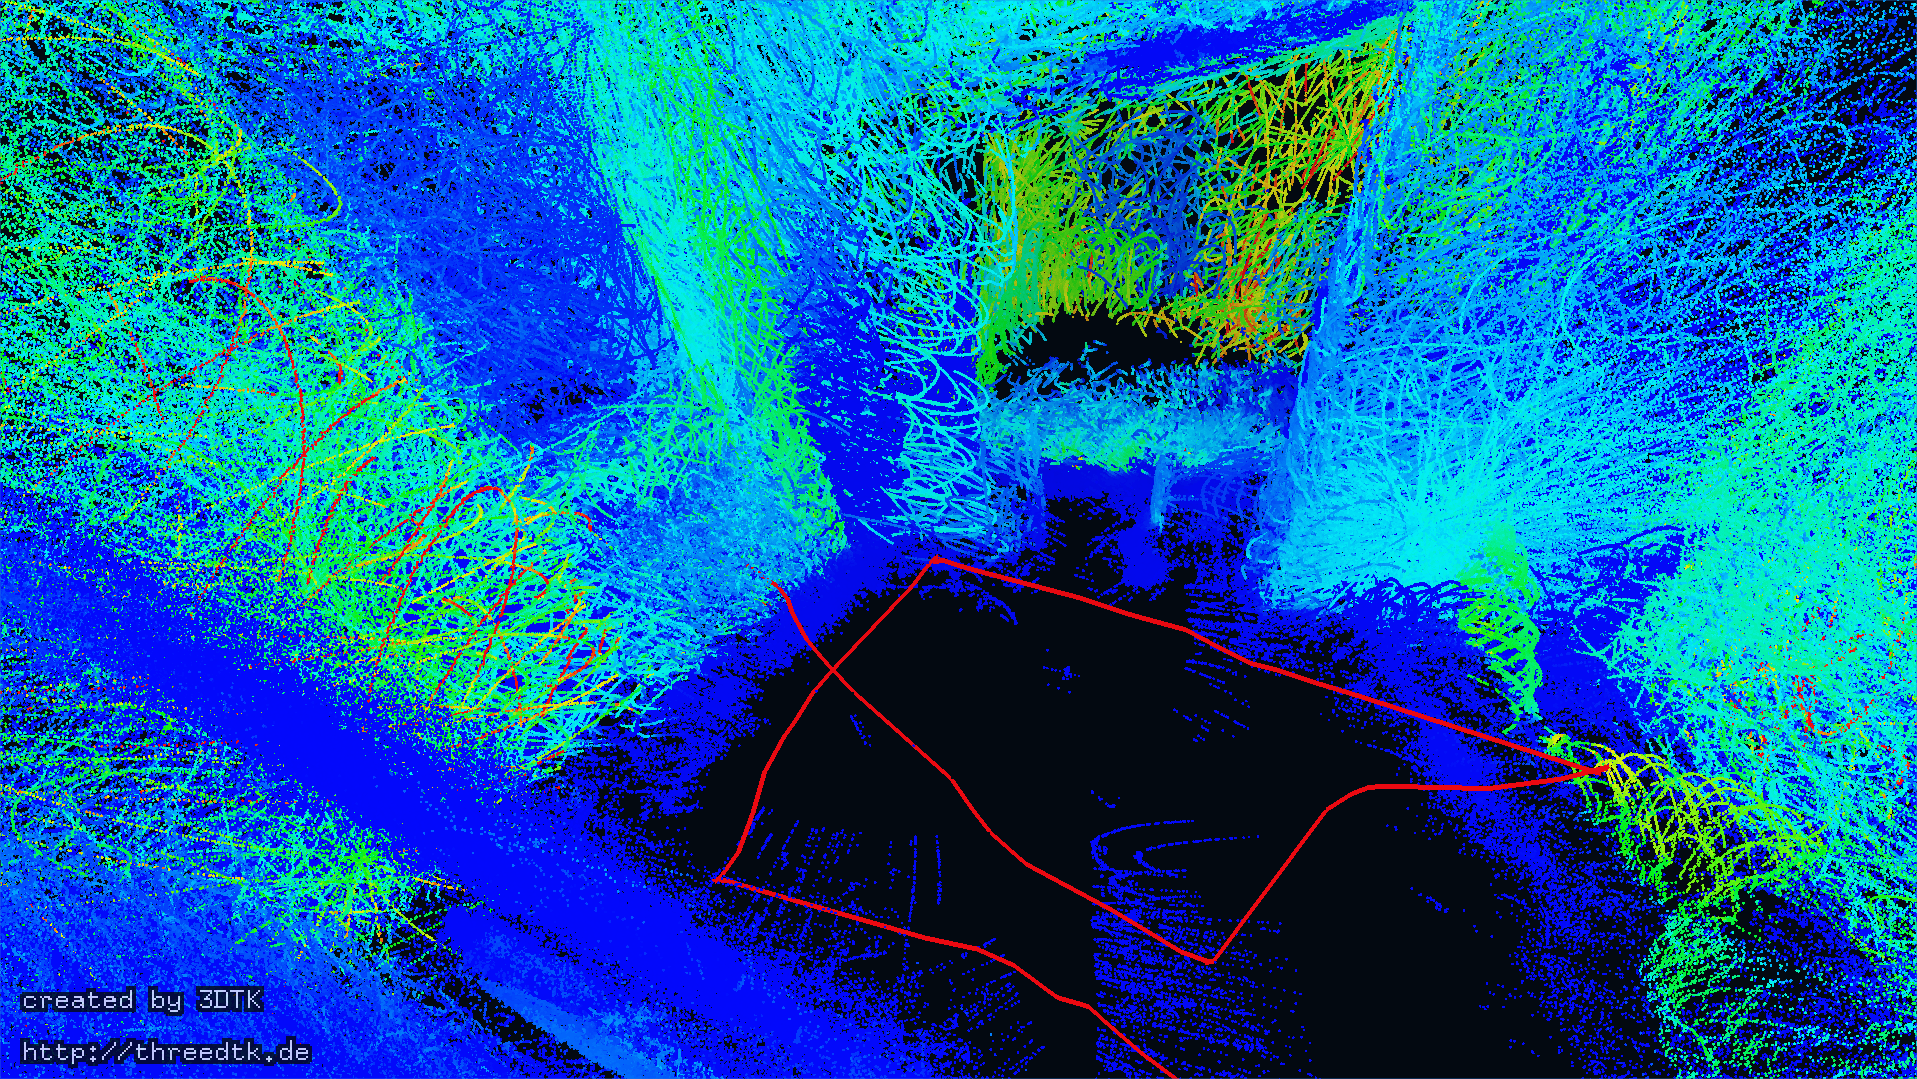
\includegraphics[width=0.495\textwidth]{./images/jasper_uncorr_color}\hfill
	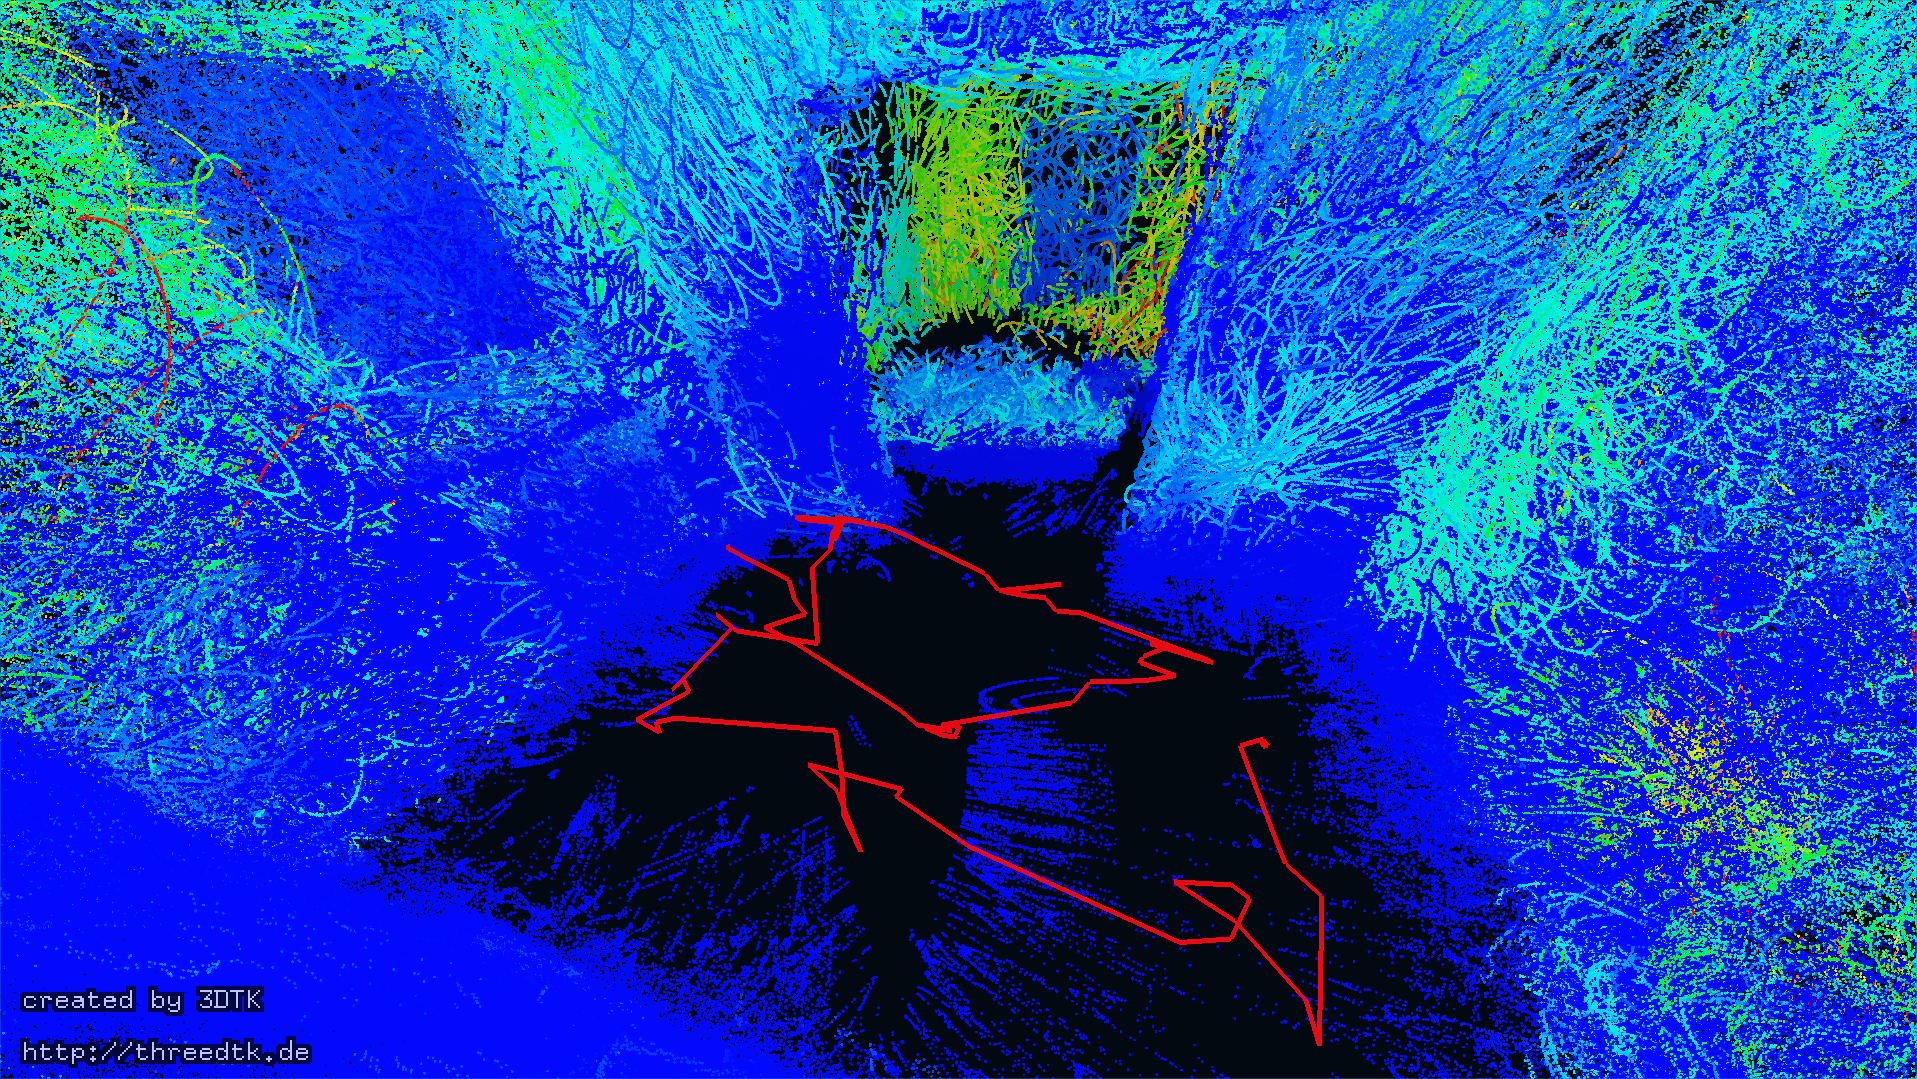
\includegraphics[width=0.495\textwidth]{./images/jasper_corr_color}\\
        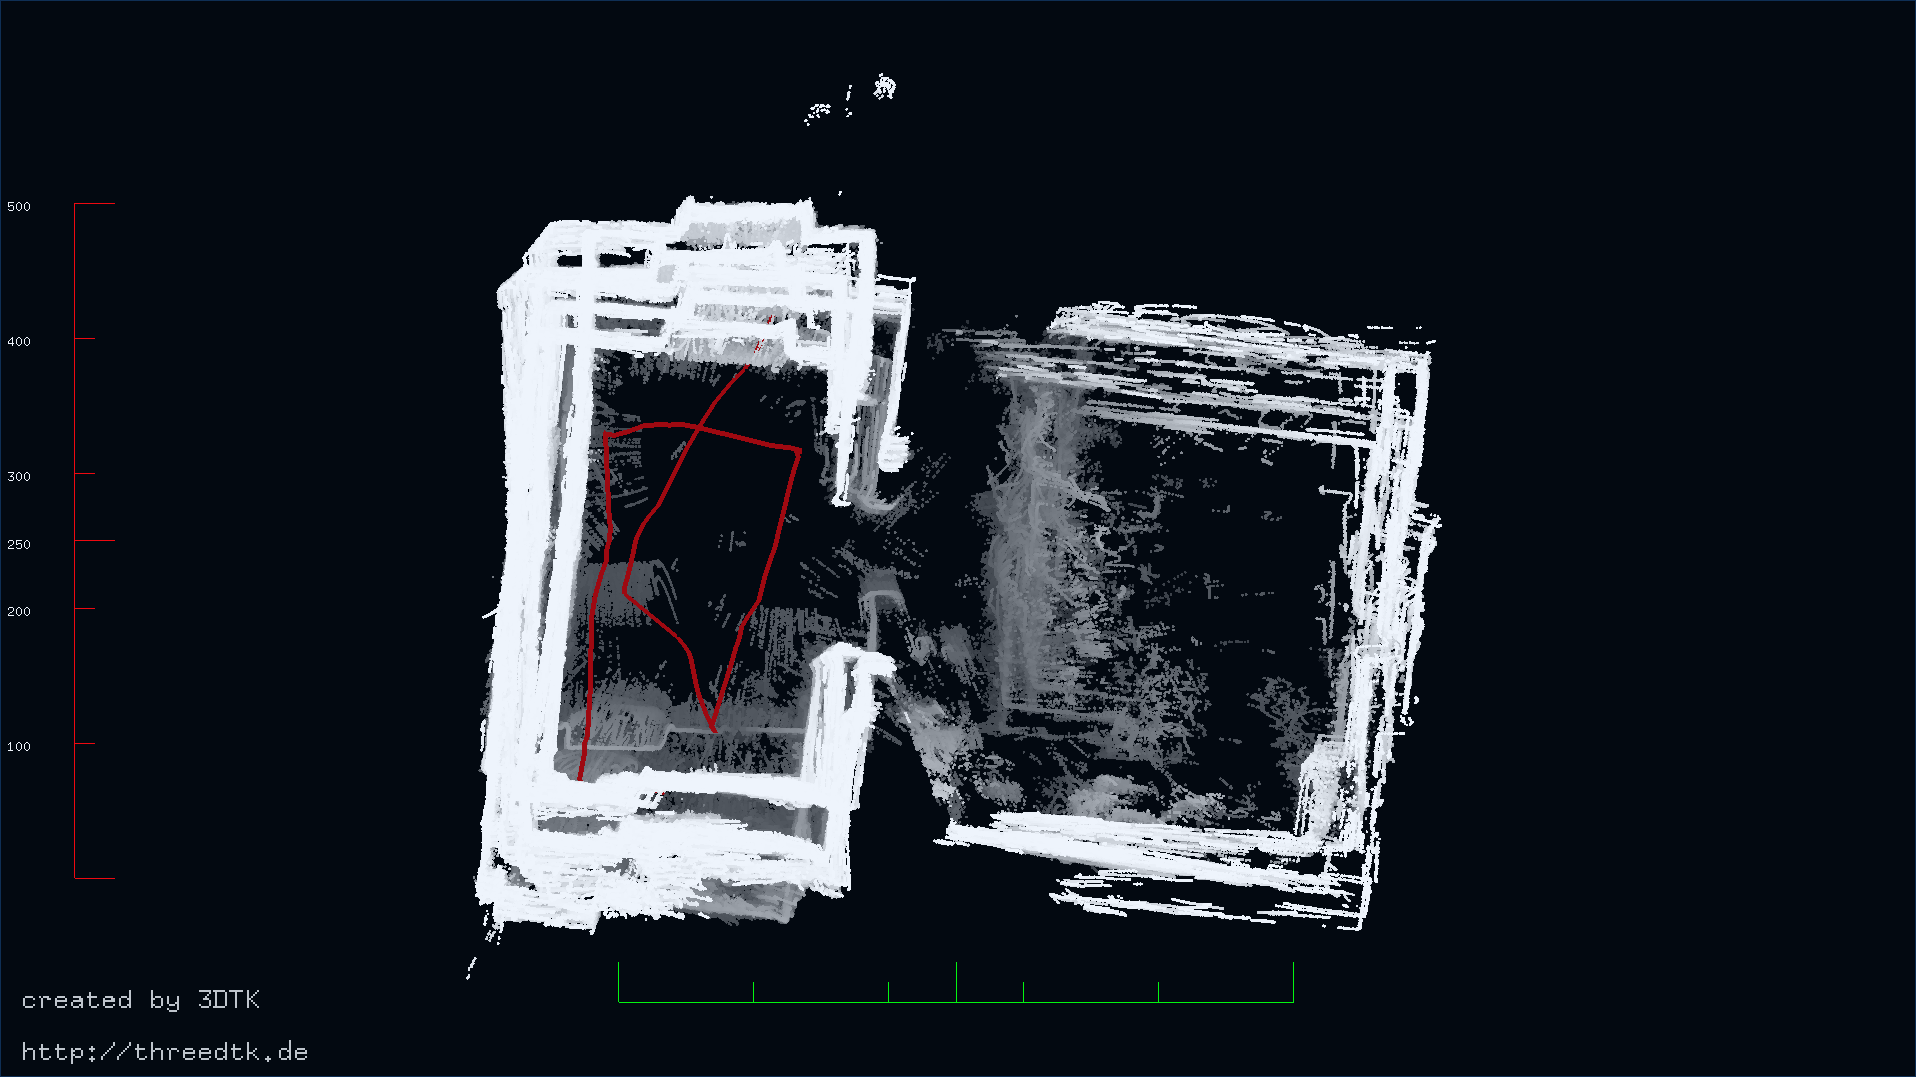
\includegraphics[width=0.495\textwidth]{./images/jasper_uncorr_top}\hfill
        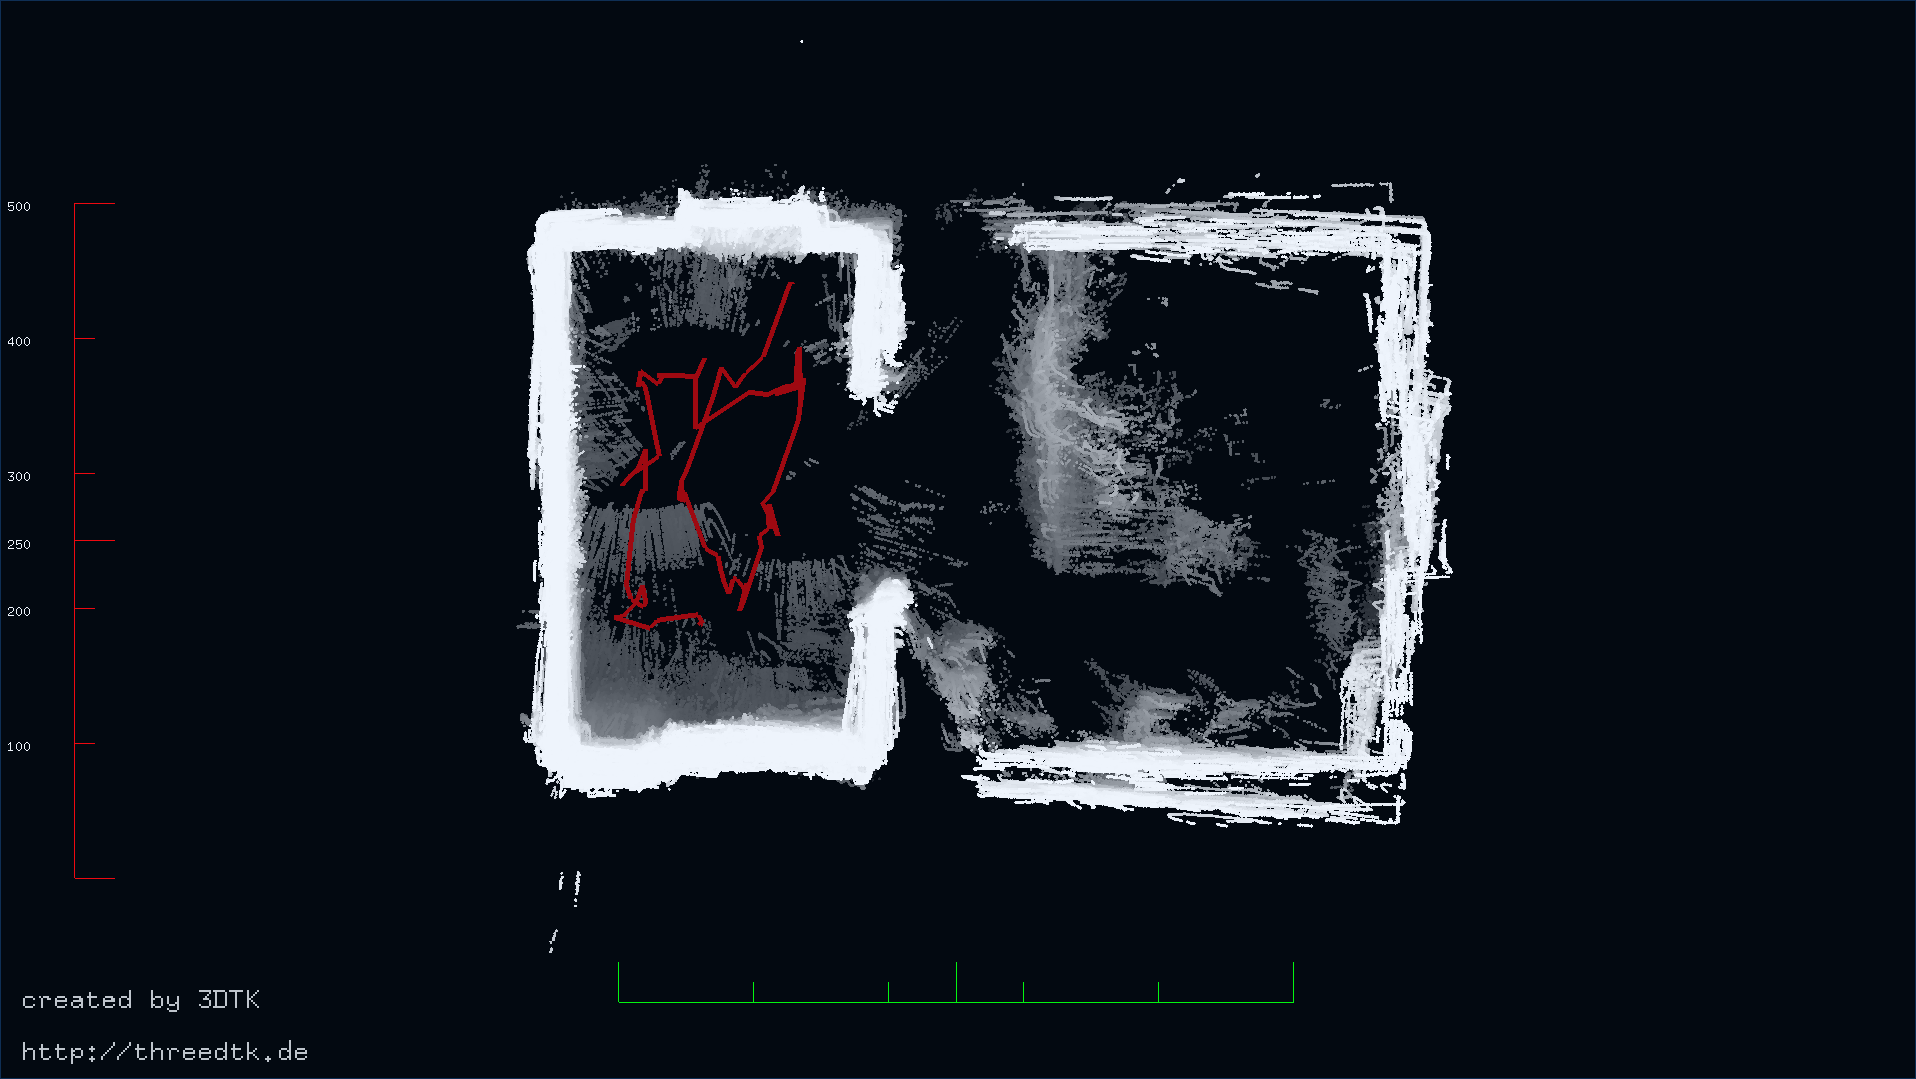
\includegraphics[width=0.495\textwidth]{./images/jasper_corr_top}
        \caption{The point cloud acquired by the rolling sphere before (left) and after (right) applying the plane based registration. View from the interior (top) and a birds-eye view (bottom). Parameters used for optimization: $\epsilon_H = 200$, $\epsilon_P = 300$, $\epsilon_\alpha = \frac{\pi}{4}$, $K = 200$ for AKNN, $d_{growth} = 50$, $N_{c_min} = 800$, $\alpha_0 = [0.001, 0.001, 0.001, 1, 0, 1]^\tau$, $i = 1500$, $k = 1$. An animation of the registration process is given at \url{https://youtu.be/hYR3xLhIdsE}.}
        \label{fig:jasperhome}
\end{figure*}
After the registration, the walls of the environment are no longer ambiguous, since all the subsequent scans are matched with the initial plane representation.
When considering the resulting path, it looks distorted.
This is because for some scans, especially empty ones where the sensor points to the ground, no planar features got matched with the global plane model, thus their pose is not optimized.
Improving the path quality is an objective for future works.

% This section is commented out
\iffalse
	\subsection{RADLER Results}

	\subsection{Experimental Results REMOVE THIS SECTION}

	For the experimentally acquired datasets a similar procedure is followed. 
	The main difference being, that the scan was pre-registered using a point-to-point based method as described in section~\ref{sec:experimentalSetup}. 
	Here also the point distances to the ground truth (in this case the terrestrially acquired 3D laser scan) is evaluated before and after the plane-based registration process. 

	\begin{figure}
		\centering
		\begin{minipage}[c]{0.25\textwidth}
			\centering	
			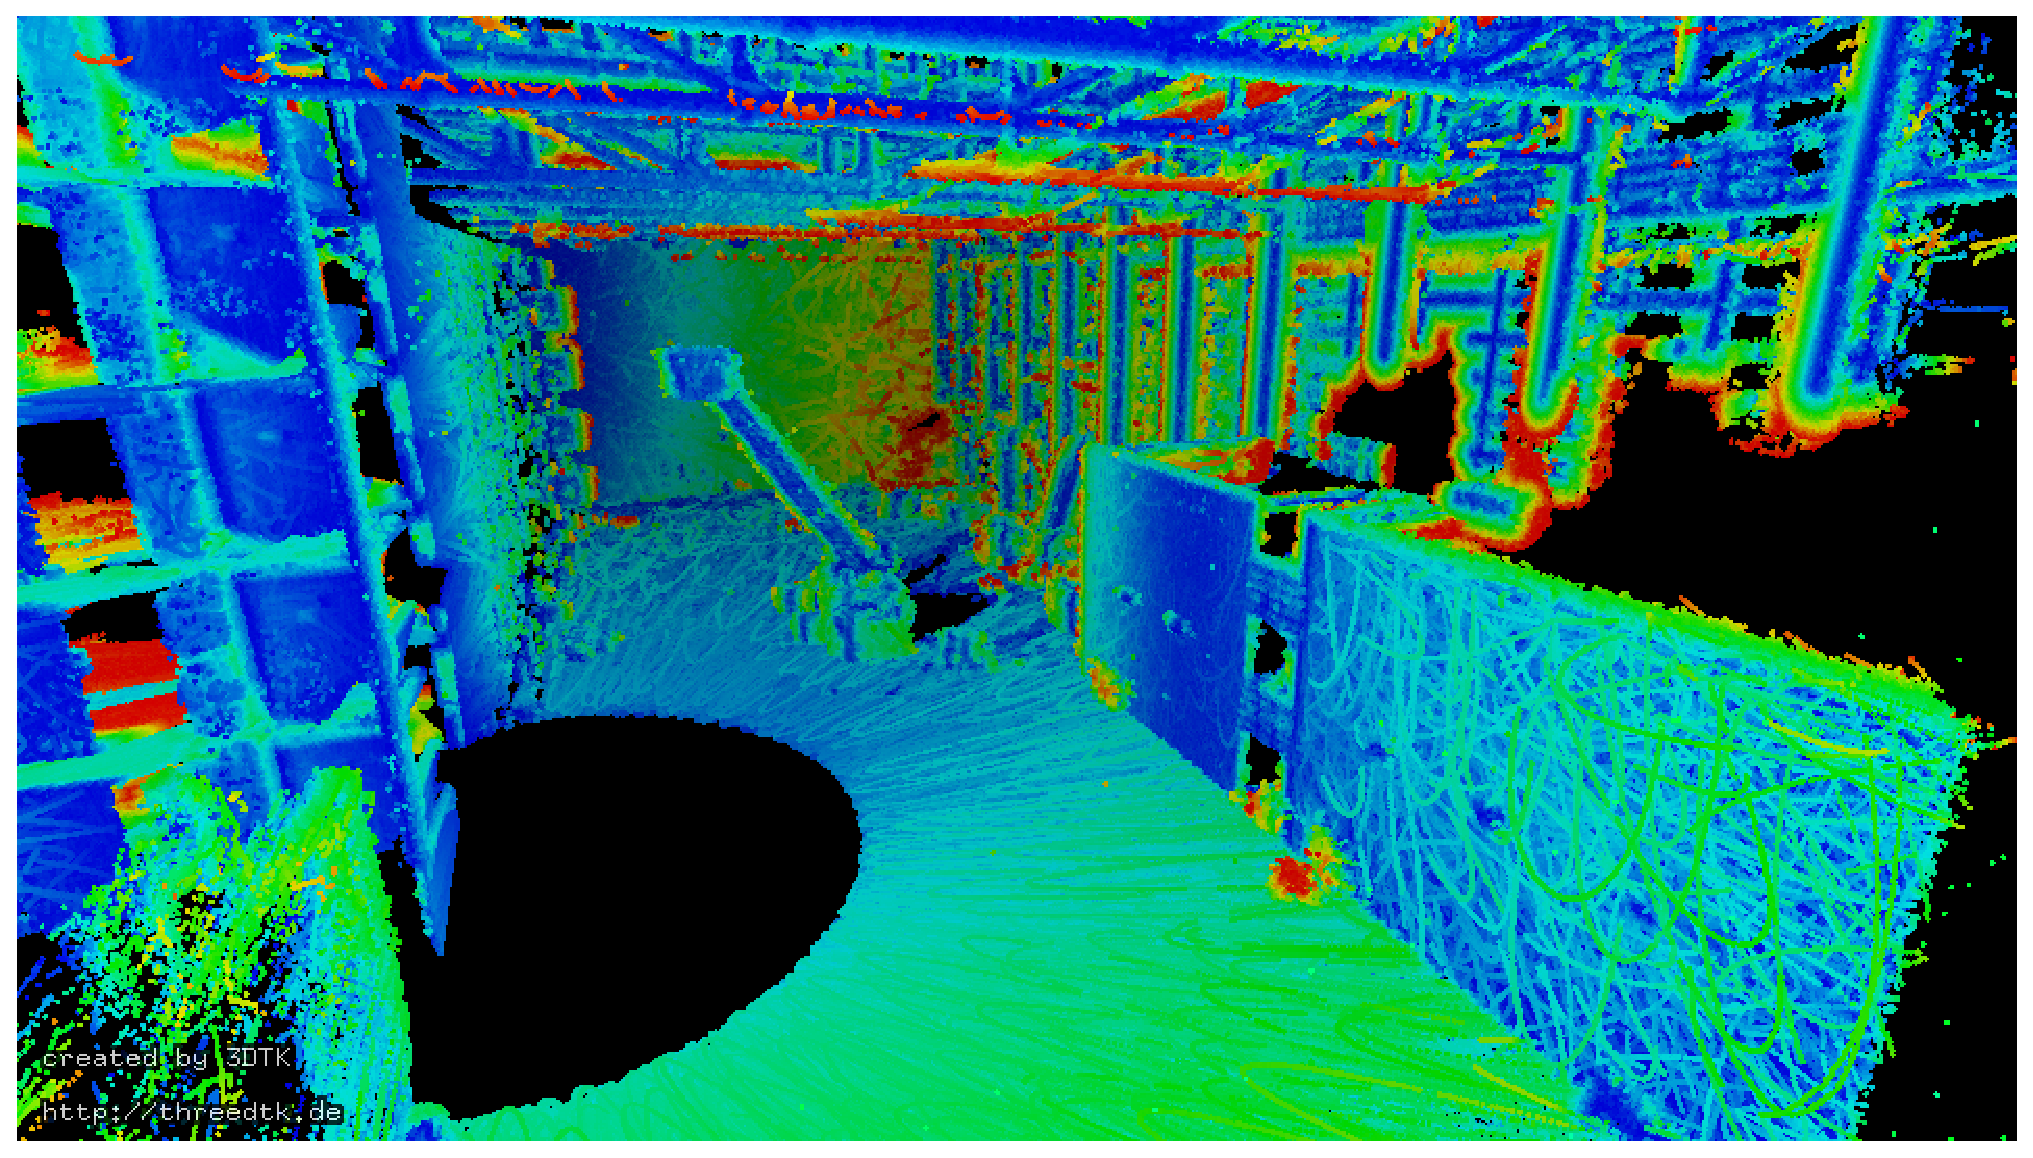
\includegraphics[width = \textwidth]{./images/distances_fire}\\
			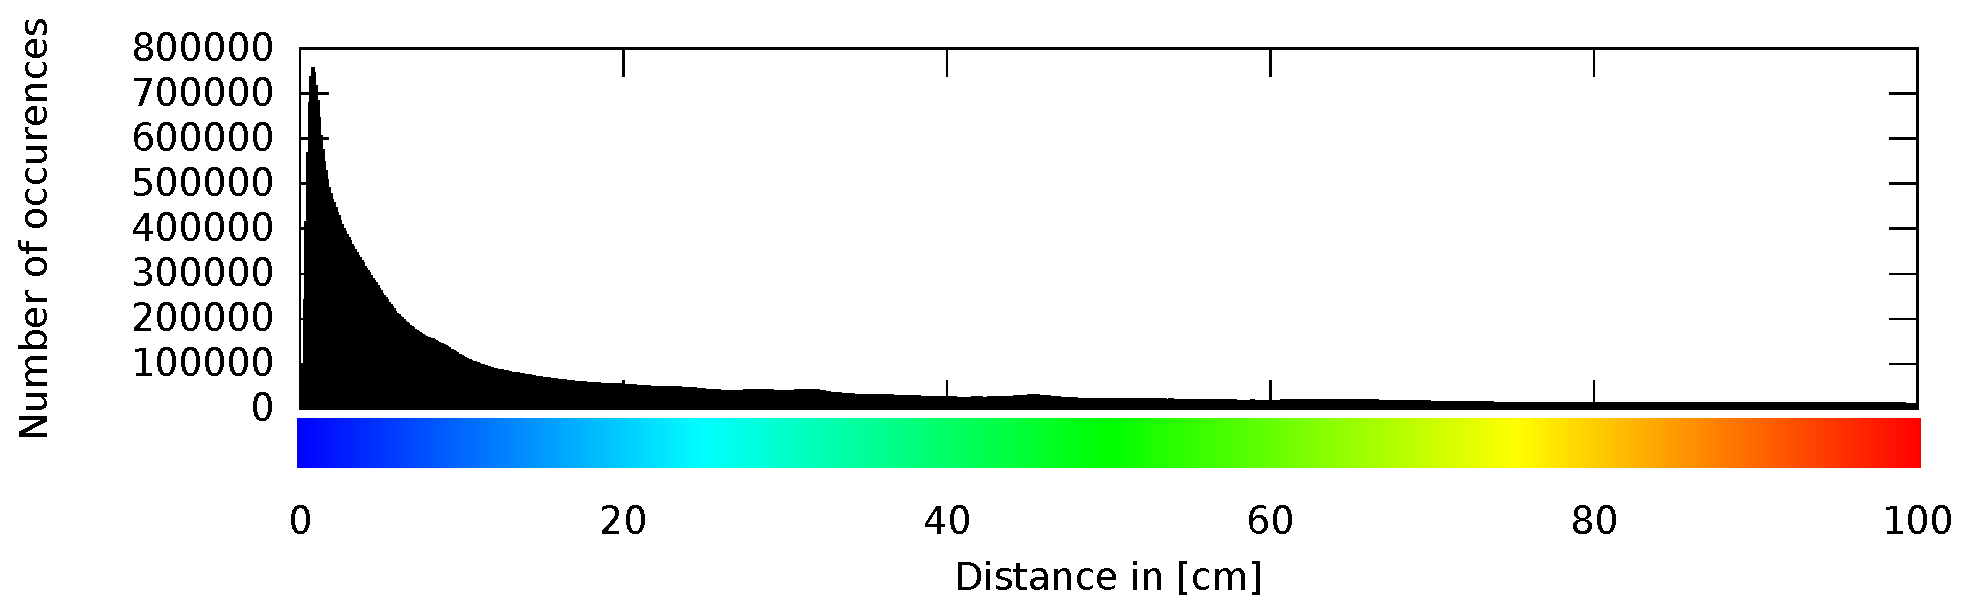
\includegraphics[width = \textwidth]{./images/histogram_fire}
	  	\end{minipage}\hfill
	  	\begin{minipage}[c]{0.25\textwidth}
	  	\end{minipage} 	

		\todo[inline]{Evaluate Plane matching on firefighter school data; histogram after etc}
		\caption{Evaluation of point distances before (left) and after (right) the plane based registration on a experimentally acquired dataset. A maximal distance of \SI{5}{m} is set, such that all points that display a higher distance value are excluded. The left column shows a heat map of distances while the right shows the corresponding histogram. The color mapping is equivalent in both. An animation of the matching process can be seen \href{todo}{here}}
		\label{fig:experimentalEvaluation}
	\end{figure}
\fi

%!TEX root = ../main.tex
\section{Conclusion}

In this paper, we propose a registration method for man made environments that exploits the structure of those environments. 
Given that in human-made environments parallel planes and right angles are abundantly available, we employ point-to-plane correspondences to improve a pre-registered 3D point cloud. 
We evaluate the procedure on a simulated dataset and on an experimentally acquired dataset with different motion profiles. 
In this evaluation, we show that the procedure improves both datasets and yields more human-made, structure-slike maps. 
In particular, the qualitative structure of the environments is reconstructed well. 
In the resulting maps, the parallel walls are clearly improved.

However, as section \ref{sec:experimentalSetup} shows, some outliers remain due to the simplistic point-to-plane correspondence model, which is to be improved in future studies.
One idea to do so is to employ a local clustering technique onto the individual scans before registering them globally. 
Points from the scan with a similar normal get clustered together if their distance is small enough.
This way, a cluster represents a local plane while at the same time storing all the points that belong to that plane.
Point-to-plane correspondences then arise from the intersection of local clusters with global planes.

Currently, not all steps in the procedure are autonomous, in particular the parameter tuning. 
In the future, one goal is to increase the autonomy of the system.
One approach is to introduce soft-locks for the optimization dimensions.
I.e., instead of locking some dimensions entirely from being used for optimization, they are weighted based on the dynamics of the system that encode which noise source is more likely.  


%!TEX root = ../main.tex
\section*{Acknowledgement}
\todo[inline]{Formulate these: ESA funding (?), elite netzwerk bayern (?)}

We thank the Cylon team (Timothy Randolph, Ignacio Dorado, Camilo Andres Reyes) for providing the dataset and documentation of the experimental setup used in this work.

\bibliography{mybibfile,andreas_publications}

\end{document}
